\chapter{DUNE Near Detector driven reweighting}
\label{sec:dune_ndrwt}

\section{Measurements of pion multiplicity}

\subsection{Gaseous argon}

\begin{figure}[h]
	\begin{minipage}[t]{.5\linewidth}
		\begin{adjustbox}{max totalsize=\linewidth, center}
			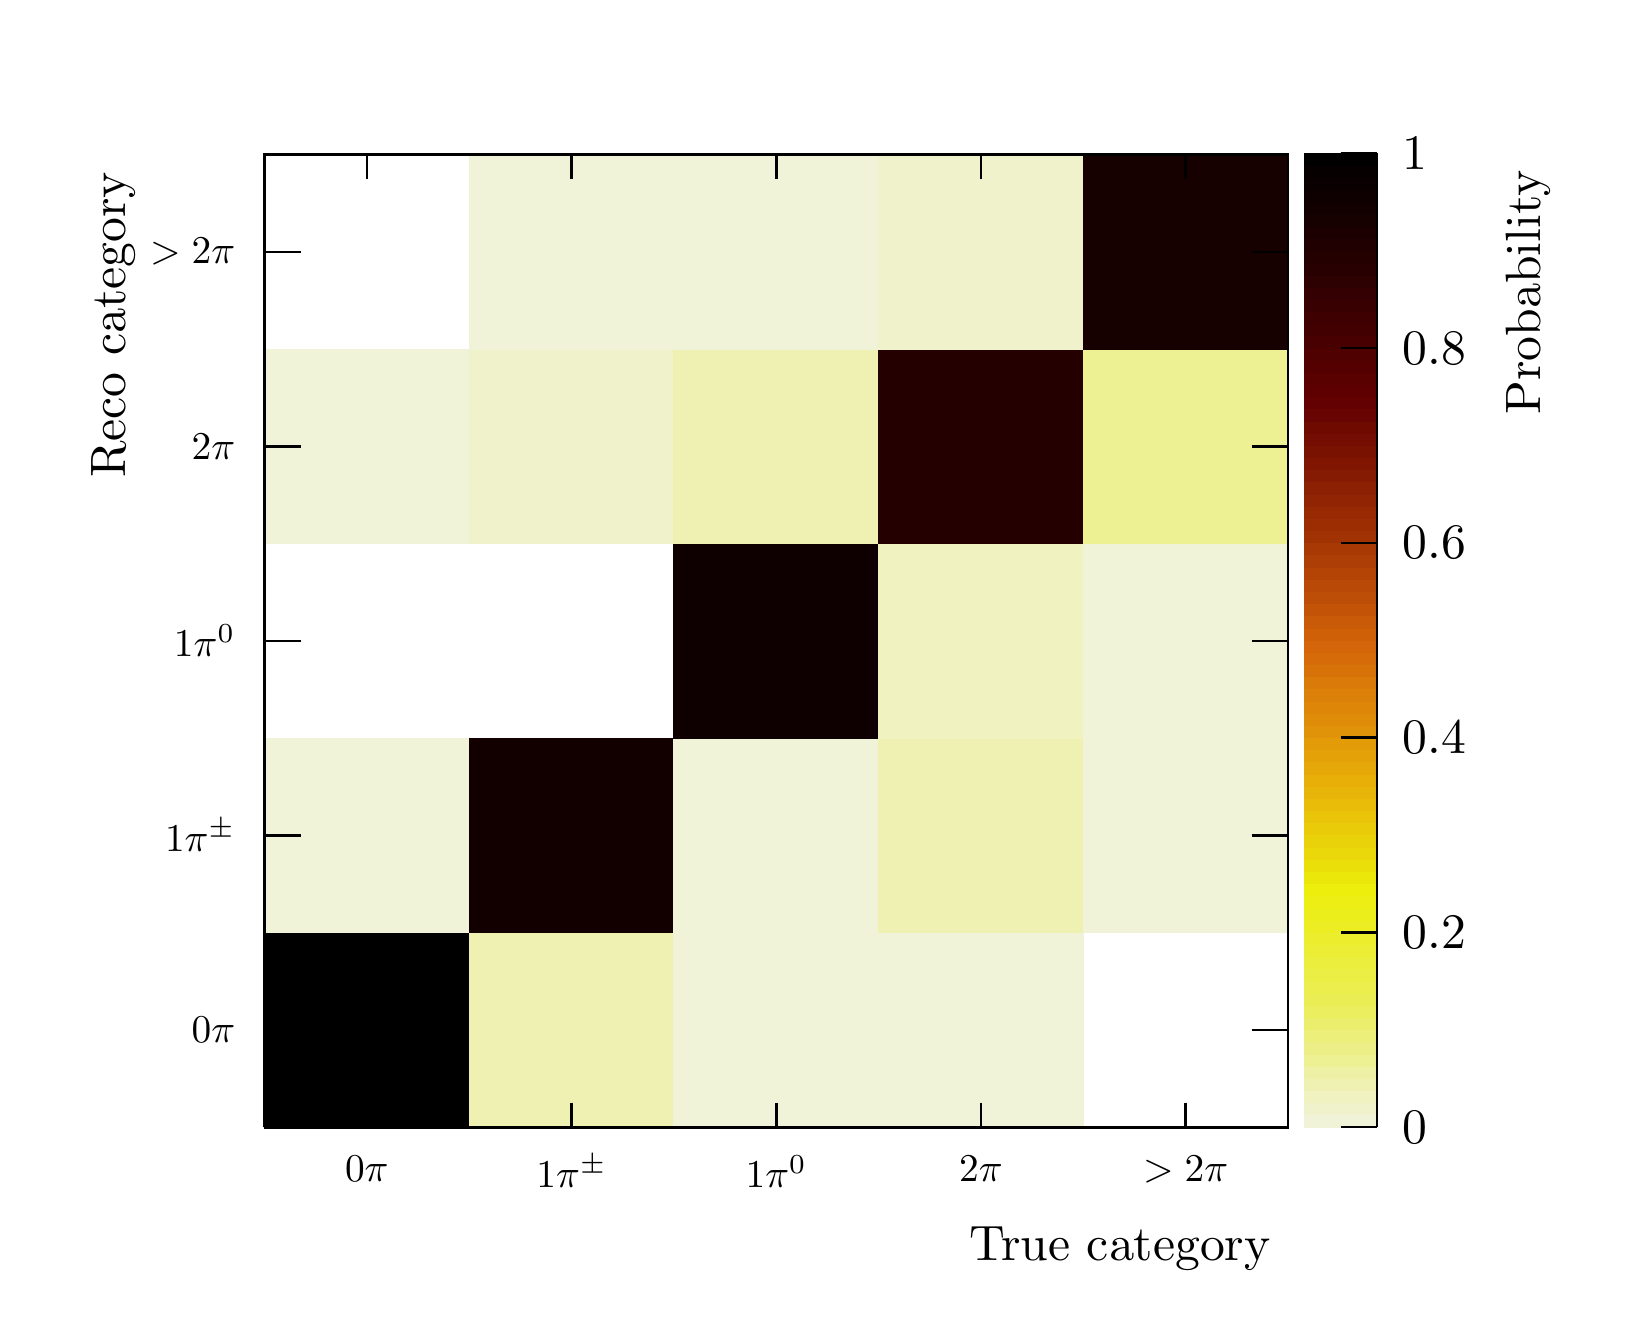
\begin{tikzpicture}
\pgfdeclareplotmark{cross} {
\pgfpathmoveto{\pgfpoint{-0.3\pgfplotmarksize}{\pgfplotmarksize}}
\pgfpathlineto{\pgfpoint{+0.3\pgfplotmarksize}{\pgfplotmarksize}}
\pgfpathlineto{\pgfpoint{+0.3\pgfplotmarksize}{0.3\pgfplotmarksize}}
\pgfpathlineto{\pgfpoint{+1\pgfplotmarksize}{0.3\pgfplotmarksize}}
\pgfpathlineto{\pgfpoint{+1\pgfplotmarksize}{-0.3\pgfplotmarksize}}
\pgfpathlineto{\pgfpoint{+0.3\pgfplotmarksize}{-0.3\pgfplotmarksize}}
\pgfpathlineto{\pgfpoint{+0.3\pgfplotmarksize}{-1.\pgfplotmarksize}}
\pgfpathlineto{\pgfpoint{-0.3\pgfplotmarksize}{-1.\pgfplotmarksize}}
\pgfpathlineto{\pgfpoint{-0.3\pgfplotmarksize}{-0.3\pgfplotmarksize}}
\pgfpathlineto{\pgfpoint{-1.\pgfplotmarksize}{-0.3\pgfplotmarksize}}
\pgfpathlineto{\pgfpoint{-1.\pgfplotmarksize}{0.3\pgfplotmarksize}}
\pgfpathlineto{\pgfpoint{-0.3\pgfplotmarksize}{0.3\pgfplotmarksize}}
\pgfpathclose
\pgfusepathqstroke
}
\pgfdeclareplotmark{cross*} {
\pgfpathmoveto{\pgfpoint{-0.3\pgfplotmarksize}{\pgfplotmarksize}}
\pgfpathlineto{\pgfpoint{+0.3\pgfplotmarksize}{\pgfplotmarksize}}
\pgfpathlineto{\pgfpoint{+0.3\pgfplotmarksize}{0.3\pgfplotmarksize}}
\pgfpathlineto{\pgfpoint{+1\pgfplotmarksize}{0.3\pgfplotmarksize}}
\pgfpathlineto{\pgfpoint{+1\pgfplotmarksize}{-0.3\pgfplotmarksize}}
\pgfpathlineto{\pgfpoint{+0.3\pgfplotmarksize}{-0.3\pgfplotmarksize}}
\pgfpathlineto{\pgfpoint{+0.3\pgfplotmarksize}{-1.\pgfplotmarksize}}
\pgfpathlineto{\pgfpoint{-0.3\pgfplotmarksize}{-1.\pgfplotmarksize}}
\pgfpathlineto{\pgfpoint{-0.3\pgfplotmarksize}{-0.3\pgfplotmarksize}}
\pgfpathlineto{\pgfpoint{-1.\pgfplotmarksize}{-0.3\pgfplotmarksize}}
\pgfpathlineto{\pgfpoint{-1.\pgfplotmarksize}{0.3\pgfplotmarksize}}
\pgfpathlineto{\pgfpoint{-0.3\pgfplotmarksize}{0.3\pgfplotmarksize}}
\pgfpathclose
\pgfusepathqfillstroke
}
\pgfdeclareplotmark{newstar} {
\pgfpathmoveto{\pgfqpoint{0pt}{\pgfplotmarksize}}
\pgfpathlineto{\pgfqpointpolar{44}{0.5\pgfplotmarksize}}
\pgfpathlineto{\pgfqpointpolar{18}{\pgfplotmarksize}}
\pgfpathlineto{\pgfqpointpolar{-20}{0.5\pgfplotmarksize}}
\pgfpathlineto{\pgfqpointpolar{-54}{\pgfplotmarksize}}
\pgfpathlineto{\pgfqpointpolar{-90}{0.5\pgfplotmarksize}}
\pgfpathlineto{\pgfqpointpolar{234}{\pgfplotmarksize}}
\pgfpathlineto{\pgfqpointpolar{198}{0.5\pgfplotmarksize}}
\pgfpathlineto{\pgfqpointpolar{162}{\pgfplotmarksize}}
\pgfpathlineto{\pgfqpointpolar{134}{0.5\pgfplotmarksize}}
\pgfpathclose
\pgfusepathqstroke
}
\pgfdeclareplotmark{newstar*} {
\pgfpathmoveto{\pgfqpoint{0pt}{\pgfplotmarksize}}
\pgfpathlineto{\pgfqpointpolar{44}{0.5\pgfplotmarksize}}
\pgfpathlineto{\pgfqpointpolar{18}{\pgfplotmarksize}}
\pgfpathlineto{\pgfqpointpolar{-20}{0.5\pgfplotmarksize}}
\pgfpathlineto{\pgfqpointpolar{-54}{\pgfplotmarksize}}
\pgfpathlineto{\pgfqpointpolar{-90}{0.5\pgfplotmarksize}}
\pgfpathlineto{\pgfqpointpolar{234}{\pgfplotmarksize}}
\pgfpathlineto{\pgfqpointpolar{198}{0.5\pgfplotmarksize}}
\pgfpathlineto{\pgfqpointpolar{162}{\pgfplotmarksize}}
\pgfpathlineto{\pgfqpointpolar{134}{0.5\pgfplotmarksize}}
\pgfpathclose
\pgfusepathqfillstroke
}
\definecolor{c}{rgb}{1,1,1};
\draw [color=c, fill=c] (0,0) rectangle (20,16.0446);
\draw [color=c, fill=c] (3,2.08579) rectangle (16,14.4401);
\definecolor{c}{rgb}{0,0,0};
\draw [c,line width=0.9] (3,2.08579) -- (3,14.4401) -- (16,14.4401) -- (16,2.08579) -- (3,2.08579);
\definecolor{c}{rgb}{1,1,1};
\draw [color=c, fill=c] (3,2.08579) rectangle (16,14.4401);
\definecolor{c}{rgb}{0,0,0};
\draw [c,line width=0.9] (3,2.08579) -- (3,14.4401) -- (16,14.4401) -- (16,2.08579) -- (3,2.08579);
\definecolor{c}{rgb}{0.00551471,0,0.000122549};
\draw [color=c, fill=c] (3,2.08579) rectangle (5.6,4.55666);
\definecolor{c}{rgb}{0.936875,0.945351,0.697027};
\draw [color=c, fill=c] (5.6,2.08579) rectangle (8.2,4.55666);
\definecolor{c}{rgb}{0.945984,0.951044,0.850727};
\draw [color=c, fill=c] (8.2,2.08579) rectangle (10.8,4.55666);
\draw [color=c, fill=c] (10.8,2.08579) rectangle (13.4,4.55666);
\draw [color=c, fill=c] (3,4.55666) rectangle (5.6,7.02752);
\definecolor{c}{rgb}{0.0716912,0,0.00159314};
\draw [color=c, fill=c] (5.6,4.55666) rectangle (8.2,7.02752);
\definecolor{c}{rgb}{0.945984,0.951044,0.850727};
\draw [color=c, fill=c] (8.2,4.55666) rectangle (10.8,7.02752);
\definecolor{c}{rgb}{0.936875,0.945351,0.697027};
\draw [color=c, fill=c] (10.8,4.55666) rectangle (13.4,7.02752);
\definecolor{c}{rgb}{0.945984,0.951044,0.850727};
\draw [color=c, fill=c] (13.4,4.55666) rectangle (16,7.02752);
\definecolor{c}{rgb}{0.0551471,0,0.00122549};
\draw [color=c, fill=c] (8.2,7.02752) rectangle (10.8,9.49838);
\definecolor{c}{rgb}{0.939911,0.947249,0.748261};
\draw [color=c, fill=c] (10.8,7.02752) rectangle (13.4,9.49838);
\definecolor{c}{rgb}{0.945984,0.951044,0.850727};
\draw [color=c, fill=c] (13.4,7.02752) rectangle (16,9.49838);
\draw [color=c, fill=c] (3,9.49838) rectangle (5.6,11.9692);
\definecolor{c}{rgb}{0.942948,0.949146,0.799494};
\draw [color=c, fill=c] (5.6,9.49838) rectangle (8.2,11.9692);
\definecolor{c}{rgb}{0.936875,0.945351,0.697027};
\draw [color=c, fill=c] (8.2,9.49838) rectangle (10.8,11.9692);
\definecolor{c}{rgb}{0.143382,0,0.00318627};
\draw [color=c, fill=c] (10.8,9.49838) rectangle (13.4,11.9692);
\definecolor{c}{rgb}{0.929791,0.940923,0.577483};
\draw [color=c, fill=c] (13.4,9.49838) rectangle (16,11.9692);
\definecolor{c}{rgb}{0.945984,0.951044,0.850727};
\draw [color=c, fill=c] (5.6,11.9692) rectangle (8.2,14.4401);
\draw [color=c, fill=c] (8.2,11.9692) rectangle (10.8,14.4401);
\definecolor{c}{rgb}{0.942948,0.949146,0.799494};
\draw [color=c, fill=c] (10.8,11.9692) rectangle (13.4,14.4401);
\definecolor{c}{rgb}{0.0882353,0,0.00196078};
\draw [color=c, fill=c] (13.4,11.9692) rectangle (16,14.4401);
\definecolor{c}{rgb}{0,0,0};
\draw [c,line width=0.9] (3,2.08579) -- (16,2.08579);
\draw [anchor=north] (4.3,1.90048) node[scale=1.42291, color=c, rotate=0]{$0\pi$};
\draw [anchor=north] (6.9,1.90048) node[scale=1.42291, color=c, rotate=0]{$1\pi^{\pm}$};
\draw [anchor=north] (9.5,1.90048) node[scale=1.42291, color=c, rotate=0]{$1\pi^{0}$};
\draw [anchor=north] (12.1,1.90048) node[scale=1.42291, color=c, rotate=0]{$2\pi$};
\draw [anchor=north] (14.7,1.90048) node[scale=1.42291, color=c, rotate=0]{$>2\pi$};
\draw [c,line width=0.9] (4.3,2.39866) -- (4.3,2.08579);
\draw [c,line width=0.9] (6.9,2.39866) -- (6.9,2.08579);
\draw [c,line width=0.9] (9.5,2.39866) -- (9.5,2.08579);
\draw [c,line width=0.9] (12.1,2.39866) -- (12.1,2.08579);
\draw [c,line width=0.9] (14.7,2.39866) -- (14.7,2.08579);
\draw [c,line width=0.9] (4.3,2.39866) -- (4.3,2.08579);
\draw [c,line width=0.9] (14.7,2.39866) -- (14.7,2.08579);
\draw [anchor= east] (16,0.545515) node[scale=1.7941, color=c, rotate=0]{ True category};
\draw [c,line width=0.9] (3,14.4401) -- (16,14.4401);
\draw [c,line width=0.9] (4.3,14.1272) -- (4.3,14.4401);
\draw [c,line width=0.9] (6.9,14.1272) -- (6.9,14.4401);
\draw [c,line width=0.9] (9.5,14.1272) -- (9.5,14.4401);
\draw [c,line width=0.9] (12.1,14.1272) -- (12.1,14.4401);
\draw [c,line width=0.9] (14.7,14.1272) -- (14.7,14.4401);
\draw [c,line width=0.9] (4.3,14.1272) -- (4.3,14.4401);
\draw [c,line width=0.9] (14.7,14.1272) -- (14.7,14.4401);
\draw [c,line width=0.9] (3,2.08579) -- (3,14.4401);
\draw [anchor= east] (2.805,3.32123) node[scale=1.42291, color=c, rotate=0]{$0\pi$};
\draw [anchor= east] (2.805,5.79209) node[scale=1.42291, color=c, rotate=0]{$1\pi^{\pm}$};
\draw [anchor= east] (2.805,8.26295) node[scale=1.42291, color=c, rotate=0]{$1\pi^{0}$};
\draw [anchor= east] (2.805,10.7338) node[scale=1.42291, color=c, rotate=0]{$2\pi$};
\draw [anchor= east] (2.805,13.2047) node[scale=1.42291, color=c, rotate=0]{$>2\pi$};
\draw [c,line width=0.9] (3.462,3.32123) -- (3,3.32123);
\draw [c,line width=0.9] (3.462,5.79209) -- (3,5.79209);
\draw [c,line width=0.9] (3.462,8.26295) -- (3,8.26295);
\draw [c,line width=0.9] (3.462,10.7338) -- (3,10.7338);
\draw [c,line width=0.9] (3.462,13.2047) -- (3,13.2047);
\draw [c,line width=0.9] (3.462,3.32123) -- (3,3.32123);
\draw [c,line width=0.9] (3.462,13.2047) -- (3,13.2047);
\draw [anchor= east] (1.08,14.4401) node[scale=1.7941, color=c, rotate=90]{ Reco category};
\draw [c,line width=0.9] (16,2.08579) -- (16,14.4401);
\draw [c,line width=0.9] (15.538,3.32123) -- (16,3.32123);
\draw [c,line width=0.9] (15.538,5.79209) -- (16,5.79209);
\draw [c,line width=0.9] (15.538,8.26295) -- (16,8.26295);
\draw [c,line width=0.9] (15.538,10.7338) -- (16,10.7338);
\draw [c,line width=0.9] (15.538,13.2047) -- (16,13.2047);
\draw [c,line width=0.9] (15.538,3.32123) -- (16,3.32123);
\draw [c,line width=0.9] (15.538,13.2047) -- (16,13.2047);
\definecolor{c}{rgb}{0.945984,0.951044,0.850727};
\draw [color=c, fill=c] (16.2117,2.08914) rectangle (17.1309,2.24373);
\definecolor{c}{rgb}{0.942948,0.949146,0.799494};
\draw [color=c, fill=c] (16.2117,2.24373) rectangle (17.1309,2.39833);
\definecolor{c}{rgb}{0.939911,0.947249,0.748261};
\draw [color=c, fill=c] (16.2117,2.39833) rectangle (17.1309,2.55292);
\definecolor{c}{rgb}{0.936875,0.945351,0.697027};
\draw [color=c, fill=c] (16.2117,2.55292) rectangle (17.1309,2.70752);
\definecolor{c}{rgb}{0.933839,0.943453,0.645794};
\draw [color=c, fill=c] (16.2117,2.70752) rectangle (17.1309,2.86212);
\definecolor{c}{rgb}{0.929791,0.940923,0.577483};
\draw [color=c, fill=c] (16.2117,2.86212) rectangle (17.1309,3.01671);
\definecolor{c}{rgb}{0.926755,0.939026,0.526249};
\draw [color=c, fill=c] (16.2117,3.01671) rectangle (17.1309,3.17131);
\definecolor{c}{rgb}{0.923719,0.937128,0.475016};
\draw [color=c, fill=c] (16.2117,3.17131) rectangle (17.1309,3.32591);
\definecolor{c}{rgb}{0.920683,0.935231,0.423782};
\draw [color=c, fill=c] (16.2117,3.32591) rectangle (17.1309,3.4805);
\definecolor{c}{rgb}{0.917647,0.933333,0.372549};
\draw [color=c, fill=c] (16.2117,3.4805) rectangle (17.1309,3.6351);
\definecolor{c}{rgb}{0.919118,0.933333,0.331373};
\draw [color=c, fill=c] (16.2117,3.6351) rectangle (17.1309,3.78969);
\definecolor{c}{rgb}{0.920221,0.933333,0.30049};
\draw [color=c, fill=c] (16.2117,3.78969) rectangle (17.1309,3.94429);
\definecolor{c}{rgb}{0.921324,0.933333,0.269608};
\draw [color=c, fill=c] (16.2117,3.94429) rectangle (17.1309,4.09889);
\definecolor{c}{rgb}{0.922426,0.933333,0.238725};
\draw [color=c, fill=c] (16.2117,4.09889) rectangle (17.1309,4.25348);
\definecolor{c}{rgb}{0.923529,0.933333,0.207843};
\draw [color=c, fill=c] (16.2117,4.25348) rectangle (17.1309,4.40808);
\definecolor{c}{rgb}{0.924632,0.933333,0.176961};
\draw [color=c, fill=c] (16.2117,4.40808) rectangle (17.1309,4.56267);
\definecolor{c}{rgb}{0.926103,0.933333,0.135784};
\draw [color=c, fill=c] (16.2117,4.56267) rectangle (17.1309,4.71727);
\definecolor{c}{rgb}{0.927206,0.933333,0.104902};
\draw [color=c, fill=c] (16.2117,4.71727) rectangle (17.1309,4.87187);
\definecolor{c}{rgb}{0.928309,0.933333,0.0740196};
\draw [color=c, fill=c] (16.2117,4.87187) rectangle (17.1309,5.02646);
\definecolor{c}{rgb}{0.929412,0.933333,0.0431373};
\draw [color=c, fill=c] (16.2117,5.02646) rectangle (17.1309,5.18106);
\definecolor{c}{rgb}{0.926838,0.907598,0.0420343};
\draw [color=c, fill=c] (16.2117,5.18106) rectangle (17.1309,5.33565);
\definecolor{c}{rgb}{0.923407,0.873284,0.0405637};
\draw [color=c, fill=c] (16.2117,5.33565) rectangle (17.1309,5.49025);
\definecolor{c}{rgb}{0.920833,0.847549,0.0394608};
\draw [color=c, fill=c] (16.2117,5.49025) rectangle (17.1309,5.64485);
\definecolor{c}{rgb}{0.91826,0.821814,0.0383578};
\draw [color=c, fill=c] (16.2117,5.64485) rectangle (17.1309,5.79944);
\definecolor{c}{rgb}{0.915686,0.796078,0.0372549};
\draw [color=c, fill=c] (16.2117,5.79944) rectangle (17.1309,5.95404);
\definecolor{c}{rgb}{0.913113,0.770343,0.036152};
\draw [color=c, fill=c] (16.2117,5.95404) rectangle (17.1309,6.10864);
\definecolor{c}{rgb}{0.909681,0.736029,0.0346814};
\draw [color=c, fill=c] (16.2117,6.10864) rectangle (17.1309,6.26323);
\definecolor{c}{rgb}{0.907108,0.710294,0.0335784};
\draw [color=c, fill=c] (16.2117,6.26323) rectangle (17.1309,6.41783);
\definecolor{c}{rgb}{0.904534,0.684559,0.0324755};
\draw [color=c, fill=c] (16.2117,6.41783) rectangle (17.1309,6.57242);
\definecolor{c}{rgb}{0.901961,0.658824,0.0313726};
\draw [color=c, fill=c] (16.2117,6.57242) rectangle (17.1309,6.72702);
\definecolor{c}{rgb}{0.895343,0.634191,0.0317402};
\draw [color=c, fill=c] (16.2117,6.72702) rectangle (17.1309,6.88162);
\definecolor{c}{rgb}{0.888726,0.609559,0.0321078};
\draw [color=c, fill=c] (16.2117,6.88162) rectangle (17.1309,7.03621);
\definecolor{c}{rgb}{0.879902,0.576716,0.032598};
\draw [color=c, fill=c] (16.2117,7.03621) rectangle (17.1309,7.19081);
\definecolor{c}{rgb}{0.873284,0.552083,0.0329657};
\draw [color=c, fill=c] (16.2117,7.19081) rectangle (17.1309,7.3454);
\definecolor{c}{rgb}{0.866667,0.527451,0.0333333};
\draw [color=c, fill=c] (16.2117,7.3454) rectangle (17.1309,7.5);
\definecolor{c}{rgb}{0.860049,0.502819,0.033701};
\draw [color=c, fill=c] (16.2117,7.5) rectangle (17.1309,7.6546);
\definecolor{c}{rgb}{0.853431,0.478186,0.0340686};
\draw [color=c, fill=c] (16.2117,7.6546) rectangle (17.1309,7.80919);
\definecolor{c}{rgb}{0.844608,0.445343,0.0345588};
\draw [color=c, fill=c] (16.2117,7.80919) rectangle (17.1309,7.96379);
\definecolor{c}{rgb}{0.83799,0.420711,0.0349265};
\draw [color=c, fill=c] (16.2117,7.96379) rectangle (17.1309,8.11838);
\definecolor{c}{rgb}{0.831373,0.396078,0.0352941};
\draw [color=c, fill=c] (16.2117,8.11838) rectangle (17.1309,8.27298);
\definecolor{c}{rgb}{0.810784,0.37549,0.0330882};
\draw [color=c, fill=c] (16.2117,8.27298) rectangle (17.1309,8.42758);
\definecolor{c}{rgb}{0.790196,0.354902,0.0308824};
\draw [color=c, fill=c] (16.2117,8.42758) rectangle (17.1309,8.58217);
\definecolor{c}{rgb}{0.762745,0.327451,0.0279412};
\draw [color=c, fill=c] (16.2117,8.58217) rectangle (17.1309,8.73677);
\definecolor{c}{rgb}{0.742157,0.306863,0.0257353};
\draw [color=c, fill=c] (16.2117,8.73677) rectangle (17.1309,8.89137);
\definecolor{c}{rgb}{0.721569,0.286275,0.0235294};
\draw [color=c, fill=c] (16.2117,8.89137) rectangle (17.1309,9.04596);
\definecolor{c}{rgb}{0.70098,0.265686,0.0213235};
\draw [color=c, fill=c] (16.2117,9.04596) rectangle (17.1309,9.20056);
\definecolor{c}{rgb}{0.680392,0.245098,0.0191176};
\draw [color=c, fill=c] (16.2117,9.20056) rectangle (17.1309,9.35515);
\definecolor{c}{rgb}{0.659804,0.22451,0.0169118};
\draw [color=c, fill=c] (16.2117,9.35515) rectangle (17.1309,9.50975);
\definecolor{c}{rgb}{0.632353,0.197059,0.0139706};
\draw [color=c, fill=c] (16.2117,9.50975) rectangle (17.1309,9.66435);
\definecolor{c}{rgb}{0.611765,0.176471,0.0117647};
\draw [color=c, fill=c] (16.2117,9.66435) rectangle (17.1309,9.81894);
\definecolor{c}{rgb}{0.590809,0.159926,0.0110294};
\draw [color=c, fill=c] (16.2117,9.81894) rectangle (17.1309,9.97354);
\definecolor{c}{rgb}{0.569853,0.143382,0.0102941};
\draw [color=c, fill=c] (16.2117,9.97354) rectangle (17.1309,10.1281);
\definecolor{c}{rgb}{0.548897,0.126838,0.00955882};
\draw [color=c, fill=c] (16.2117,10.1281) rectangle (17.1309,10.2827);
\definecolor{c}{rgb}{0.520956,0.104779,0.00857843};
\draw [color=c, fill=c] (16.2117,10.2827) rectangle (17.1309,10.4373);
\definecolor{c}{rgb}{0.5,0.0882353,0.00784314};
\draw [color=c, fill=c] (16.2117,10.4373) rectangle (17.1309,10.5919);
\definecolor{c}{rgb}{0.479044,0.0716912,0.00710784};
\draw [color=c, fill=c] (16.2117,10.5919) rectangle (17.1309,10.7465);
\definecolor{c}{rgb}{0.458088,0.0551471,0.00637255};
\draw [color=c, fill=c] (16.2117,10.7465) rectangle (17.1309,10.9011);
\definecolor{c}{rgb}{0.437132,0.0386029,0.00563726};
\draw [color=c, fill=c] (16.2117,10.9011) rectangle (17.1309,11.0557);
\definecolor{c}{rgb}{0.409191,0.0165441,0.00465686};
\draw [color=c, fill=c] (16.2117,11.0557) rectangle (17.1309,11.2103);
\definecolor{c}{rgb}{0.388235,0,0.00392157};
\draw [color=c, fill=c] (16.2117,11.2103) rectangle (17.1309,11.3649);
\definecolor{c}{rgb}{0.368382,0,0.00392157};
\draw [color=c, fill=c] (16.2117,11.3649) rectangle (17.1309,11.5195);
\definecolor{c}{rgb}{0.348529,0,0.00392157};
\draw [color=c, fill=c] (16.2117,11.5195) rectangle (17.1309,11.6741);
\definecolor{c}{rgb}{0.328676,0,0.00392157};
\draw [color=c, fill=c] (16.2117,11.6741) rectangle (17.1309,11.8287);
\definecolor{c}{rgb}{0.308824,0,0.00392157};
\draw [color=c, fill=c] (16.2117,11.8287) rectangle (17.1309,11.9833);
\definecolor{c}{rgb}{0.282353,0,0.00392157};
\draw [color=c, fill=c] (16.2117,11.9833) rectangle (17.1309,12.1379);
\definecolor{c}{rgb}{0.2625,0,0.00392157};
\draw [color=c, fill=c] (16.2117,12.1379) rectangle (17.1309,12.2925);
\definecolor{c}{rgb}{0.242647,0,0.00392157};
\draw [color=c, fill=c] (16.2117,12.2925) rectangle (17.1309,12.4471);
\definecolor{c}{rgb}{0.222794,0,0.00392157};
\draw [color=c, fill=c] (16.2117,12.4471) rectangle (17.1309,12.6017);
\definecolor{c}{rgb}{0.202941,0,0.00392157};
\draw [color=c, fill=c] (16.2117,12.6017) rectangle (17.1309,12.7563);
\definecolor{c}{rgb}{0.176471,0,0.00392157};
\draw [color=c, fill=c] (16.2117,12.7563) rectangle (17.1309,12.9109);
\definecolor{c}{rgb}{0.159926,0,0.00355392};
\draw [color=c, fill=c] (16.2117,12.9109) rectangle (17.1309,13.0655);
\definecolor{c}{rgb}{0.143382,0,0.00318627};
\draw [color=c, fill=c] (16.2117,13.0655) rectangle (17.1309,13.2201);
\definecolor{c}{rgb}{0.126838,0,0.00281863};
\draw [color=c, fill=c] (16.2117,13.2201) rectangle (17.1309,13.3747);
\definecolor{c}{rgb}{0.110294,0,0.00245098};
\draw [color=c, fill=c] (16.2117,13.3747) rectangle (17.1309,13.5292);
\definecolor{c}{rgb}{0.0882353,0,0.00196078};
\draw [color=c, fill=c] (16.2117,13.5292) rectangle (17.1309,13.6838);
\definecolor{c}{rgb}{0.0716912,0,0.00159314};
\draw [color=c, fill=c] (16.2117,13.6838) rectangle (17.1309,13.8384);
\definecolor{c}{rgb}{0.0551471,0,0.00122549};
\draw [color=c, fill=c] (16.2117,13.8384) rectangle (17.1309,13.993);
\definecolor{c}{rgb}{0.0386029,0,0.000857843};
\draw [color=c, fill=c] (16.2117,13.993) rectangle (17.1309,14.1476);
\definecolor{c}{rgb}{0.0220588,0,0.000490196};
\draw [color=c, fill=c] (16.2117,14.1476) rectangle (17.1309,14.3022);
\definecolor{c}{rgb}{0.00551471,0,0.000122549};
\draw [color=c, fill=c] (16.2117,14.3022) rectangle (17.1309,14.4568);
\definecolor{c}{rgb}{0,0,0};
\draw [c,line width=0.9] (17.1309,2.08914) -- (17.1309,14.4568);
\draw [c,line width=0.9] (16.6684,2.08914) -- (17.1309,2.08914);
\draw [c,line width=0.9] (16.6684,4.56267) -- (17.1309,4.56267);
\draw [c,line width=0.9] (16.6684,7.03621) -- (17.1309,7.03621);
\draw [c,line width=0.9] (16.6684,9.50975) -- (17.1309,9.50975);
\draw [c,line width=0.9] (16.6684,11.9833) -- (17.1309,11.9833);
\draw [c,line width=0.9] (16.6684,14.4568) -- (17.1309,14.4568);
\draw [c,line width=0.9] (16.6684,14.4568) -- (17.1309,14.4568);
\draw [anchor= west] (17.2309,2.08914) node[scale=1.7941, color=c, rotate=0]{0};
\draw [anchor= west] (17.2309,4.56267) node[scale=1.7941, color=c, rotate=0]{0.2};
\draw [anchor= west] (17.2309,7.03621) node[scale=1.7941, color=c, rotate=0]{0.4};
\draw [anchor= west] (17.2309,9.50975) node[scale=1.7941, color=c, rotate=0]{0.6};
\draw [anchor= west] (17.2309,11.9833) node[scale=1.7941, color=c, rotate=0]{0.8};
\draw [anchor= west] (17.2309,14.4568) node[scale=1.7941, color=c, rotate=0]{1};
\draw [anchor= east] (19.0509,14.4568) node[scale=1.7941, color=c, rotate=90]{ Probability};
\definecolor{c}{rgb}{1,1,1};
\draw [color=c, fill=c] (2,15.0819) rectangle (18,15.9643);
\definecolor{c}{rgb}{0,0,0};
%\draw (10,15.5231) node[scale=1.67037, color=c, rotate=0]{Final state confusion matrix in HPgTPC};
\end{tikzpicture}

		\end{adjustbox}
	\end{minipage}
	\hfill
	\begin{minipage}[t]{.5\linewidth}
		\begin{adjustbox}{max totalsize=\linewidth, center}
			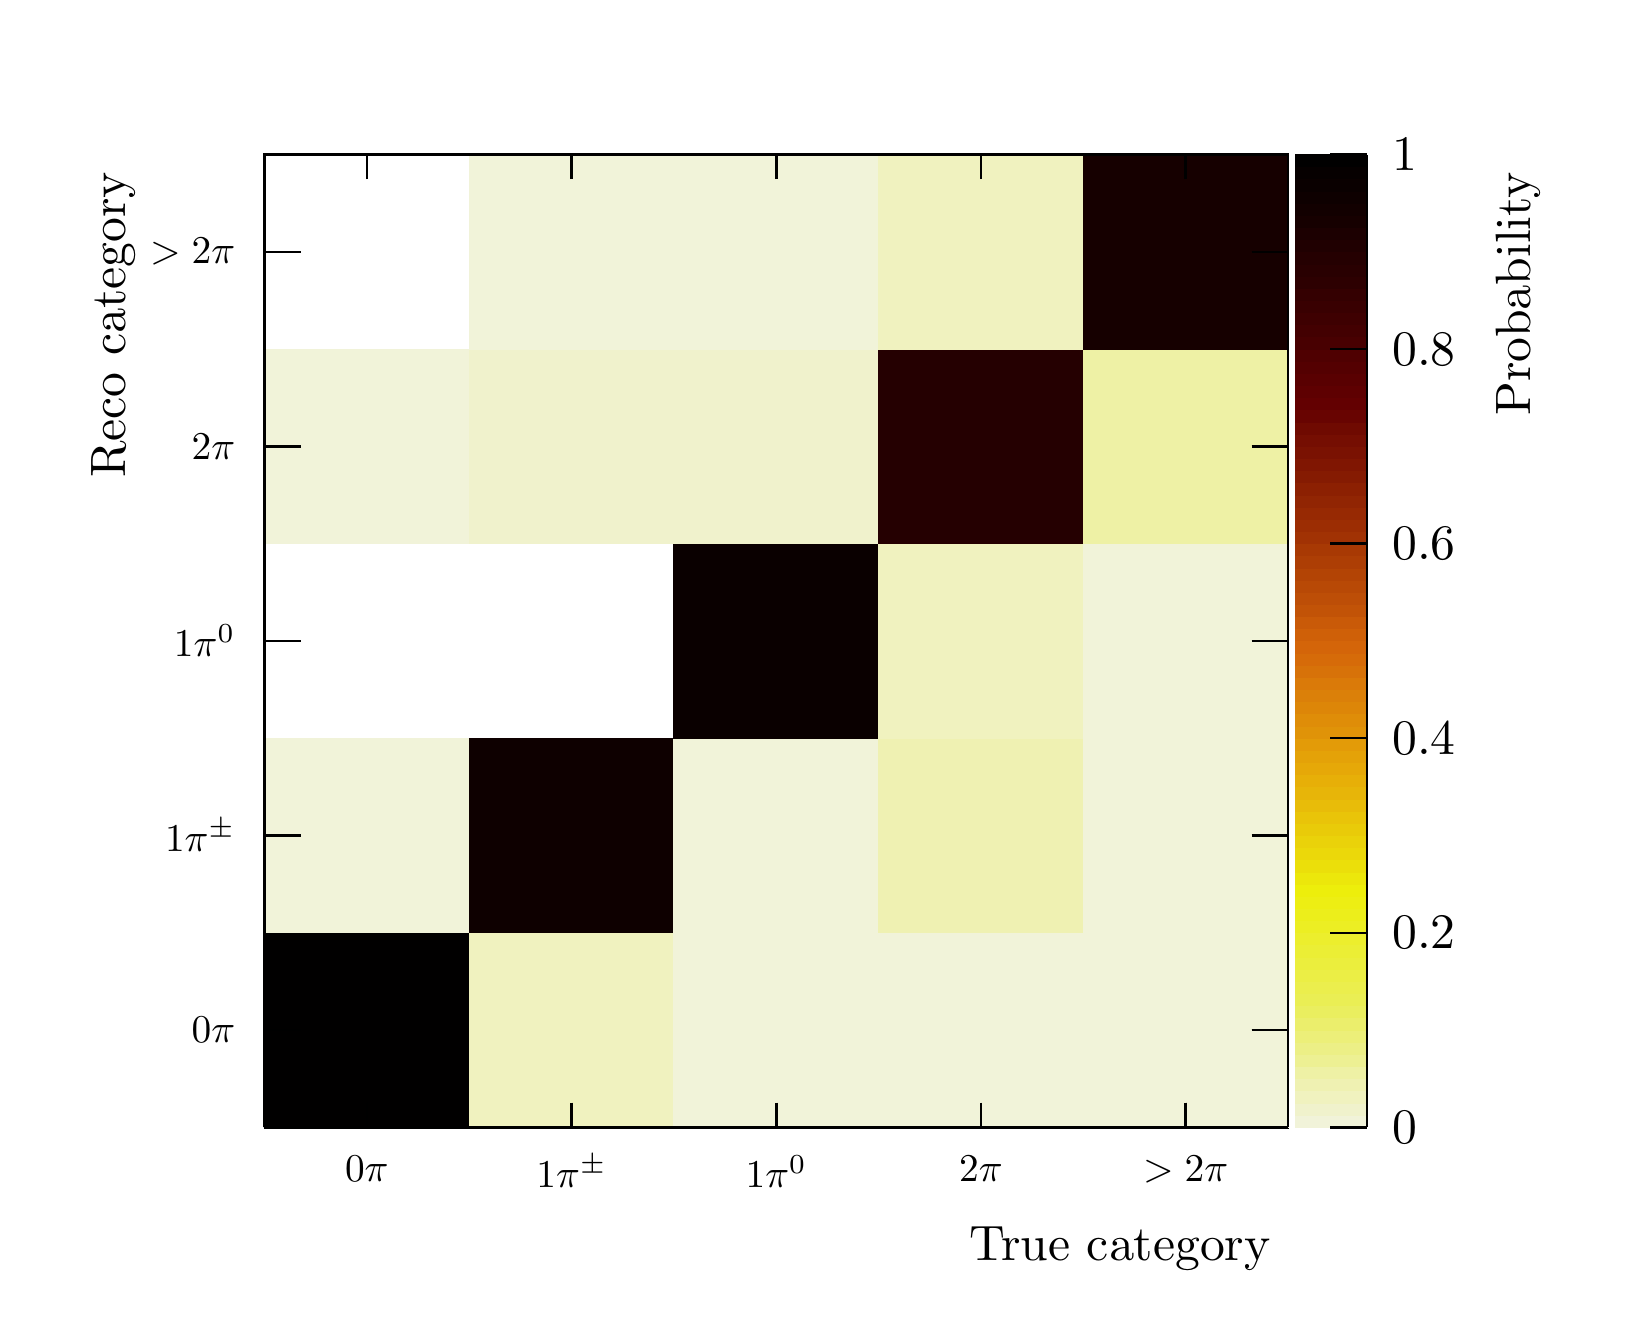
\begin{tikzpicture}
\pgfdeclareplotmark{cross} {
\pgfpathmoveto{\pgfpoint{-0.3\pgfplotmarksize}{\pgfplotmarksize}}
\pgfpathlineto{\pgfpoint{+0.3\pgfplotmarksize}{\pgfplotmarksize}}
\pgfpathlineto{\pgfpoint{+0.3\pgfplotmarksize}{0.3\pgfplotmarksize}}
\pgfpathlineto{\pgfpoint{+1\pgfplotmarksize}{0.3\pgfplotmarksize}}
\pgfpathlineto{\pgfpoint{+1\pgfplotmarksize}{-0.3\pgfplotmarksize}}
\pgfpathlineto{\pgfpoint{+0.3\pgfplotmarksize}{-0.3\pgfplotmarksize}}
\pgfpathlineto{\pgfpoint{+0.3\pgfplotmarksize}{-1.\pgfplotmarksize}}
\pgfpathlineto{\pgfpoint{-0.3\pgfplotmarksize}{-1.\pgfplotmarksize}}
\pgfpathlineto{\pgfpoint{-0.3\pgfplotmarksize}{-0.3\pgfplotmarksize}}
\pgfpathlineto{\pgfpoint{-1.\pgfplotmarksize}{-0.3\pgfplotmarksize}}
\pgfpathlineto{\pgfpoint{-1.\pgfplotmarksize}{0.3\pgfplotmarksize}}
\pgfpathlineto{\pgfpoint{-0.3\pgfplotmarksize}{0.3\pgfplotmarksize}}
\pgfpathclose
\pgfusepathqstroke
}
\pgfdeclareplotmark{cross*} {
\pgfpathmoveto{\pgfpoint{-0.3\pgfplotmarksize}{\pgfplotmarksize}}
\pgfpathlineto{\pgfpoint{+0.3\pgfplotmarksize}{\pgfplotmarksize}}
\pgfpathlineto{\pgfpoint{+0.3\pgfplotmarksize}{0.3\pgfplotmarksize}}
\pgfpathlineto{\pgfpoint{+1\pgfplotmarksize}{0.3\pgfplotmarksize}}
\pgfpathlineto{\pgfpoint{+1\pgfplotmarksize}{-0.3\pgfplotmarksize}}
\pgfpathlineto{\pgfpoint{+0.3\pgfplotmarksize}{-0.3\pgfplotmarksize}}
\pgfpathlineto{\pgfpoint{+0.3\pgfplotmarksize}{-1.\pgfplotmarksize}}
\pgfpathlineto{\pgfpoint{-0.3\pgfplotmarksize}{-1.\pgfplotmarksize}}
\pgfpathlineto{\pgfpoint{-0.3\pgfplotmarksize}{-0.3\pgfplotmarksize}}
\pgfpathlineto{\pgfpoint{-1.\pgfplotmarksize}{-0.3\pgfplotmarksize}}
\pgfpathlineto{\pgfpoint{-1.\pgfplotmarksize}{0.3\pgfplotmarksize}}
\pgfpathlineto{\pgfpoint{-0.3\pgfplotmarksize}{0.3\pgfplotmarksize}}
\pgfpathclose
\pgfusepathqfillstroke
}
\pgfdeclareplotmark{newstar} {
\pgfpathmoveto{\pgfqpoint{0pt}{\pgfplotmarksize}}
\pgfpathlineto{\pgfqpointpolar{44}{0.5\pgfplotmarksize}}
\pgfpathlineto{\pgfqpointpolar{18}{\pgfplotmarksize}}
\pgfpathlineto{\pgfqpointpolar{-20}{0.5\pgfplotmarksize}}
\pgfpathlineto{\pgfqpointpolar{-54}{\pgfplotmarksize}}
\pgfpathlineto{\pgfqpointpolar{-90}{0.5\pgfplotmarksize}}
\pgfpathlineto{\pgfqpointpolar{234}{\pgfplotmarksize}}
\pgfpathlineto{\pgfqpointpolar{198}{0.5\pgfplotmarksize}}
\pgfpathlineto{\pgfqpointpolar{162}{\pgfplotmarksize}}
\pgfpathlineto{\pgfqpointpolar{134}{0.5\pgfplotmarksize}}
\pgfpathclose
\pgfusepathqstroke
}
\pgfdeclareplotmark{newstar*} {
\pgfpathmoveto{\pgfqpoint{0pt}{\pgfplotmarksize}}
\pgfpathlineto{\pgfqpointpolar{44}{0.5\pgfplotmarksize}}
\pgfpathlineto{\pgfqpointpolar{18}{\pgfplotmarksize}}
\pgfpathlineto{\pgfqpointpolar{-20}{0.5\pgfplotmarksize}}
\pgfpathlineto{\pgfqpointpolar{-54}{\pgfplotmarksize}}
\pgfpathlineto{\pgfqpointpolar{-90}{0.5\pgfplotmarksize}}
\pgfpathlineto{\pgfqpointpolar{234}{\pgfplotmarksize}}
\pgfpathlineto{\pgfqpointpolar{198}{0.5\pgfplotmarksize}}
\pgfpathlineto{\pgfqpointpolar{162}{\pgfplotmarksize}}
\pgfpathlineto{\pgfqpointpolar{134}{0.5\pgfplotmarksize}}
\pgfpathclose
\pgfusepathqfillstroke
}
\definecolor{c}{rgb}{1,1,1};
\draw [color=c, fill=c] (0,0) rectangle (20,16.0446);
\draw [color=c, fill=c] (3,2.08579) rectangle (16,14.4401);
\definecolor{c}{rgb}{0,0,0};
\draw [c,line width=0.9] (3,2.08579) -- (3,14.4401) -- (16,14.4401) -- (16,2.08579) -- (3,2.08579);
\definecolor{c}{rgb}{1,1,1};
\draw [color=c, fill=c] (3,2.08579) rectangle (16,14.4401);
\definecolor{c}{rgb}{0,0,0};
\draw [c,line width=0.9] (3,2.08579) -- (3,14.4401) -- (16,14.4401) -- (16,2.08579) -- (3,2.08579);
\definecolor{c}{rgb}{0.00551471,0,0.000122549};
\draw [color=c, fill=c] (3,2.08579) rectangle (5.6,4.55666);
\definecolor{c}{rgb}{0.939911,0.947249,0.748261};
\draw [color=c, fill=c] (5.6,2.08579) rectangle (8.2,4.55666);
\definecolor{c}{rgb}{0.945984,0.951044,0.850727};
\draw [color=c, fill=c] (8.2,2.08579) rectangle (10.8,4.55666);
\draw [color=c, fill=c] (10.8,2.08579) rectangle (13.4,4.55666);
\draw [color=c, fill=c] (13.4,2.08579) rectangle (16,4.55666);
\draw [color=c, fill=c] (3,4.55666) rectangle (5.6,7.02752);
\definecolor{c}{rgb}{0.0551471,0,0.00122549};
\draw [color=c, fill=c] (5.6,4.55666) rectangle (8.2,7.02752);
\definecolor{c}{rgb}{0.945984,0.951044,0.850727};
\draw [color=c, fill=c] (8.2,4.55666) rectangle (10.8,7.02752);
\definecolor{c}{rgb}{0.936875,0.945351,0.697027};
\draw [color=c, fill=c] (10.8,4.55666) rectangle (13.4,7.02752);
\definecolor{c}{rgb}{0.945984,0.951044,0.850727};
\draw [color=c, fill=c] (13.4,4.55666) rectangle (16,7.02752);
\definecolor{c}{rgb}{0.0386029,0,0.000857843};
\draw [color=c, fill=c] (8.2,7.02752) rectangle (10.8,9.49838);
\definecolor{c}{rgb}{0.939911,0.947249,0.748261};
\draw [color=c, fill=c] (10.8,7.02752) rectangle (13.4,9.49838);
\definecolor{c}{rgb}{0.945984,0.951044,0.850727};
\draw [color=c, fill=c] (13.4,7.02752) rectangle (16,9.49838);
\draw [color=c, fill=c] (3,9.49838) rectangle (5.6,11.9692);
\definecolor{c}{rgb}{0.942948,0.949146,0.799494};
\draw [color=c, fill=c] (5.6,9.49838) rectangle (8.2,11.9692);
\draw [color=c, fill=c] (8.2,9.49838) rectangle (10.8,11.9692);
\definecolor{c}{rgb}{0.143382,0,0.00318627};
\draw [color=c, fill=c] (10.8,9.49838) rectangle (13.4,11.9692);
\definecolor{c}{rgb}{0.933839,0.943453,0.645794};
\draw [color=c, fill=c] (13.4,9.49838) rectangle (16,11.9692);
\definecolor{c}{rgb}{0.945984,0.951044,0.850727};
\draw [color=c, fill=c] (5.6,11.9692) rectangle (8.2,14.4401);
\draw [color=c, fill=c] (8.2,11.9692) rectangle (10.8,14.4401);
\definecolor{c}{rgb}{0.939911,0.947249,0.748261};
\draw [color=c, fill=c] (10.8,11.9692) rectangle (13.4,14.4401);
\definecolor{c}{rgb}{0.0882353,0,0.00196078};
\draw [color=c, fill=c] (13.4,11.9692) rectangle (16,14.4401);
\definecolor{c}{rgb}{0,0,0};
\draw [c,line width=0.9] (3,2.08579) -- (16,2.08579);
\draw [anchor=north] (4.3,1.90048) node[scale=1.42291, color=c, rotate=0]{$0\pi$};
\draw [anchor=north] (6.9,1.90048) node[scale=1.42291, color=c, rotate=0]{$1\pi^{\pm}$};
\draw [anchor=north] (9.5,1.90048) node[scale=1.42291, color=c, rotate=0]{$1\pi^{0}$};
\draw [anchor=north] (12.1,1.90048) node[scale=1.42291, color=c, rotate=0]{$2\pi$};
\draw [anchor=north] (14.7,1.90048) node[scale=1.42291, color=c, rotate=0]{$>2\pi$};
\draw [c,line width=0.9] (4.3,2.39866) -- (4.3,2.08579);
\draw [c,line width=0.9] (6.9,2.39866) -- (6.9,2.08579);
\draw [c,line width=0.9] (9.5,2.39866) -- (9.5,2.08579);
\draw [c,line width=0.9] (12.1,2.39866) -- (12.1,2.08579);
\draw [c,line width=0.9] (14.7,2.39866) -- (14.7,2.08579);
\draw [c,line width=0.9] (4.3,2.39866) -- (4.3,2.08579);
\draw [c,line width=0.9] (14.7,2.39866) -- (14.7,2.08579);
\draw [anchor= east] (16,0.545515) node[scale=1.7941, color=c, rotate=0]{ True category};
\draw [c,line width=0.9] (3,14.4401) -- (16,14.4401);
\draw [c,line width=0.9] (4.3,14.1272) -- (4.3,14.4401);
\draw [c,line width=0.9] (6.9,14.1272) -- (6.9,14.4401);
\draw [c,line width=0.9] (9.5,14.1272) -- (9.5,14.4401);
\draw [c,line width=0.9] (12.1,14.1272) -- (12.1,14.4401);
\draw [c,line width=0.9] (14.7,14.1272) -- (14.7,14.4401);
\draw [c,line width=0.9] (4.3,14.1272) -- (4.3,14.4401);
\draw [c,line width=0.9] (14.7,14.1272) -- (14.7,14.4401);
\draw [c,line width=0.9] (3,2.08579) -- (3,14.4401);
\draw [anchor= east] (2.805,3.32123) node[scale=1.42291, color=c, rotate=0]{$0\pi$};
\draw [anchor= east] (2.805,5.79209) node[scale=1.42291, color=c, rotate=0]{$1\pi^{\pm}$};
\draw [anchor= east] (2.805,8.26295) node[scale=1.42291, color=c, rotate=0]{$1\pi^{0}$};
\draw [anchor= east] (2.805,10.7338) node[scale=1.42291, color=c, rotate=0]{$2\pi$};
\draw [anchor= east] (2.805,13.2047) node[scale=1.42291, color=c, rotate=0]{$>2\pi$};
\draw [c,line width=0.9] (3.462,3.32123) -- (3,3.32123);
\draw [c,line width=0.9] (3.462,5.79209) -- (3,5.79209);
\draw [c,line width=0.9] (3.462,8.26295) -- (3,8.26295);
\draw [c,line width=0.9] (3.462,10.7338) -- (3,10.7338);
\draw [c,line width=0.9] (3.462,13.2047) -- (3,13.2047);
\draw [c,line width=0.9] (3.462,3.32123) -- (3,3.32123);
\draw [c,line width=0.9] (3.462,13.2047) -- (3,13.2047);
\draw [anchor= east] (1.08,14.4401) node[scale=1.7941, color=c, rotate=90]{ Reco category};
\draw [c,line width=0.9] (16,2.08579) -- (16,14.4401);
\draw [c,line width=0.9] (15.538,3.32123) -- (16,3.32123);
\draw [c,line width=0.9] (15.538,5.79209) -- (16,5.79209);
\draw [c,line width=0.9] (15.538,8.26295) -- (16,8.26295);
\draw [c,line width=0.9] (15.538,10.7338) -- (16,10.7338);
\draw [c,line width=0.9] (15.538,13.2047) -- (16,13.2047);
\draw [c,line width=0.9] (15.538,3.32123) -- (16,3.32123);
\draw [c,line width=0.9] (15.538,13.2047) -- (16,13.2047);
\definecolor{c}{rgb}{0.945984,0.951044,0.850727};
\draw [color=c, fill=c] (16.1,2.08579) rectangle (17,2.24022);
\definecolor{c}{rgb}{0.942948,0.949146,0.799494};
\draw [color=c, fill=c] (16.1,2.24022) rectangle (17,2.39465);
\definecolor{c}{rgb}{0.939911,0.947249,0.748261};
\draw [color=c, fill=c] (16.1,2.39465) rectangle (17,2.54908);
\definecolor{c}{rgb}{0.936875,0.945351,0.697027};
\draw [color=c, fill=c] (16.1,2.54908) rectangle (17,2.70351);
\definecolor{c}{rgb}{0.933839,0.943453,0.645794};
\draw [color=c, fill=c] (16.1,2.70351) rectangle (17,2.85794);
\definecolor{c}{rgb}{0.929791,0.940923,0.577483};
\draw [color=c, fill=c] (16.1,2.85794) rectangle (17,3.01237);
\definecolor{c}{rgb}{0.926755,0.939026,0.526249};
\draw [color=c, fill=c] (16.1,3.01237) rectangle (17,3.1668);
\definecolor{c}{rgb}{0.923719,0.937128,0.475016};
\draw [color=c, fill=c] (16.1,3.1668) rectangle (17,3.32123);
\definecolor{c}{rgb}{0.920683,0.935231,0.423782};
\draw [color=c, fill=c] (16.1,3.32123) rectangle (17,3.47565);
\definecolor{c}{rgb}{0.917647,0.933333,0.372549};
\draw [color=c, fill=c] (16.1,3.47565) rectangle (17,3.63008);
\definecolor{c}{rgb}{0.919118,0.933333,0.331373};
\draw [color=c, fill=c] (16.1,3.63008) rectangle (17,3.78451);
\definecolor{c}{rgb}{0.920221,0.933333,0.30049};
\draw [color=c, fill=c] (16.1,3.78451) rectangle (17,3.93894);
\definecolor{c}{rgb}{0.921324,0.933333,0.269608};
\draw [color=c, fill=c] (16.1,3.93894) rectangle (17,4.09337);
\definecolor{c}{rgb}{0.922426,0.933333,0.238725};
\draw [color=c, fill=c] (16.1,4.09337) rectangle (17,4.2478);
\definecolor{c}{rgb}{0.923529,0.933333,0.207843};
\draw [color=c, fill=c] (16.1,4.2478) rectangle (17,4.40223);
\definecolor{c}{rgb}{0.924632,0.933333,0.176961};
\draw [color=c, fill=c] (16.1,4.40223) rectangle (17,4.55666);
\definecolor{c}{rgb}{0.926103,0.933333,0.135784};
\draw [color=c, fill=c] (16.1,4.55666) rectangle (17,4.71109);
\definecolor{c}{rgb}{0.927206,0.933333,0.104902};
\draw [color=c, fill=c] (16.1,4.71109) rectangle (17,4.86552);
\definecolor{c}{rgb}{0.928309,0.933333,0.0740196};
\draw [color=c, fill=c] (16.1,4.86552) rectangle (17,5.01994);
\definecolor{c}{rgb}{0.929412,0.933333,0.0431373};
\draw [color=c, fill=c] (16.1,5.01994) rectangle (17,5.17437);
\definecolor{c}{rgb}{0.926838,0.907598,0.0420343};
\draw [color=c, fill=c] (16.1,5.17437) rectangle (17,5.3288);
\definecolor{c}{rgb}{0.923407,0.873284,0.0405637};
\draw [color=c, fill=c] (16.1,5.3288) rectangle (17,5.48323);
\definecolor{c}{rgb}{0.920833,0.847549,0.0394608};
\draw [color=c, fill=c] (16.1,5.48323) rectangle (17,5.63766);
\definecolor{c}{rgb}{0.91826,0.821814,0.0383578};
\draw [color=c, fill=c] (16.1,5.63766) rectangle (17,5.79209);
\definecolor{c}{rgb}{0.915686,0.796078,0.0372549};
\draw [color=c, fill=c] (16.1,5.79209) rectangle (17,5.94652);
\definecolor{c}{rgb}{0.913113,0.770343,0.036152};
\draw [color=c, fill=c] (16.1,5.94652) rectangle (17,6.10095);
\definecolor{c}{rgb}{0.909681,0.736029,0.0346814};
\draw [color=c, fill=c] (16.1,6.10095) rectangle (17,6.25538);
\definecolor{c}{rgb}{0.907108,0.710294,0.0335784};
\draw [color=c, fill=c] (16.1,6.25538) rectangle (17,6.40981);
\definecolor{c}{rgb}{0.904534,0.684559,0.0324755};
\draw [color=c, fill=c] (16.1,6.40981) rectangle (17,6.56423);
\definecolor{c}{rgb}{0.901961,0.658824,0.0313726};
\draw [color=c, fill=c] (16.1,6.56423) rectangle (17,6.71866);
\definecolor{c}{rgb}{0.895343,0.634191,0.0317402};
\draw [color=c, fill=c] (16.1,6.71866) rectangle (17,6.87309);
\definecolor{c}{rgb}{0.888726,0.609559,0.0321078};
\draw [color=c, fill=c] (16.1,6.87309) rectangle (17,7.02752);
\definecolor{c}{rgb}{0.879902,0.576716,0.032598};
\draw [color=c, fill=c] (16.1,7.02752) rectangle (17,7.18195);
\definecolor{c}{rgb}{0.873284,0.552083,0.0329657};
\draw [color=c, fill=c] (16.1,7.18195) rectangle (17,7.33638);
\definecolor{c}{rgb}{0.866667,0.527451,0.0333333};
\draw [color=c, fill=c] (16.1,7.33638) rectangle (17,7.49081);
\definecolor{c}{rgb}{0.860049,0.502819,0.033701};
\draw [color=c, fill=c] (16.1,7.49081) rectangle (17,7.64524);
\definecolor{c}{rgb}{0.853431,0.478186,0.0340686};
\draw [color=c, fill=c] (16.1,7.64524) rectangle (17,7.79967);
\definecolor{c}{rgb}{0.844608,0.445343,0.0345588};
\draw [color=c, fill=c] (16.1,7.79967) rectangle (17,7.95409);
\definecolor{c}{rgb}{0.83799,0.420711,0.0349265};
\draw [color=c, fill=c] (16.1,7.95409) rectangle (17,8.10852);
\definecolor{c}{rgb}{0.831373,0.396078,0.0352941};
\draw [color=c, fill=c] (16.1,8.10852) rectangle (17,8.26295);
\definecolor{c}{rgb}{0.810784,0.37549,0.0330882};
\draw [color=c, fill=c] (16.1,8.26295) rectangle (17,8.41738);
\definecolor{c}{rgb}{0.790196,0.354902,0.0308824};
\draw [color=c, fill=c] (16.1,8.41738) rectangle (17,8.57181);
\definecolor{c}{rgb}{0.762745,0.327451,0.0279412};
\draw [color=c, fill=c] (16.1,8.57181) rectangle (17,8.72624);
\definecolor{c}{rgb}{0.742157,0.306863,0.0257353};
\draw [color=c, fill=c] (16.1,8.72624) rectangle (17,8.88067);
\definecolor{c}{rgb}{0.721569,0.286275,0.0235294};
\draw [color=c, fill=c] (16.1,8.88067) rectangle (17,9.0351);
\definecolor{c}{rgb}{0.70098,0.265686,0.0213235};
\draw [color=c, fill=c] (16.1,9.0351) rectangle (17,9.18953);
\definecolor{c}{rgb}{0.680392,0.245098,0.0191176};
\draw [color=c, fill=c] (16.1,9.18953) rectangle (17,9.34396);
\definecolor{c}{rgb}{0.659804,0.22451,0.0169118};
\draw [color=c, fill=c] (16.1,9.34396) rectangle (17,9.49838);
\definecolor{c}{rgb}{0.632353,0.197059,0.0139706};
\draw [color=c, fill=c] (16.1,9.49838) rectangle (17,9.65281);
\definecolor{c}{rgb}{0.611765,0.176471,0.0117647};
\draw [color=c, fill=c] (16.1,9.65281) rectangle (17,9.80724);
\definecolor{c}{rgb}{0.590809,0.159926,0.0110294};
\draw [color=c, fill=c] (16.1,9.80724) rectangle (17,9.96167);
\definecolor{c}{rgb}{0.569853,0.143382,0.0102941};
\draw [color=c, fill=c] (16.1,9.96167) rectangle (17,10.1161);
\definecolor{c}{rgb}{0.548897,0.126838,0.00955882};
\draw [color=c, fill=c] (16.1,10.1161) rectangle (17,10.2705);
\definecolor{c}{rgb}{0.520956,0.104779,0.00857843};
\draw [color=c, fill=c] (16.1,10.2705) rectangle (17,10.425);
\definecolor{c}{rgb}{0.5,0.0882353,0.00784314};
\draw [color=c, fill=c] (16.1,10.425) rectangle (17,10.5794);
\definecolor{c}{rgb}{0.479044,0.0716912,0.00710784};
\draw [color=c, fill=c] (16.1,10.5794) rectangle (17,10.7338);
\definecolor{c}{rgb}{0.458088,0.0551471,0.00637255};
\draw [color=c, fill=c] (16.1,10.7338) rectangle (17,10.8882);
\definecolor{c}{rgb}{0.437132,0.0386029,0.00563726};
\draw [color=c, fill=c] (16.1,10.8882) rectangle (17,11.0427);
\definecolor{c}{rgb}{0.409191,0.0165441,0.00465686};
\draw [color=c, fill=c] (16.1,11.0427) rectangle (17,11.1971);
\definecolor{c}{rgb}{0.388235,0,0.00392157};
\draw [color=c, fill=c] (16.1,11.1971) rectangle (17,11.3515);
\definecolor{c}{rgb}{0.368382,0,0.00392157};
\draw [color=c, fill=c] (16.1,11.3515) rectangle (17,11.506);
\definecolor{c}{rgb}{0.348529,0,0.00392157};
\draw [color=c, fill=c] (16.1,11.506) rectangle (17,11.6604);
\definecolor{c}{rgb}{0.328676,0,0.00392157};
\draw [color=c, fill=c] (16.1,11.6604) rectangle (17,11.8148);
\definecolor{c}{rgb}{0.308824,0,0.00392157};
\draw [color=c, fill=c] (16.1,11.8148) rectangle (17,11.9692);
\definecolor{c}{rgb}{0.282353,0,0.00392157};
\draw [color=c, fill=c] (16.1,11.9692) rectangle (17,12.1237);
\definecolor{c}{rgb}{0.2625,0,0.00392157};
\draw [color=c, fill=c] (16.1,12.1237) rectangle (17,12.2781);
\definecolor{c}{rgb}{0.242647,0,0.00392157};
\draw [color=c, fill=c] (16.1,12.2781) rectangle (17,12.4325);
\definecolor{c}{rgb}{0.222794,0,0.00392157};
\draw [color=c, fill=c] (16.1,12.4325) rectangle (17,12.587);
\definecolor{c}{rgb}{0.202941,0,0.00392157};
\draw [color=c, fill=c] (16.1,12.587) rectangle (17,12.7414);
\definecolor{c}{rgb}{0.176471,0,0.00392157};
\draw [color=c, fill=c] (16.1,12.7414) rectangle (17,12.8958);
\definecolor{c}{rgb}{0.159926,0,0.00355392};
\draw [color=c, fill=c] (16.1,12.8958) rectangle (17,13.0503);
\definecolor{c}{rgb}{0.143382,0,0.00318627};
\draw [color=c, fill=c] (16.1,13.0503) rectangle (17,13.2047);
\definecolor{c}{rgb}{0.126838,0,0.00281863};
\draw [color=c, fill=c] (16.1,13.2047) rectangle (17,13.3591);
\definecolor{c}{rgb}{0.110294,0,0.00245098};
\draw [color=c, fill=c] (16.1,13.3591) rectangle (17,13.5135);
\definecolor{c}{rgb}{0.0882353,0,0.00196078};
\draw [color=c, fill=c] (16.1,13.5135) rectangle (17,13.668);
\definecolor{c}{rgb}{0.0716912,0,0.00159314};
\draw [color=c, fill=c] (16.1,13.668) rectangle (17,13.8224);
\definecolor{c}{rgb}{0.0551471,0,0.00122549};
\draw [color=c, fill=c] (16.1,13.8224) rectangle (17,13.9768);
\definecolor{c}{rgb}{0.0386029,0,0.000857843};
\draw [color=c, fill=c] (16.1,13.9768) rectangle (17,14.1313);
\definecolor{c}{rgb}{0.0220588,0,0.000490196};
\draw [color=c, fill=c] (16.1,14.1313) rectangle (17,14.2857);
\definecolor{c}{rgb}{0.00551471,0,0.000122549};
\draw [color=c, fill=c] (16.1,14.2857) rectangle (17,14.4401);
\definecolor{c}{rgb}{0,0,0};
\draw [c,line width=0.9] (17,2.08579) -- (17,14.4401);
\draw [c,line width=0.9] (16.538,2.08579) -- (17,2.08579);
\draw [c,line width=0.9] (16.538,4.55666) -- (17,4.55666);
\draw [c,line width=0.9] (16.538,7.02752) -- (17,7.02752);
\draw [c,line width=0.9] (16.538,9.49838) -- (17,9.49838);
\draw [c,line width=0.9] (16.538,11.9692) -- (17,11.9692);
\draw [c,line width=0.9] (16.538,14.4401) -- (17,14.4401);
\draw [c,line width=0.9] (16.538,14.4401) -- (17,14.4401);
\draw [anchor= west] (17.1,2.08579) node[scale=1.7941, color=c, rotate=0]{0};
\draw [anchor= west] (17.1,4.55666) node[scale=1.7941, color=c, rotate=0]{0.2};
\draw [anchor= west] (17.1,7.02752) node[scale=1.7941, color=c, rotate=0]{0.4};
\draw [anchor= west] (17.1,9.49838) node[scale=1.7941, color=c, rotate=0]{0.6};
\draw [anchor= west] (17.1,11.9692) node[scale=1.7941, color=c, rotate=0]{0.8};
\draw [anchor= west] (17.1,14.4401) node[scale=1.7941, color=c, rotate=0]{1};
\draw [anchor= east] (18.92,14.4401) node[scale=1.7941, color=c, rotate=90]{ Probability};
\definecolor{c}{rgb}{1,1,1};
\draw [color=c, fill=c] (2,15.0819) rectangle (18,15.9643);
\definecolor{c}{rgb}{0,0,0};
%\draw (10,15.5231) node[scale=1.67037, color=c, rotate=0]{Final state confusion matrix in HPgTPC};
\end{tikzpicture}

		\end{adjustbox}
	\end{minipage}
	\caption[Confusion matrices for pion multiplicities in ND-GAr]{Left: Confusion matrix for pion multiplicities in ND-GAr with the neutrino beam in FHC mode. Right: Confusion matrix for pion multiplicities in ND-GAr with the neutrino beam in RHC mode.}
	\label{fig:confusMatPi}
\end{figure}

\begin{figure}[h]
	\begin{minipage}[t]{.5\linewidth}
		\begin{adjustbox}{max totalsize=\linewidth, center}
			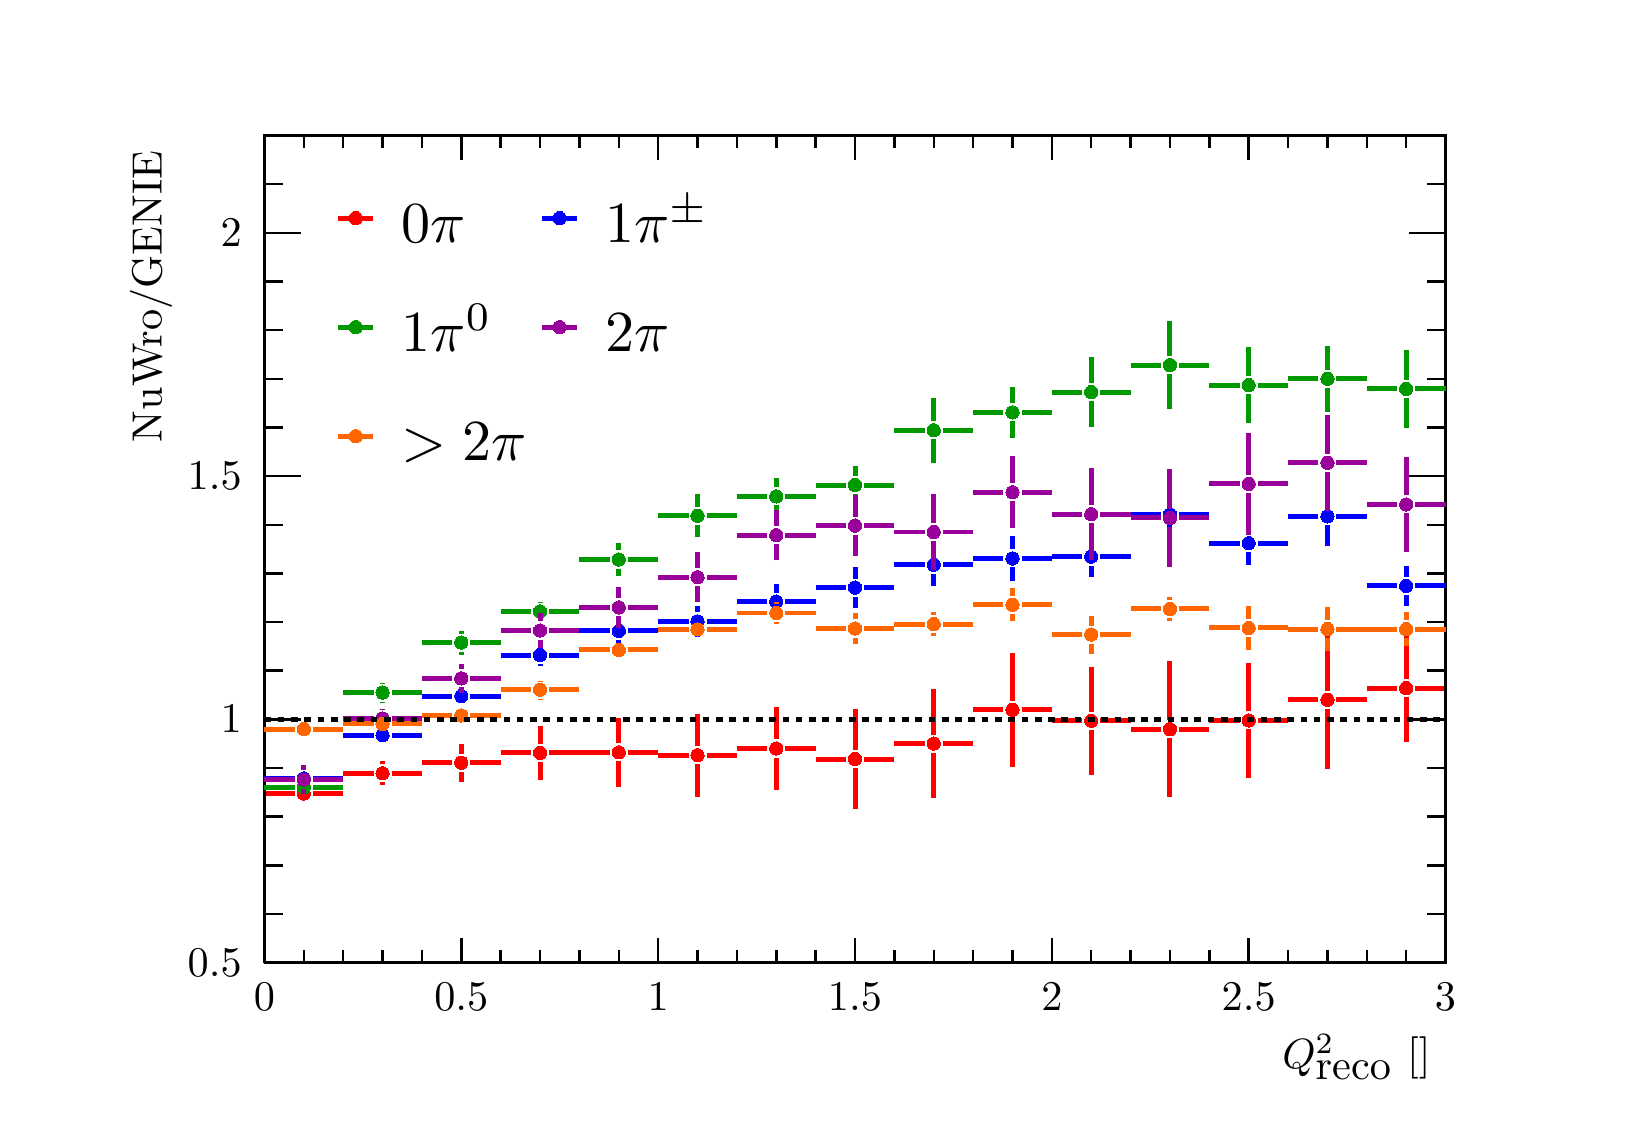
\begin{tikzpicture}
\pgfdeclareplotmark{cross} {
\pgfpathmoveto{\pgfpoint{-0.3\pgfplotmarksize}{\pgfplotmarksize}}
\pgfpathlineto{\pgfpoint{+0.3\pgfplotmarksize}{\pgfplotmarksize}}
\pgfpathlineto{\pgfpoint{+0.3\pgfplotmarksize}{0.3\pgfplotmarksize}}
\pgfpathlineto{\pgfpoint{+1\pgfplotmarksize}{0.3\pgfplotmarksize}}
\pgfpathlineto{\pgfpoint{+1\pgfplotmarksize}{-0.3\pgfplotmarksize}}
\pgfpathlineto{\pgfpoint{+0.3\pgfplotmarksize}{-0.3\pgfplotmarksize}}
\pgfpathlineto{\pgfpoint{+0.3\pgfplotmarksize}{-1.\pgfplotmarksize}}
\pgfpathlineto{\pgfpoint{-0.3\pgfplotmarksize}{-1.\pgfplotmarksize}}
\pgfpathlineto{\pgfpoint{-0.3\pgfplotmarksize}{-0.3\pgfplotmarksize}}
\pgfpathlineto{\pgfpoint{-1.\pgfplotmarksize}{-0.3\pgfplotmarksize}}
\pgfpathlineto{\pgfpoint{-1.\pgfplotmarksize}{0.3\pgfplotmarksize}}
\pgfpathlineto{\pgfpoint{-0.3\pgfplotmarksize}{0.3\pgfplotmarksize}}
\pgfpathclose
\pgfusepathqstroke
}
\pgfdeclareplotmark{cross*} {
\pgfpathmoveto{\pgfpoint{-0.3\pgfplotmarksize}{\pgfplotmarksize}}
\pgfpathlineto{\pgfpoint{+0.3\pgfplotmarksize}{\pgfplotmarksize}}
\pgfpathlineto{\pgfpoint{+0.3\pgfplotmarksize}{0.3\pgfplotmarksize}}
\pgfpathlineto{\pgfpoint{+1\pgfplotmarksize}{0.3\pgfplotmarksize}}
\pgfpathlineto{\pgfpoint{+1\pgfplotmarksize}{-0.3\pgfplotmarksize}}
\pgfpathlineto{\pgfpoint{+0.3\pgfplotmarksize}{-0.3\pgfplotmarksize}}
\pgfpathlineto{\pgfpoint{+0.3\pgfplotmarksize}{-1.\pgfplotmarksize}}
\pgfpathlineto{\pgfpoint{-0.3\pgfplotmarksize}{-1.\pgfplotmarksize}}
\pgfpathlineto{\pgfpoint{-0.3\pgfplotmarksize}{-0.3\pgfplotmarksize}}
\pgfpathlineto{\pgfpoint{-1.\pgfplotmarksize}{-0.3\pgfplotmarksize}}
\pgfpathlineto{\pgfpoint{-1.\pgfplotmarksize}{0.3\pgfplotmarksize}}
\pgfpathlineto{\pgfpoint{-0.3\pgfplotmarksize}{0.3\pgfplotmarksize}}
\pgfpathclose
\pgfusepathqfillstroke
}
\pgfdeclareplotmark{newstar} {
\pgfpathmoveto{\pgfqpoint{0pt}{\pgfplotmarksize}}
\pgfpathlineto{\pgfqpointpolar{44}{0.5\pgfplotmarksize}}
\pgfpathlineto{\pgfqpointpolar{18}{\pgfplotmarksize}}
\pgfpathlineto{\pgfqpointpolar{-20}{0.5\pgfplotmarksize}}
\pgfpathlineto{\pgfqpointpolar{-54}{\pgfplotmarksize}}
\pgfpathlineto{\pgfqpointpolar{-90}{0.5\pgfplotmarksize}}
\pgfpathlineto{\pgfqpointpolar{234}{\pgfplotmarksize}}
\pgfpathlineto{\pgfqpointpolar{198}{0.5\pgfplotmarksize}}
\pgfpathlineto{\pgfqpointpolar{162}{\pgfplotmarksize}}
\pgfpathlineto{\pgfqpointpolar{134}{0.5\pgfplotmarksize}}
\pgfpathclose
\pgfusepathqstroke
}
\pgfdeclareplotmark{newstar*} {
\pgfpathmoveto{\pgfqpoint{0pt}{\pgfplotmarksize}}
\pgfpathlineto{\pgfqpointpolar{44}{0.5\pgfplotmarksize}}
\pgfpathlineto{\pgfqpointpolar{18}{\pgfplotmarksize}}
\pgfpathlineto{\pgfqpointpolar{-20}{0.5\pgfplotmarksize}}
\pgfpathlineto{\pgfqpointpolar{-54}{\pgfplotmarksize}}
\pgfpathlineto{\pgfqpointpolar{-90}{0.5\pgfplotmarksize}}
\pgfpathlineto{\pgfqpointpolar{234}{\pgfplotmarksize}}
\pgfpathlineto{\pgfqpointpolar{198}{0.5\pgfplotmarksize}}
\pgfpathlineto{\pgfqpointpolar{162}{\pgfplotmarksize}}
\pgfpathlineto{\pgfqpointpolar{134}{0.5\pgfplotmarksize}}
\pgfpathclose
\pgfusepathqfillstroke
}
\definecolor{c}{rgb}{1,1,1};
\draw [color=c, fill=c] (0,0) rectangle (20,13.639);
\draw [color=c, fill=c] (3,1.77307) rectangle (18,12.2751);
\definecolor{c}{rgb}{0,0,0};
\draw [c,line width=0.9] (3,1.77307) -- (3,12.2751) -- (18,12.2751) -- (18,1.77307) -- (3,1.77307);
\definecolor{c}{rgb}{1,1,1};
\draw [color=c, fill=c] (3,1.77307) rectangle (18,12.2751);
\definecolor{c}{rgb}{0,0,0};
\draw [c,line width=0.9] (3,1.77307) -- (3,12.2751) -- (18,12.2751) -- (18,1.77307) -- (3,1.77307);
\definecolor{c}{rgb}{1,0,0};
\draw [c,line width=1.8] (3,3.91911) -- (3.38539,3.91911);
\draw [c,line width=1.8] (3.61461,3.91911) -- (4,3.91911);
\foreach \P in {(3.5,3.91911)}{\draw[mark options={color=c,fill=c},mark size=2.402402pt, line width=0.000000pt, mark=*] plot coordinates {\P};}
\draw [c,line width=1.8] (4.5,4.02491) -- (4.5,4.06197);
\draw [c,line width=1.8] (4.5,4.2912) -- (4.5,4.32827);
\draw [c,line width=1.8] (4,4.17659) -- (4.38539,4.17659);
\draw [c,line width=1.8] (4.61461,4.17659) -- (5,4.17659);
\foreach \P in {(4.5,4.17659)}{\draw[mark options={color=c,fill=c},mark size=2.402402pt, line width=0.000000pt, mark=*] plot coordinates {\P};}
\draw [c,line width=1.8] (5.5,4.06967) -- (5.5,4.19653);
\draw [c,line width=1.8] (5.5,4.42576) -- (5.5,4.55262);
\draw [c,line width=1.8] (5,4.31115) -- (5.38539,4.31115);
\draw [c,line width=1.8] (5.61461,4.31115) -- (6,4.31115);
\foreach \P in {(5.5,4.31115)}{\draw[mark options={color=c,fill=c},mark size=2.402402pt, line width=0.000000pt, mark=*] plot coordinates {\P};}
\draw [c,line width=1.8] (6.5,4.09054) -- (6.5,4.32215);
\draw [c,line width=1.8] (6.5,4.55138) -- (6.5,4.78299);
\draw [c,line width=1.8] (6,4.43676) -- (6.38539,4.43676);
\draw [c,line width=1.8] (6.61461,4.43676) -- (7,4.43676);
\foreach \P in {(6.5,4.43676)}{\draw[mark options={color=c,fill=c},mark size=2.402402pt, line width=0.000000pt, mark=*] plot coordinates {\P};}
\draw [c,line width=1.8] (7.5,4.00439) -- (7.5,4.32806);
\draw [c,line width=1.8] (7.5,4.55729) -- (7.5,4.88095);
\draw [c,line width=1.8] (7,4.44267) -- (7.38539,4.44267);
\draw [c,line width=1.8] (7.61461,4.44267) -- (8,4.44267);
\foreach \P in {(7.5,4.44267)}{\draw[mark options={color=c,fill=c},mark size=2.402402pt, line width=0.000000pt, mark=*] plot coordinates {\P};}
\draw [c,line width=1.8] (8.5,3.88168) -- (8.5,4.2921);
\draw [c,line width=1.8] (8.5,4.52133) -- (8.5,4.93175);
\draw [c,line width=1.8] (8,4.40671) -- (8.38539,4.40671);
\draw [c,line width=1.8] (8.61461,4.40671) -- (9,4.40671);
\foreach \P in {(8.5,4.40671)}{\draw[mark options={color=c,fill=c},mark size=2.402402pt, line width=0.000000pt, mark=*] plot coordinates {\P};}
\draw [c,line width=1.8] (9.5,3.95924) -- (9.5,4.37703);
\draw [c,line width=1.8] (9.5,4.60626) -- (9.5,5.02405);
\draw [c,line width=1.8] (9,4.49165) -- (9.38539,4.49165);
\draw [c,line width=1.8] (9.61461,4.49165) -- (10,4.49165);
\foreach \P in {(9.5,4.49165)}{\draw[mark options={color=c,fill=c},mark size=2.402402pt, line width=0.000000pt, mark=*] plot coordinates {\P};}
\draw [c,line width=1.8] (10.5,3.72077) -- (10.5,4.24284);
\draw [c,line width=1.8] (10.5,4.47207) -- (10.5,4.99414);
\draw [c,line width=1.8] (10,4.35746) -- (10.3854,4.35746);
\draw [c,line width=1.8] (10.6146,4.35746) -- (11,4.35746);
\foreach \P in {(10.5,4.35746)}{\draw[mark options={color=c,fill=c},mark size=2.402402pt, line width=0.000000pt, mark=*] plot coordinates {\P};}
\draw [c,line width=1.8] (11.5,3.86667) -- (11.5,4.43937);
\draw [c,line width=1.8] (11.5,4.6686) -- (11.5,5.24131);
\draw [c,line width=1.8] (11,4.55399) -- (11.3854,4.55399);
\draw [c,line width=1.8] (11.6146,4.55399) -- (12,4.55399);
\foreach \P in {(11.5,4.55399)}{\draw[mark options={color=c,fill=c},mark size=2.402402pt, line width=0.000000pt, mark=*] plot coordinates {\P};}
\draw [c,line width=1.8] (12.5,4.26285) -- (12.5,4.86913);
\draw [c,line width=1.8] (12.5,5.09835) -- (12.5,5.70464);
\draw [c,line width=1.8] (12,4.98374) -- (12.3854,4.98374);
\draw [c,line width=1.8] (12.6146,4.98374) -- (13,4.98374);
\foreach \P in {(12.5,4.98374)}{\draw[mark options={color=c,fill=c},mark size=2.402402pt, line width=0.000000pt, mark=*] plot coordinates {\P};}
\draw [c,line width=1.8] (13.5,4.16025) -- (13.5,4.72872);
\draw [c,line width=1.8] (13.5,4.95794) -- (13.5,5.52641);
\draw [c,line width=1.8] (13,4.84333) -- (13.3854,4.84333);
\draw [c,line width=1.8] (13.6146,4.84333) -- (14,4.84333);
\foreach \P in {(13.5,4.84333)}{\draw[mark options={color=c,fill=c},mark size=2.402402pt, line width=0.000000pt, mark=*] plot coordinates {\P};}
\draw [c,line width=1.8] (14.5,3.87445) -- (14.5,4.62216);
\draw [c,line width=1.8] (14.5,4.85139) -- (14.5,5.59911);
\draw [c,line width=1.8] (14,4.73678) -- (14.3854,4.73678);
\draw [c,line width=1.8] (14.6146,4.73678) -- (15,4.73678);
\foreach \P in {(14.5,4.73678)}{\draw[mark options={color=c,fill=c},mark size=2.402402pt, line width=0.000000pt, mark=*] plot coordinates {\P};}
\draw [c,line width=1.8] (15.5,4.12242) -- (15.5,4.73293);
\draw [c,line width=1.8] (15.5,4.96216) -- (15.5,5.57267);
\draw [c,line width=1.8] (15,4.84755) -- (15.3854,4.84755);
\draw [c,line width=1.8] (15.6146,4.84755) -- (16,4.84755);
\foreach \P in {(15.5,4.84755)}{\draw[mark options={color=c,fill=c},mark size=2.402402pt, line width=0.000000pt, mark=*] plot coordinates {\P};}
\draw [c,line width=1.8] (16.5,4.23132) -- (16.5,4.99592);
\draw [c,line width=1.8] (16.5,5.22515) -- (16.5,5.98976);
\draw [c,line width=1.8] (16,5.11054) -- (16.3854,5.11054);
\draw [c,line width=1.8] (16.6146,5.11054) -- (17,5.11054);
\foreach \P in {(16.5,5.11054)}{\draw[mark options={color=c,fill=c},mark size=2.402402pt, line width=0.000000pt, mark=*] plot coordinates {\P};}
\draw [c,line width=1.8] (17.5,4.57864) -- (17.5,5.14441);
\draw [c,line width=1.8] (17.5,5.37364) -- (17.5,5.93942);
\draw [c,line width=1.8] (17,5.25903) -- (17.3854,5.25903);
\draw [c,line width=1.8] (17.6146,5.25903) -- (18,5.25903);
\foreach \P in {(17.5,5.25903)}{\draw[mark options={color=c,fill=c},mark size=2.402402pt, line width=0.000000pt, mark=*] plot coordinates {\P};}
\definecolor{c}{rgb}{0,0,0};
\draw [c,line width=0.9] (3,1.77307) -- (18,1.77307);
\draw [c,line width=0.9] (3,2.07994) -- (3,1.77307);
\draw [c,line width=0.9] (3.5,1.9265) -- (3.5,1.77307);
\draw [c,line width=0.9] (4,1.9265) -- (4,1.77307);
\draw [c,line width=0.9] (4.5,1.9265) -- (4.5,1.77307);
\draw [c,line width=0.9] (5,1.9265) -- (5,1.77307);
\draw [c,line width=0.9] (5.5,2.07994) -- (5.5,1.77307);
\draw [c,line width=0.9] (6,1.9265) -- (6,1.77307);
\draw [c,line width=0.9] (6.5,1.9265) -- (6.5,1.77307);
\draw [c,line width=0.9] (7,1.9265) -- (7,1.77307);
\draw [c,line width=0.9] (7.5,1.9265) -- (7.5,1.77307);
\draw [c,line width=0.9] (8,2.07994) -- (8,1.77307);
\draw [c,line width=0.9] (8.5,1.9265) -- (8.5,1.77307);
\draw [c,line width=0.9] (9,1.9265) -- (9,1.77307);
\draw [c,line width=0.9] (9.5,1.9265) -- (9.5,1.77307);
\draw [c,line width=0.9] (10,1.9265) -- (10,1.77307);
\draw [c,line width=0.9] (10.5,2.07994) -- (10.5,1.77307);
\draw [c,line width=0.9] (11,1.9265) -- (11,1.77307);
\draw [c,line width=0.9] (11.5,1.9265) -- (11.5,1.77307);
\draw [c,line width=0.9] (12,1.9265) -- (12,1.77307);
\draw [c,line width=0.9] (12.5,1.9265) -- (12.5,1.77307);
\draw [c,line width=0.9] (13,2.07994) -- (13,1.77307);
\draw [c,line width=0.9] (13.5,1.9265) -- (13.5,1.77307);
\draw [c,line width=0.9] (14,1.9265) -- (14,1.77307);
\draw [c,line width=0.9] (14.5,1.9265) -- (14.5,1.77307);
\draw [c,line width=0.9] (15,1.9265) -- (15,1.77307);
\draw [c,line width=0.9] (15.5,2.07994) -- (15.5,1.77307);
\draw [c,line width=0.9] (16,1.9265) -- (16,1.77307);
\draw [c,line width=0.9] (16.5,1.9265) -- (16.5,1.77307);
\draw [c,line width=0.9] (17,1.9265) -- (17,1.77307);
\draw [c,line width=0.9] (17.5,1.9265) -- (17.5,1.77307);
\draw [c,line width=0.9] (18,2.07994) -- (18,1.77307);
\draw [c,line width=0.9] (18,2.07994) -- (18,1.77307);
\draw [anchor=base] (3,1.15931) node[scale=1.52731, color=c, rotate=0]{0};
\draw [anchor=base] (5.5,1.15931) node[scale=1.52731, color=c, rotate=0]{0.5};
\draw [anchor=base] (8,1.15931) node[scale=1.52731, color=c, rotate=0]{1};
\draw [anchor=base] (10.5,1.15931) node[scale=1.52731, color=c, rotate=0]{1.5};
\draw [anchor=base] (13,1.15931) node[scale=1.52731, color=c, rotate=0]{2};
\draw [anchor=base] (15.5,1.15931) node[scale=1.52731, color=c, rotate=0]{2.5};
\draw [anchor=base] (18,1.15931) node[scale=1.52731, color=c, rotate=0]{3};
\draw [anchor= east] (18,0.572837) node[scale=1.52731, color=c, rotate=0]{$Q^{2}_{\textrm{reco}}$ [\si{\GeV\squared}] };
\draw [c,line width=0.9] (3,12.2751) -- (18,12.2751);
\draw [c,line width=0.9] (3,11.9682) -- (3,12.2751);
\draw [c,line width=0.9] (3.5,12.1216) -- (3.5,12.2751);
\draw [c,line width=0.9] (4,12.1216) -- (4,12.2751);
\draw [c,line width=0.9] (4.5,12.1216) -- (4.5,12.2751);
\draw [c,line width=0.9] (5,12.1216) -- (5,12.2751);
\draw [c,line width=0.9] (5.5,11.9682) -- (5.5,12.2751);
\draw [c,line width=0.9] (6,12.1216) -- (6,12.2751);
\draw [c,line width=0.9] (6.5,12.1216) -- (6.5,12.2751);
\draw [c,line width=0.9] (7,12.1216) -- (7,12.2751);
\draw [c,line width=0.9] (7.5,12.1216) -- (7.5,12.2751);
\draw [c,line width=0.9] (8,11.9682) -- (8,12.2751);
\draw [c,line width=0.9] (8.5,12.1216) -- (8.5,12.2751);
\draw [c,line width=0.9] (9,12.1216) -- (9,12.2751);
\draw [c,line width=0.9] (9.5,12.1216) -- (9.5,12.2751);
\draw [c,line width=0.9] (10,12.1216) -- (10,12.2751);
\draw [c,line width=0.9] (10.5,11.9682) -- (10.5,12.2751);
\draw [c,line width=0.9] (11,12.1216) -- (11,12.2751);
\draw [c,line width=0.9] (11.5,12.1216) -- (11.5,12.2751);
\draw [c,line width=0.9] (12,12.1216) -- (12,12.2751);
\draw [c,line width=0.9] (12.5,12.1216) -- (12.5,12.2751);
\draw [c,line width=0.9] (13,11.9682) -- (13,12.2751);
\draw [c,line width=0.9] (13.5,12.1216) -- (13.5,12.2751);
\draw [c,line width=0.9] (14,12.1216) -- (14,12.2751);
\draw [c,line width=0.9] (14.5,12.1216) -- (14.5,12.2751);
\draw [c,line width=0.9] (15,12.1216) -- (15,12.2751);
\draw [c,line width=0.9] (15.5,11.9682) -- (15.5,12.2751);
\draw [c,line width=0.9] (16,12.1216) -- (16,12.2751);
\draw [c,line width=0.9] (16.5,12.1216) -- (16.5,12.2751);
\draw [c,line width=0.9] (17,12.1216) -- (17,12.2751);
\draw [c,line width=0.9] (17.5,12.1216) -- (17.5,12.2751);
\draw [c,line width=0.9] (18,11.9682) -- (18,12.2751);
\draw [c,line width=0.9] (18,11.9682) -- (18,12.2751);
\draw [c,line width=0.9] (3,1.77307) -- (3,12.2751);
\draw [c,line width=0.9] (3.462,1.77307) -- (3,1.77307);
\draw [c,line width=0.9] (3.231,2.39083) -- (3,2.39083);
\draw [c,line width=0.9] (3.231,3.0086) -- (3,3.0086);
\draw [c,line width=0.9] (3.231,3.62636) -- (3,3.62636);
\draw [c,line width=0.9] (3.231,4.24413) -- (3,4.24413);
\draw [c,line width=0.9] (3.462,4.86189) -- (3,4.86189);
\draw [c,line width=0.9] (3.231,5.47966) -- (3,5.47966);
\draw [c,line width=0.9] (3.231,6.09742) -- (3,6.09742);
\draw [c,line width=0.9] (3.231,6.71519) -- (3,6.71519);
\draw [c,line width=0.9] (3.231,7.33295) -- (3,7.33295);
\draw [c,line width=0.9] (3.462,7.95072) -- (3,7.95072);
\draw [c,line width=0.9] (3.231,8.56848) -- (3,8.56848);
\draw [c,line width=0.9] (3.231,9.18625) -- (3,9.18625);
\draw [c,line width=0.9] (3.231,9.80401) -- (3,9.80401);
\draw [c,line width=0.9] (3.231,10.4218) -- (3,10.4218);
\draw [c,line width=0.9] (3.462,11.0395) -- (3,11.0395);
\draw [c,line width=0.9] (3.462,11.0395) -- (3,11.0395);
\draw [c,line width=0.9] (3.231,11.6573) -- (3,11.6573);
\draw [c,line width=0.9] (3.231,12.2751) -- (3,12.2751);
\draw [anchor= east] (2.9,1.77307) node[scale=1.52731, color=c, rotate=0]{0.5};
\draw [anchor= east] (2.9,4.86189) node[scale=1.52731, color=c, rotate=0]{1};
\draw [anchor= east] (2.9,7.95072) node[scale=1.52731, color=c, rotate=0]{1.5};
\draw [anchor= east] (2.9,11.0395) node[scale=1.52731, color=c, rotate=0]{2};
\draw [anchor= east] (1.56,12.2751) node[scale=1.52731, color=c, rotate=90]{ NuWro/GENIE};
\draw [c,line width=0.9] (18,1.77307) -- (18,12.2751);
\draw [c,line width=0.9] (17.538,1.77307) -- (18,1.77307);
\draw [c,line width=0.9] (17.769,2.39083) -- (18,2.39083);
\draw [c,line width=0.9] (17.769,3.0086) -- (18,3.0086);
\draw [c,line width=0.9] (17.769,3.62636) -- (18,3.62636);
\draw [c,line width=0.9] (17.769,4.24413) -- (18,4.24413);
\draw [c,line width=0.9] (17.538,4.86189) -- (18,4.86189);
\draw [c,line width=0.9] (17.769,5.47966) -- (18,5.47966);
\draw [c,line width=0.9] (17.769,6.09742) -- (18,6.09742);
\draw [c,line width=0.9] (17.769,6.71519) -- (18,6.71519);
\draw [c,line width=0.9] (17.769,7.33295) -- (18,7.33295);
\draw [c,line width=0.9] (17.538,7.95072) -- (18,7.95072);
\draw [c,line width=0.9] (17.769,8.56848) -- (18,8.56848);
\draw [c,line width=0.9] (17.769,9.18625) -- (18,9.18625);
\draw [c,line width=0.9] (17.769,9.80401) -- (18,9.80401);
\draw [c,line width=0.9] (17.769,10.4218) -- (18,10.4218);
\draw [c,line width=0.9] (17.538,11.0395) -- (18,11.0395);
\draw [c,line width=0.9] (17.538,11.0395) -- (18,11.0395);
\draw [c,line width=0.9] (17.769,11.6573) -- (18,11.6573);
\draw [c,line width=0.9] (17.769,12.2751) -- (18,12.2751);
\definecolor{c}{rgb}{0,0,1};
\draw [c,line width=1.8] (3,4.11165) -- (3.38539,4.11165);
\draw [c,line width=1.8] (3.61461,4.11165) -- (4,4.11165);
\foreach \P in {(3.5,4.11165)}{\draw[mark options={color=c,fill=c},mark size=2.402402pt, line width=0.000000pt, mark=*] plot coordinates {\P};}
\draw [c,line width=1.8] (4,4.66109) -- (4.38539,4.66109);
\draw [c,line width=1.8] (4.61461,4.66109) -- (5,4.66109);
\foreach \P in {(4.5,4.66109)}{\draw[mark options={color=c,fill=c},mark size=2.402402pt, line width=0.000000pt, mark=*] plot coordinates {\P};}
\draw [c,line width=1.8] (5,5.15734) -- (5.38539,5.15734);
\draw [c,line width=1.8] (5.61461,5.15734) -- (6,5.15734);
\foreach \P in {(5.5,5.15734)}{\draw[mark options={color=c,fill=c},mark size=2.402402pt, line width=0.000000pt, mark=*] plot coordinates {\P};}
\draw [c,line width=1.8] (6.5,5.53786) -- (6.5,5.5637);
\draw [c,line width=1.8] (6.5,5.79293) -- (6.5,5.81878);
\draw [c,line width=1.8] (6,5.67832) -- (6.38539,5.67832);
\draw [c,line width=1.8] (6.61461,5.67832) -- (7,5.67832);
\foreach \P in {(6.5,5.67832)}{\draw[mark options={color=c,fill=c},mark size=2.402402pt, line width=0.000000pt, mark=*] plot coordinates {\P};}
\draw [c,line width=1.8] (7.5,5.81405) -- (7.5,5.87022);
\draw [c,line width=1.8] (7.5,6.09945) -- (7.5,6.15562);
\draw [c,line width=1.8] (7,5.98483) -- (7.38539,5.98483);
\draw [c,line width=1.8] (7.61461,5.98483) -- (8,5.98483);
\foreach \P in {(7.5,5.98483)}{\draw[mark options={color=c,fill=c},mark size=2.402402pt, line width=0.000000pt, mark=*] plot coordinates {\P};}
\draw [c,line width=1.8] (8.5,5.90476) -- (8.5,5.99085);
\draw [c,line width=1.8] (8.5,6.22008) -- (8.5,6.30618);
\draw [c,line width=1.8] (8,6.10547) -- (8.38539,6.10547);
\draw [c,line width=1.8] (8.61461,6.10547) -- (9,6.10547);
\foreach \P in {(8.5,6.10547)}{\draw[mark options={color=c,fill=c},mark size=2.402402pt, line width=0.000000pt, mark=*] plot coordinates {\P};}
\draw [c,line width=1.8] (9.5,6.13423) -- (9.5,6.2426);
\draw [c,line width=1.8] (9.5,6.47183) -- (9.5,6.58021);
\draw [c,line width=1.8] (9,6.35722) -- (9.38539,6.35722);
\draw [c,line width=1.8] (9.61461,6.35722) -- (10,6.35722);
\foreach \P in {(9.5,6.35722)}{\draw[mark options={color=c,fill=c},mark size=2.402402pt, line width=0.000000pt, mark=*] plot coordinates {\P};}
\draw [c,line width=1.8] (10.5,6.27812) -- (10.5,6.42058);
\draw [c,line width=1.8] (10.5,6.64981) -- (10.5,6.79227);
\draw [c,line width=1.8] (10,6.53519) -- (10.3854,6.53519);
\draw [c,line width=1.8] (10.6146,6.53519) -- (11,6.53519);
\foreach \P in {(10.5,6.53519)}{\draw[mark options={color=c,fill=c},mark size=2.402402pt, line width=0.000000pt, mark=*] plot coordinates {\P};}
\draw [c,line width=1.8] (11.5,6.55622) -- (11.5,6.71101);
\draw [c,line width=1.8] (11.5,6.94024) -- (11.5,7.09502);
\draw [c,line width=1.8] (11,6.82562) -- (11.3854,6.82562);
\draw [c,line width=1.8] (11.6146,6.82562) -- (12,6.82562);
\foreach \P in {(11.5,6.82562)}{\draw[mark options={color=c,fill=c},mark size=2.402402pt, line width=0.000000pt, mark=*] plot coordinates {\P};}
\draw [c,line width=1.8] (12.5,6.62113) -- (12.5,6.79021);
\draw [c,line width=1.8] (12.5,7.01944) -- (12.5,7.18851);
\draw [c,line width=1.8] (12,6.90482) -- (12.3854,6.90482);
\draw [c,line width=1.8] (12.6146,6.90482) -- (13,6.90482);
\foreach \P in {(12.5,6.90482)}{\draw[mark options={color=c,fill=c},mark size=2.402402pt, line width=0.000000pt, mark=*] plot coordinates {\P};}
\draw [c,line width=1.8] (13.5,6.67157) -- (13.5,6.81355);
\draw [c,line width=1.8] (13.5,7.04278) -- (13.5,7.18476);
\draw [c,line width=1.8] (13,6.92817) -- (13.3854,6.92817);
\draw [c,line width=1.8] (13.6146,6.92817) -- (14,6.92817);
\foreach \P in {(13.5,6.92817)}{\draw[mark options={color=c,fill=c},mark size=2.402402pt, line width=0.000000pt, mark=*] plot coordinates {\P};}
\draw [c,line width=1.8] (14.5,7.0792) -- (14.5,7.34926);
\draw [c,line width=1.8] (14.5,7.57849) -- (14.5,7.84855);
\draw [c,line width=1.8] (14,7.46388) -- (14.3854,7.46388);
\draw [c,line width=1.8] (14.6146,7.46388) -- (15,7.46388);
\foreach \P in {(14.5,7.46388)}{\draw[mark options={color=c,fill=c},mark size=2.402402pt, line width=0.000000pt, mark=*] plot coordinates {\P};}
\draw [c,line width=1.8] (15.5,6.82626) -- (15.5,6.98466);
\draw [c,line width=1.8] (15.5,7.21389) -- (15.5,7.37229);
\draw [c,line width=1.8] (15,7.09927) -- (15.3854,7.09927);
\draw [c,line width=1.8] (15.6146,7.09927) -- (16,7.09927);
\foreach \P in {(15.5,7.09927)}{\draw[mark options={color=c,fill=c},mark size=2.402402pt, line width=0.000000pt, mark=*] plot coordinates {\P};}
\draw [c,line width=1.8] (16.5,7.06422) -- (16.5,7.32444);
\draw [c,line width=1.8] (16.5,7.55366) -- (16.5,7.81388);
\draw [c,line width=1.8] (16,7.43905) -- (16.3854,7.43905);
\draw [c,line width=1.8] (16.6146,7.43905) -- (17,7.43905);
\foreach \P in {(16.5,7.43905)}{\draw[mark options={color=c,fill=c},mark size=2.402402pt, line width=0.000000pt, mark=*] plot coordinates {\P};}
\draw [c,line width=1.8] (17.5,6.30612) -- (17.5,6.44302);
\draw [c,line width=1.8] (17.5,6.67224) -- (17.5,6.80914);
\draw [c,line width=1.8] (17,6.55763) -- (17.3854,6.55763);
\draw [c,line width=1.8] (17.6146,6.55763) -- (18,6.55763);
\foreach \P in {(17.5,6.55763)}{\draw[mark options={color=c,fill=c},mark size=2.402402pt, line width=0.000000pt, mark=*] plot coordinates {\P};}
\definecolor{c}{rgb}{0,0.6,0};
\draw [c,line width=1.8] (3,4.00063) -- (3.38539,4.00063);
\draw [c,line width=1.8] (3.61461,4.00063) -- (4,4.00063);
\foreach \P in {(3.5,4.00063)}{\draw[mark options={color=c,fill=c},mark size=2.402402pt, line width=0.000000pt, mark=*] plot coordinates {\P};}
\draw [c,line width=1.8] (4.5,5.08587) -- (4.5,5.08748);
\draw [c,line width=1.8] (4.5,5.31671) -- (4.5,5.31831);
\draw [c,line width=1.8] (4,5.20209) -- (4.38539,5.20209);
\draw [c,line width=1.8] (4.61461,5.20209) -- (5,5.20209);
\foreach \P in {(4.5,5.20209)}{\draw[mark options={color=c,fill=c},mark size=2.402402pt, line width=0.000000pt, mark=*] plot coordinates {\P};}
\draw [c,line width=1.8] (5.5,5.6837) -- (5.5,5.72221);
\draw [c,line width=1.8] (5.5,5.95144) -- (5.5,5.98995);
\draw [c,line width=1.8] (5,5.83682) -- (5.38539,5.83682);
\draw [c,line width=1.8] (5.61461,5.83682) -- (6,5.83682);
\foreach \P in {(5.5,5.83682)}{\draw[mark options={color=c,fill=c},mark size=2.402402pt, line width=0.000000pt, mark=*] plot coordinates {\P};}
\draw [c,line width=1.8] (6.5,6.11477) -- (6.5,6.11856);
\draw [c,line width=1.8] (6.5,6.34778) -- (6.5,6.35157);
\draw [c,line width=1.8] (6,6.23317) -- (6.38539,6.23317);
\draw [c,line width=1.8] (6.61461,6.23317) -- (7,6.23317);
\foreach \P in {(6.5,6.23317)}{\draw[mark options={color=c,fill=c},mark size=2.402402pt, line width=0.000000pt, mark=*] plot coordinates {\P};}
\draw [c,line width=1.8] (7.5,6.67663) -- (7.5,6.77696);
\draw [c,line width=1.8] (7.5,7.00619) -- (7.5,7.10653);
\draw [c,line width=1.8] (7,6.89158) -- (7.38539,6.89158);
\draw [c,line width=1.8] (7.61461,6.89158) -- (8,6.89158);
\foreach \P in {(7.5,6.89158)}{\draw[mark options={color=c,fill=c},mark size=2.402402pt, line width=0.000000pt, mark=*] plot coordinates {\P};}
\draw [c,line width=1.8] (8.5,7.17253) -- (8.5,7.33205);
\draw [c,line width=1.8] (8.5,7.56127) -- (8.5,7.72078);
\draw [c,line width=1.8] (8,7.44666) -- (8.38539,7.44666);
\draw [c,line width=1.8] (8.61461,7.44666) -- (9,7.44666);
\foreach \P in {(8.5,7.44666)}{\draw[mark options={color=c,fill=c},mark size=2.402402pt, line width=0.000000pt, mark=*] plot coordinates {\P};}
\draw [c,line width=1.8] (9.5,7.46544) -- (9.5,7.57908);
\draw [c,line width=1.8] (9.5,7.8083) -- (9.5,7.92194);
\draw [c,line width=1.8] (9,7.69369) -- (9.38539,7.69369);
\draw [c,line width=1.8] (9.61461,7.69369) -- (10,7.69369);
\foreach \P in {(9.5,7.69369)}{\draw[mark options={color=c,fill=c},mark size=2.402402pt, line width=0.000000pt, mark=*] plot coordinates {\P};}
\draw [c,line width=1.8] (10.5,7.5936) -- (10.5,7.72286);
\draw [c,line width=1.8] (10.5,7.95209) -- (10.5,8.08135);
\draw [c,line width=1.8] (10,7.83748) -- (10.3854,7.83748);
\draw [c,line width=1.8] (10.6146,7.83748) -- (11,7.83748);
\foreach \P in {(10.5,7.83748)}{\draw[mark options={color=c,fill=c},mark size=2.402402pt, line width=0.000000pt, mark=*] plot coordinates {\P};}
\draw [c,line width=1.8] (11.5,8.11736) -- (11.5,8.41826);
\draw [c,line width=1.8] (11.5,8.64749) -- (11.5,8.9484);
\draw [c,line width=1.8] (11,8.53288) -- (11.3854,8.53288);
\draw [c,line width=1.8] (11.6146,8.53288) -- (12,8.53288);
\foreach \P in {(11.5,8.53288)}{\draw[mark options={color=c,fill=c},mark size=2.402402pt, line width=0.000000pt, mark=*] plot coordinates {\P};}
\draw [c,line width=1.8] (12.5,8.43939) -- (12.5,8.64546);
\draw [c,line width=1.8] (12.5,8.87468) -- (12.5,9.08075);
\draw [c,line width=1.8] (12,8.76007) -- (12.3854,8.76007);
\draw [c,line width=1.8] (12.6146,8.76007) -- (13,8.76007);
\foreach \P in {(12.5,8.76007)}{\draw[mark options={color=c,fill=c},mark size=2.402402pt, line width=0.000000pt, mark=*] plot coordinates {\P};}
\draw [c,line width=1.8] (13.5,8.57217) -- (13.5,8.90391);
\draw [c,line width=1.8] (13.5,9.13314) -- (13.5,9.46488);
\draw [c,line width=1.8] (13,9.01853) -- (13.3854,9.01853);
\draw [c,line width=1.8] (13.6146,9.01853) -- (14,9.01853);
\foreach \P in {(13.5,9.01853)}{\draw[mark options={color=c,fill=c},mark size=2.402402pt, line width=0.000000pt, mark=*] plot coordinates {\P};}
\draw [c,line width=1.8] (14.5,8.80553) -- (14.5,9.24543);
\draw [c,line width=1.8] (14.5,9.47466) -- (14.5,9.91457);
\draw [c,line width=1.8] (14,9.36005) -- (14.3854,9.36005);
\draw [c,line width=1.8] (14.6146,9.36005) -- (15,9.36005);
\foreach \P in {(14.5,9.36005)}{\draw[mark options={color=c,fill=c},mark size=2.402402pt, line width=0.000000pt, mark=*] plot coordinates {\P};}
\draw [c,line width=1.8] (15.5,8.62774) -- (15.5,8.99202);
\draw [c,line width=1.8] (15.5,9.22125) -- (15.5,9.58553);
\draw [c,line width=1.8] (15,9.10663) -- (15.3854,9.10663);
\draw [c,line width=1.8] (15.6146,9.10663) -- (16,9.10663);
\foreach \P in {(15.5,9.10663)}{\draw[mark options={color=c,fill=c},mark size=2.402402pt, line width=0.000000pt, mark=*] plot coordinates {\P};}
\draw [c,line width=1.8] (16.5,8.76744) -- (16.5,9.07229);
\draw [c,line width=1.8] (16.5,9.30151) -- (16.5,9.60636);
\draw [c,line width=1.8] (16,9.1869) -- (16.3854,9.1869);
\draw [c,line width=1.8] (16.6146,9.1869) -- (17,9.1869);
\foreach \P in {(16.5,9.1869)}{\draw[mark options={color=c,fill=c},mark size=2.402402pt, line width=0.000000pt, mark=*] plot coordinates {\P};}
\draw [c,line width=1.8] (17.5,8.56739) -- (17.5,8.94352);
\draw [c,line width=1.8] (17.5,9.17275) -- (17.5,9.54888);
\draw [c,line width=1.8] (17,9.05814) -- (17.3854,9.05814);
\draw [c,line width=1.8] (17.6146,9.05814) -- (18,9.05814);
\foreach \P in {(17.5,9.05814)}{\draw[mark options={color=c,fill=c},mark size=2.402402pt, line width=0.000000pt, mark=*] plot coordinates {\P};}
\definecolor{c}{rgb}{0.6,0,0.6};
\draw [c,line width=1.8] (3.5,3.91998) -- (3.5,3.98335);
\draw [c,line width=1.8] (3.5,4.21258) -- (3.5,4.27595);
\draw [c,line width=1.8] (3,4.09797) -- (3.38539,4.09797);
\draw [c,line width=1.8] (3.61461,4.09797) -- (4,4.09797);
\foreach \P in {(3.5,4.09797)}{\draw[mark options={color=c,fill=c},mark size=2.402402pt, line width=0.000000pt, mark=*] plot coordinates {\P};}
\draw [c,line width=1.8] (4.5,4.75095) -- (4.5,4.7568);
\draw [c,line width=1.8] (4.5,4.98603) -- (4.5,4.99189);
\draw [c,line width=1.8] (4,4.87142) -- (4.38539,4.87142);
\draw [c,line width=1.8] (4.61461,4.87142) -- (5,4.87142);
\foreach \P in {(4.5,4.87142)}{\draw[mark options={color=c,fill=c},mark size=2.402402pt, line width=0.000000pt, mark=*] plot coordinates {\P};}
\draw [c,line width=1.8] (5.5,5.20189) -- (5.5,5.26748);
\draw [c,line width=1.8] (5.5,5.4967) -- (5.5,5.56229);
\draw [c,line width=1.8] (5,5.38209) -- (5.38539,5.38209);
\draw [c,line width=1.8] (5.61461,5.38209) -- (6,5.38209);
\foreach \P in {(5.5,5.38209)}{\draw[mark options={color=c,fill=c},mark size=2.402402pt, line width=0.000000pt, mark=*] plot coordinates {\P};}
\draw [c,line width=1.8] (6.5,5.77335) -- (6.5,5.87562);
\draw [c,line width=1.8] (6.5,6.10484) -- (6.5,6.20711);
\draw [c,line width=1.8] (6,5.99023) -- (6.38539,5.99023);
\draw [c,line width=1.8] (6.61461,5.99023) -- (7,5.99023);
\foreach \P in {(6.5,5.99023)}{\draw[mark options={color=c,fill=c},mark size=2.402402pt, line width=0.000000pt, mark=*] plot coordinates {\P};}
\draw [c,line width=1.8] (7.5,6.01918) -- (7.5,6.16879);
\draw [c,line width=1.8] (7.5,6.39802) -- (7.5,6.54763);
\draw [c,line width=1.8] (7,6.28341) -- (7.38539,6.28341);
\draw [c,line width=1.8] (7.61461,6.28341) -- (8,6.28341);
\foreach \P in {(7.5,6.28341)}{\draw[mark options={color=c,fill=c},mark size=2.402402pt, line width=0.000000pt, mark=*] plot coordinates {\P};}
\draw [c,line width=1.8] (8.5,6.35054) -- (8.5,6.55266);
\draw [c,line width=1.8] (8.5,6.78188) -- (8.5,6.98401);
\draw [c,line width=1.8] (8,6.66727) -- (8.38539,6.66727);
\draw [c,line width=1.8] (8.61461,6.66727) -- (9,6.66727);
\foreach \P in {(8.5,6.66727)}{\draw[mark options={color=c,fill=c},mark size=2.402402pt, line width=0.000000pt, mark=*] plot coordinates {\P};}
\draw [c,line width=1.8] (9.5,6.88525) -- (9.5,7.08656);
\draw [c,line width=1.8] (9.5,7.31579) -- (9.5,7.51711);
\draw [c,line width=1.8] (9,7.20118) -- (9.38539,7.20118);
\draw [c,line width=1.8] (9.61461,7.20118) -- (10,7.20118);
\foreach \P in {(9.5,7.20118)}{\draw[mark options={color=c,fill=c},mark size=2.402402pt, line width=0.000000pt, mark=*] plot coordinates {\P};}
\draw [c,line width=1.8] (10.5,6.9329) -- (10.5,7.20765);
\draw [c,line width=1.8] (10.5,7.43687) -- (10.5,7.71162);
\draw [c,line width=1.8] (10,7.32226) -- (10.3854,7.32226);
\draw [c,line width=1.8] (10.6146,7.32226) -- (11,7.32226);
\foreach \P in {(10.5,7.32226)}{\draw[mark options={color=c,fill=c},mark size=2.402402pt, line width=0.000000pt, mark=*] plot coordinates {\P};}
\draw [c,line width=1.8] (11.5,6.75326) -- (11.5,7.12633);
\draw [c,line width=1.8] (11.5,7.35555) -- (11.5,7.72862);
\draw [c,line width=1.8] (11,7.24094) -- (11.3854,7.24094);
\draw [c,line width=1.8] (11.6146,7.24094) -- (12,7.24094);
\foreach \P in {(11.5,7.24094)}{\draw[mark options={color=c,fill=c},mark size=2.402402pt, line width=0.000000pt, mark=*] plot coordinates {\P};}
\draw [c,line width=1.8] (12.5,7.28836) -- (12.5,7.63171);
\draw [c,line width=1.8] (12.5,7.86094) -- (12.5,8.20429);
\draw [c,line width=1.8] (12,7.74633) -- (12.3854,7.74633);
\draw [c,line width=1.8] (12.6146,7.74633) -- (13,7.74633);
\foreach \P in {(12.5,7.74633)}{\draw[mark options={color=c,fill=c},mark size=2.402402pt, line width=0.000000pt, mark=*] plot coordinates {\P};}
\draw [c,line width=1.8] (13.5,6.88059) -- (13.5,7.35249);
\draw [c,line width=1.8] (13.5,7.58172) -- (13.5,8.05362);
\draw [c,line width=1.8] (13,7.4671) -- (13.3854,7.4671);
\draw [c,line width=1.8] (13.6146,7.4671) -- (14,7.4671);
\foreach \P in {(13.5,7.4671)}{\draw[mark options={color=c,fill=c},mark size=2.402402pt, line width=0.000000pt, mark=*] plot coordinates {\P};}
\draw [c,line width=1.8] (14.5,6.80071) -- (14.5,7.30545);
\draw [c,line width=1.8] (14.5,7.53468) -- (14.5,8.03941);
\draw [c,line width=1.8] (14,7.42006) -- (14.3854,7.42006);
\draw [c,line width=1.8] (14.6146,7.42006) -- (15,7.42006);
\foreach \P in {(14.5,7.42006)}{\draw[mark options={color=c,fill=c},mark size=2.402402pt, line width=0.000000pt, mark=*] plot coordinates {\P};}
\draw [c,line width=1.8] (15.5,7.20405) -- (15.5,7.73769);
\draw [c,line width=1.8] (15.5,7.96691) -- (15.5,8.50055);
\draw [c,line width=1.8] (15,7.8523) -- (15.3854,7.8523);
\draw [c,line width=1.8] (15.6146,7.8523) -- (16,7.8523);
\foreach \P in {(15.5,7.8523)}{\draw[mark options={color=c,fill=c},mark size=2.402402pt, line width=0.000000pt, mark=*] plot coordinates {\P};}
\draw [c,line width=1.8] (16.5,7.50909) -- (16.5,8.00597);
\draw [c,line width=1.8] (16.5,8.2352) -- (16.5,8.73207);
\draw [c,line width=1.8] (16,8.12058) -- (16.3854,8.12058);
\draw [c,line width=1.8] (16.6146,8.12058) -- (17,8.12058);
\foreach \P in {(16.5,8.12058)}{\draw[mark options={color=c,fill=c},mark size=2.402402pt, line width=0.000000pt, mark=*] plot coordinates {\P};}
\draw [c,line width=1.8] (17.5,6.9893) -- (17.5,7.4765);
\draw [c,line width=1.8] (17.5,7.70573) -- (17.5,8.19294);
\draw [c,line width=1.8] (17,7.59112) -- (17.3854,7.59112);
\draw [c,line width=1.8] (17.6146,7.59112) -- (18,7.59112);
\foreach \P in {(17.5,7.59112)}{\draw[mark options={color=c,fill=c},mark size=2.402402pt, line width=0.000000pt, mark=*] plot coordinates {\P};}
\definecolor{c}{rgb}{1,0.4,0};
\draw [c,line width=1.8] (3,4.73881) -- (3.38539,4.73881);
\draw [c,line width=1.8] (3.61461,4.73881) -- (4,4.73881);
\foreach \P in {(3.5,4.73881)}{\draw[mark options={color=c,fill=c},mark size=2.402402pt, line width=0.000000pt, mark=*] plot coordinates {\P};}
\draw [c,line width=1.8] (4,4.8038) -- (4.38539,4.8038);
\draw [c,line width=1.8] (4.61461,4.8038) -- (5,4.8038);
\foreach \P in {(4.5,4.8038)}{\draw[mark options={color=c,fill=c},mark size=2.402402pt, line width=0.000000pt, mark=*] plot coordinates {\P};}
\draw [c,line width=1.8] (5,4.9114) -- (5.38539,4.9114);
\draw [c,line width=1.8] (5.61461,4.9114) -- (6,4.9114);
\foreach \P in {(5.5,4.9114)}{\draw[mark options={color=c,fill=c},mark size=2.402402pt, line width=0.000000pt, mark=*] plot coordinates {\P};}
\draw [c,line width=1.8] (6.5,5.12158) -- (6.5,5.12367);
\draw [c,line width=1.8] (6.5,5.35289) -- (6.5,5.35498);
\draw [c,line width=1.8] (6,5.23828) -- (6.38539,5.23828);
\draw [c,line width=1.8] (6.61461,5.23828) -- (7,5.23828);
\foreach \P in {(6.5,5.23828)}{\draw[mark options={color=c,fill=c},mark size=2.402402pt, line width=0.000000pt, mark=*] plot coordinates {\P};}
\draw [c,line width=1.8] (7,5.74258) -- (7.38539,5.74258);
\draw [c,line width=1.8] (7.61461,5.74258) -- (8,5.74258);
\foreach \P in {(7.5,5.74258)}{\draw[mark options={color=c,fill=c},mark size=2.402402pt, line width=0.000000pt, mark=*] plot coordinates {\P};}
\draw [c,line width=1.8] (8,6.00397) -- (8.38539,6.00397);
\draw [c,line width=1.8] (8.61461,6.00397) -- (9,6.00397);
\foreach \P in {(8.5,6.00397)}{\draw[mark options={color=c,fill=c},mark size=2.402402pt, line width=0.000000pt, mark=*] plot coordinates {\P};}
\draw [c,line width=1.8] (9.5,6.07816) -- (9.5,6.09775);
\draw [c,line width=1.8] (9.5,6.32697) -- (9.5,6.34656);
\draw [c,line width=1.8] (9,6.21236) -- (9.38539,6.21236);
\draw [c,line width=1.8] (9.61461,6.21236) -- (10,6.21236);
\foreach \P in {(9.5,6.21236)}{\draw[mark options={color=c,fill=c},mark size=2.402402pt, line width=0.000000pt, mark=*] plot coordinates {\P};}
\draw [c,line width=1.8] (10.5,5.82269) -- (10.5,5.90104);
\draw [c,line width=1.8] (10.5,6.13027) -- (10.5,6.20862);
\draw [c,line width=1.8] (10,6.01565) -- (10.3854,6.01565);
\draw [c,line width=1.8] (10.6146,6.01565) -- (11,6.01565);
\foreach \P in {(10.5,6.01565)}{\draw[mark options={color=c,fill=c},mark size=2.402402pt, line width=0.000000pt, mark=*] plot coordinates {\P};}
\draw [c,line width=1.8] (11.5,5.91545) -- (11.5,5.95709);
\draw [c,line width=1.8] (11.5,6.18632) -- (11.5,6.22796);
\draw [c,line width=1.8] (11,6.0717) -- (11.3854,6.0717);
\draw [c,line width=1.8] (11.6146,6.0717) -- (12,6.0717);
\foreach \P in {(11.5,6.0717)}{\draw[mark options={color=c,fill=c},mark size=2.402402pt, line width=0.000000pt, mark=*] plot coordinates {\P};}
\draw [c,line width=1.8] (12.5,6.10909) -- (12.5,6.20271);
\draw [c,line width=1.8] (12.5,6.43194) -- (12.5,6.52556);
\draw [c,line width=1.8] (12,6.31733) -- (12.3854,6.31733);
\draw [c,line width=1.8] (12.6146,6.31733) -- (13,6.31733);
\foreach \P in {(12.5,6.31733)}{\draw[mark options={color=c,fill=c},mark size=2.402402pt, line width=0.000000pt, mark=*] plot coordinates {\P};}
\draw [c,line width=1.8] (13.5,5.69733) -- (13.5,5.82356);
\draw [c,line width=1.8] (13.5,6.05279) -- (13.5,6.17902);
\draw [c,line width=1.8] (13,5.93818) -- (13.3854,5.93818);
\draw [c,line width=1.8] (13.6146,5.93818) -- (14,5.93818);
\foreach \P in {(13.5,5.93818)}{\draw[mark options={color=c,fill=c},mark size=2.402402pt, line width=0.000000pt, mark=*] plot coordinates {\P};}
\draw [c,line width=1.8] (14.5,6.11288) -- (14.5,6.15002);
\draw [c,line width=1.8] (14.5,6.37925) -- (14.5,6.41639);
\draw [c,line width=1.8] (14,6.26464) -- (14.3854,6.26464);
\draw [c,line width=1.8] (14.6146,6.26464) -- (15,6.26464);
\foreach \P in {(14.5,6.26464)}{\draw[mark options={color=c,fill=c},mark size=2.402402pt, line width=0.000000pt, mark=*] plot coordinates {\P};}
\draw [c,line width=1.8] (15.5,5.74448) -- (15.5,5.90741);
\draw [c,line width=1.8] (15.5,6.13664) -- (15.5,6.29957);
\draw [c,line width=1.8] (15,6.02203) -- (15.3854,6.02203);
\draw [c,line width=1.8] (15.6146,6.02203) -- (16,6.02203);
\foreach \P in {(15.5,6.02203)}{\draw[mark options={color=c,fill=c},mark size=2.402402pt, line width=0.000000pt, mark=*] plot coordinates {\P};}
\draw [c,line width=1.8] (16.5,5.72513) -- (16.5,5.89298);
\draw [c,line width=1.8] (16.5,6.1222) -- (16.5,6.29006);
\draw [c,line width=1.8] (16,6.00759) -- (16.3854,6.00759);
\draw [c,line width=1.8] (16.6146,6.00759) -- (17,6.00759);
\foreach \P in {(16.5,6.00759)}{\draw[mark options={color=c,fill=c},mark size=2.402402pt, line width=0.000000pt, mark=*] plot coordinates {\P};}
\draw [c,line width=1.8] (17.5,5.79002) -- (17.5,5.89324);
\draw [c,line width=1.8] (17.5,6.12247) -- (17.5,6.22568);
\draw [c,line width=1.8] (17,6.00785) -- (17.3854,6.00785);
\draw [c,line width=1.8] (17.6146,6.00785) -- (18,6.00785);
\foreach \P in {(17.5,6.00785)}{\draw[mark options={color=c,fill=c},mark size=2.402402pt, line width=0.000000pt, mark=*] plot coordinates {\P};}
\definecolor{c}{rgb}{0,0,0};
\draw [c,dash pattern=on 2.40pt off 2.40pt ,line width=1.8] (3,4.86189) -- (18,4.86189);
\definecolor{c}{rgb}{1,1,1};
\draw [color=c, fill=c] (2,12.8206) rectangle (18,13.5708);
\definecolor{c}{rgb}{0,0,0};
%\draw (10,13.1957) node[scale=1.40004, color=c, rotate=0]{$0\pi$};
\definecolor{c}{rgb}{1,1,1};
\draw [color=c, fill=c] (3.83954,7.76504) rectangle (8.96848,11.9198);
\definecolor{c}{rgb}{0,0,0};
\draw [anchor=base west] (4.48066,10.9157) node[scale=2.10006, color=c, rotate=0]{$0\pi$};
\definecolor{c}{rgb}{1,1,1};
\draw [c, fill=c] (3.93571,10.7426) -- (4.38449,10.7426) -- (4.38449,11.712) -- (3.93571,11.712);
\definecolor{c}{rgb}{1,0,0};
\draw [c,line width=1.8] (3.93571,11.2273) -- (4.38449,11.2273);
\foreach \P in {(4.1601,11.2273)}{\draw[mark options={color=c,fill=c},mark size=2.402402pt, line width=0.000000pt, mark=*] plot coordinates {\P};}
\definecolor{c}{rgb}{0,0,0};
\draw [anchor=base west] (7.06948,10.9157) node[scale=2.10006, color=c, rotate=0]{$1\pi^{\pm}$};
\definecolor{c}{rgb}{1,1,1};
\draw [c, fill=c] (6.52453,10.7426) -- (6.97331,10.7426) -- (6.97331,11.712) -- (6.52453,11.712);
\definecolor{c}{rgb}{0,0,1};
\draw [c,line width=1.8] (6.52453,11.2273) -- (6.97331,11.2273);
\foreach \P in {(6.74892,11.2273)}{\draw[mark options={color=c,fill=c},mark size=2.402402pt, line width=0.000000pt, mark=*] plot coordinates {\P};}
\definecolor{c}{rgb}{0,0,0};
\draw [anchor=base west] (4.48066,9.5308) node[scale=2.10006, color=c, rotate=0]{$1\pi^{0}$};
\definecolor{c}{rgb}{1,1,1};
\draw [c, fill=c] (3.93571,9.35769) -- (4.38449,9.35769) -- (4.38449,10.3271) -- (3.93571,10.3271);
\definecolor{c}{rgb}{0,0.6,0};
\draw [c,line width=1.8] (3.93571,9.84241) -- (4.38449,9.84241);
\foreach \P in {(4.1601,9.84241)}{\draw[mark options={color=c,fill=c},mark size=2.402402pt, line width=0.000000pt, mark=*] plot coordinates {\P};}
\definecolor{c}{rgb}{0,0,0};
\draw [anchor=base west] (7.06948,9.5308) node[scale=2.10006, color=c, rotate=0]{$2\pi$};
\definecolor{c}{rgb}{1,1,1};
\draw [c, fill=c] (6.52453,9.35769) -- (6.97331,9.35769) -- (6.97331,10.3271) -- (6.52453,10.3271);
\definecolor{c}{rgb}{0.6,0,0.6};
\draw [c,line width=1.8] (6.52453,9.84241) -- (6.97331,9.84241);
\foreach \P in {(6.74892,9.84241)}{\draw[mark options={color=c,fill=c},mark size=2.402402pt, line width=0.000000pt, mark=*] plot coordinates {\P};}
\definecolor{c}{rgb}{0,0,0};
\draw [anchor=base west] (4.48066,8.14589) node[scale=2.10006, color=c, rotate=0]{$>2\pi$};
\definecolor{c}{rgb}{1,1,1};
\draw [c, fill=c] (3.93571,7.97278) -- (4.38449,7.97278) -- (4.38449,8.94222) -- (3.93571,8.94222);
\definecolor{c}{rgb}{1,0.4,0};
\draw [c,line width=1.8] (3.93571,8.4575) -- (4.38449,8.4575);
\foreach \P in {(4.1601,8.4575)}{\draw[mark options={color=c,fill=c},mark size=2.402402pt, line width=0.000000pt, mark=*] plot coordinates {\P};}
\end{tikzpicture}

		\end{adjustbox}
	\end{minipage}
 	\hfill
 	\begin{minipage}[t]{.5\linewidth}
 		\begin{adjustbox}{max totalsize=\linewidth, center}
 			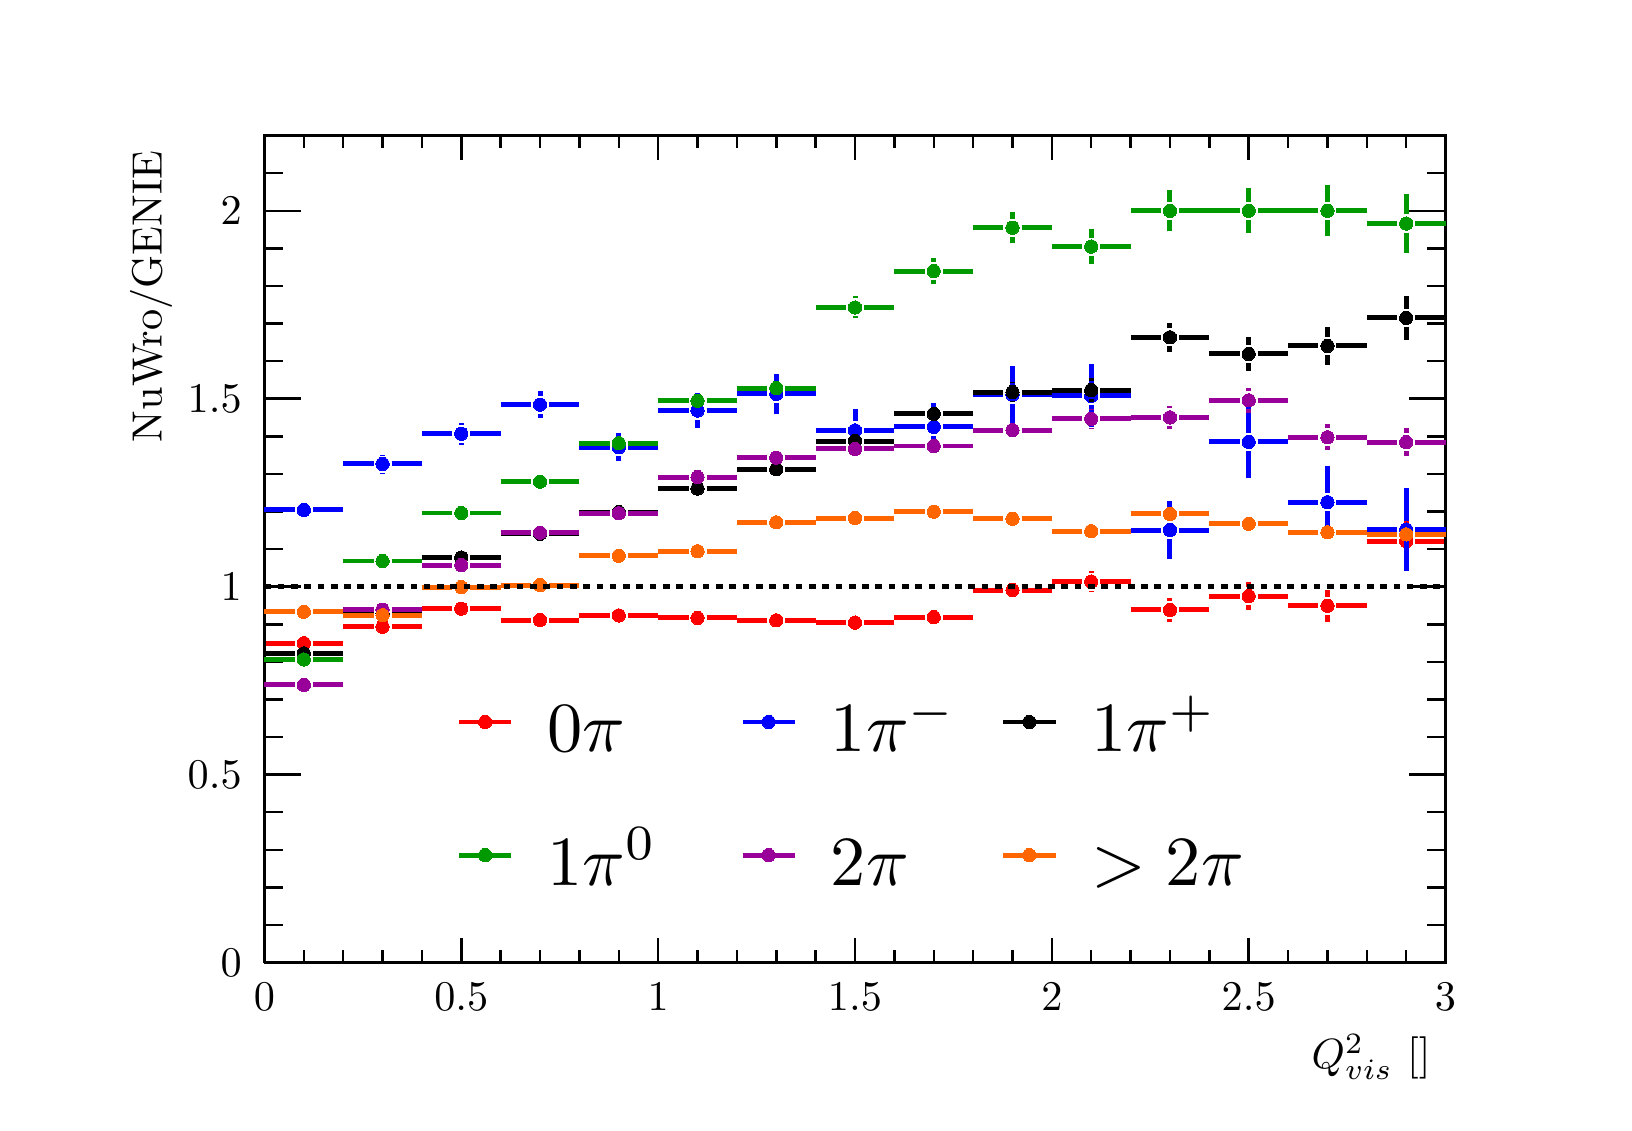
\begin{tikzpicture}
\pgfdeclareplotmark{cross} {
\pgfpathmoveto{\pgfpoint{-0.3\pgfplotmarksize}{\pgfplotmarksize}}
\pgfpathlineto{\pgfpoint{+0.3\pgfplotmarksize}{\pgfplotmarksize}}
\pgfpathlineto{\pgfpoint{+0.3\pgfplotmarksize}{0.3\pgfplotmarksize}}
\pgfpathlineto{\pgfpoint{+1\pgfplotmarksize}{0.3\pgfplotmarksize}}
\pgfpathlineto{\pgfpoint{+1\pgfplotmarksize}{-0.3\pgfplotmarksize}}
\pgfpathlineto{\pgfpoint{+0.3\pgfplotmarksize}{-0.3\pgfplotmarksize}}
\pgfpathlineto{\pgfpoint{+0.3\pgfplotmarksize}{-1.\pgfplotmarksize}}
\pgfpathlineto{\pgfpoint{-0.3\pgfplotmarksize}{-1.\pgfplotmarksize}}
\pgfpathlineto{\pgfpoint{-0.3\pgfplotmarksize}{-0.3\pgfplotmarksize}}
\pgfpathlineto{\pgfpoint{-1.\pgfplotmarksize}{-0.3\pgfplotmarksize}}
\pgfpathlineto{\pgfpoint{-1.\pgfplotmarksize}{0.3\pgfplotmarksize}}
\pgfpathlineto{\pgfpoint{-0.3\pgfplotmarksize}{0.3\pgfplotmarksize}}
\pgfpathclose
\pgfusepathqstroke
}
\pgfdeclareplotmark{cross*} {
\pgfpathmoveto{\pgfpoint{-0.3\pgfplotmarksize}{\pgfplotmarksize}}
\pgfpathlineto{\pgfpoint{+0.3\pgfplotmarksize}{\pgfplotmarksize}}
\pgfpathlineto{\pgfpoint{+0.3\pgfplotmarksize}{0.3\pgfplotmarksize}}
\pgfpathlineto{\pgfpoint{+1\pgfplotmarksize}{0.3\pgfplotmarksize}}
\pgfpathlineto{\pgfpoint{+1\pgfplotmarksize}{-0.3\pgfplotmarksize}}
\pgfpathlineto{\pgfpoint{+0.3\pgfplotmarksize}{-0.3\pgfplotmarksize}}
\pgfpathlineto{\pgfpoint{+0.3\pgfplotmarksize}{-1.\pgfplotmarksize}}
\pgfpathlineto{\pgfpoint{-0.3\pgfplotmarksize}{-1.\pgfplotmarksize}}
\pgfpathlineto{\pgfpoint{-0.3\pgfplotmarksize}{-0.3\pgfplotmarksize}}
\pgfpathlineto{\pgfpoint{-1.\pgfplotmarksize}{-0.3\pgfplotmarksize}}
\pgfpathlineto{\pgfpoint{-1.\pgfplotmarksize}{0.3\pgfplotmarksize}}
\pgfpathlineto{\pgfpoint{-0.3\pgfplotmarksize}{0.3\pgfplotmarksize}}
\pgfpathclose
\pgfusepathqfillstroke
}
\pgfdeclareplotmark{newstar} {
\pgfpathmoveto{\pgfqpoint{0pt}{\pgfplotmarksize}}
\pgfpathlineto{\pgfqpointpolar{44}{0.5\pgfplotmarksize}}
\pgfpathlineto{\pgfqpointpolar{18}{\pgfplotmarksize}}
\pgfpathlineto{\pgfqpointpolar{-20}{0.5\pgfplotmarksize}}
\pgfpathlineto{\pgfqpointpolar{-54}{\pgfplotmarksize}}
\pgfpathlineto{\pgfqpointpolar{-90}{0.5\pgfplotmarksize}}
\pgfpathlineto{\pgfqpointpolar{234}{\pgfplotmarksize}}
\pgfpathlineto{\pgfqpointpolar{198}{0.5\pgfplotmarksize}}
\pgfpathlineto{\pgfqpointpolar{162}{\pgfplotmarksize}}
\pgfpathlineto{\pgfqpointpolar{134}{0.5\pgfplotmarksize}}
\pgfpathclose
\pgfusepathqstroke
}
\pgfdeclareplotmark{newstar*} {
\pgfpathmoveto{\pgfqpoint{0pt}{\pgfplotmarksize}}
\pgfpathlineto{\pgfqpointpolar{44}{0.5\pgfplotmarksize}}
\pgfpathlineto{\pgfqpointpolar{18}{\pgfplotmarksize}}
\pgfpathlineto{\pgfqpointpolar{-20}{0.5\pgfplotmarksize}}
\pgfpathlineto{\pgfqpointpolar{-54}{\pgfplotmarksize}}
\pgfpathlineto{\pgfqpointpolar{-90}{0.5\pgfplotmarksize}}
\pgfpathlineto{\pgfqpointpolar{234}{\pgfplotmarksize}}
\pgfpathlineto{\pgfqpointpolar{198}{0.5\pgfplotmarksize}}
\pgfpathlineto{\pgfqpointpolar{162}{\pgfplotmarksize}}
\pgfpathlineto{\pgfqpointpolar{134}{0.5\pgfplotmarksize}}
\pgfpathclose
\pgfusepathqfillstroke
}
\definecolor{c}{rgb}{1,1,1};
\draw [color=c, fill=c] (0,0) rectangle (20,13.639);
\draw [color=c, fill=c] (3,1.77307) rectangle (18,12.2751);
\definecolor{c}{rgb}{0,0,0};
\draw [c,line width=0.9] (3,1.77307) -- (3,12.2751) -- (18,12.2751) -- (18,1.77307) -- (3,1.77307);
\definecolor{c}{rgb}{1,1,1};
\draw [color=c, fill=c] (3,1.77307) rectangle (18,12.2751);
\definecolor{c}{rgb}{0,0,0};
\draw [c,line width=0.9] (3,1.77307) -- (3,12.2751) -- (18,12.2751) -- (18,1.77307) -- (3,1.77307);
\definecolor{c}{rgb}{1,0,0};
\draw [c,line width=1.8] (3,5.82886) -- (3.38539,5.82886);
\draw [c,line width=1.8] (3.61461,5.82886) -- (4,5.82886);
\foreach \P in {(3.5,5.82886)}{\draw[mark options={color=c,fill=c},mark size=2.402402pt, line width=0.000000pt, mark=*] plot coordinates {\P};}
\draw [c,line width=1.8] (4,6.03849) -- (4.38539,6.03849);
\draw [c,line width=1.8] (4.61461,6.03849) -- (5,6.03849);
\foreach \P in {(4.5,6.03849)}{\draw[mark options={color=c,fill=c},mark size=2.402402pt, line width=0.000000pt, mark=*] plot coordinates {\P};}
\draw [c,line width=1.8] (5,6.26711) -- (5.38539,6.26711);
\draw [c,line width=1.8] (5.61461,6.26711) -- (6,6.26711);
\foreach \P in {(5.5,6.26711)}{\draw[mark options={color=c,fill=c},mark size=2.402402pt, line width=0.000000pt, mark=*] plot coordinates {\P};}
\draw [c,line width=1.8] (6,6.12288) -- (6.38539,6.12288);
\draw [c,line width=1.8] (6.61461,6.12288) -- (7,6.12288);
\foreach \P in {(6.5,6.12288)}{\draw[mark options={color=c,fill=c},mark size=2.402402pt, line width=0.000000pt, mark=*] plot coordinates {\P};}
\draw [c,line width=1.8] (7,6.18166) -- (7.38539,6.18166);
\draw [c,line width=1.8] (7.61461,6.18166) -- (8,6.18166);
\foreach \P in {(7.5,6.18166)}{\draw[mark options={color=c,fill=c},mark size=2.402402pt, line width=0.000000pt, mark=*] plot coordinates {\P};}
\draw [c,line width=1.8] (8,6.14986) -- (8.38539,6.14986);
\draw [c,line width=1.8] (8.61461,6.14986) -- (9,6.14986);
\foreach \P in {(8.5,6.14986)}{\draw[mark options={color=c,fill=c},mark size=2.402402pt, line width=0.000000pt, mark=*] plot coordinates {\P};}
\draw [c,line width=1.8] (9,6.11908) -- (9.38539,6.11908);
\draw [c,line width=1.8] (9.61461,6.11908) -- (10,6.11908);
\foreach \P in {(9.5,6.11908)}{\draw[mark options={color=c,fill=c},mark size=2.402402pt, line width=0.000000pt, mark=*] plot coordinates {\P};}
\draw [c,line width=1.8] (10,6.08987) -- (10.3854,6.08987);
\draw [c,line width=1.8] (10.6146,6.08987) -- (11,6.08987);
\foreach \P in {(10.5,6.08987)}{\draw[mark options={color=c,fill=c},mark size=2.402402pt, line width=0.000000pt, mark=*] plot coordinates {\P};}
\draw [c,line width=1.8] (11,6.16035) -- (11.3854,6.16035);
\draw [c,line width=1.8] (11.6146,6.16035) -- (12,6.16035);
\foreach \P in {(11.5,6.16035)}{\draw[mark options={color=c,fill=c},mark size=2.402402pt, line width=0.000000pt, mark=*] plot coordinates {\P};}
\draw [c,line width=1.8] (12,6.50381) -- (12.3854,6.50381);
\draw [c,line width=1.8] (12.6146,6.50381) -- (13,6.50381);
\foreach \P in {(12.5,6.50381)}{\draw[mark options={color=c,fill=c},mark size=2.402402pt, line width=0.000000pt, mark=*] plot coordinates {\P};}
\draw [c,line width=1.8] (13.5,6.47964) -- (13.5,6.49613);
\draw [c,line width=1.8] (13.5,6.72535) -- (13.5,6.74184);
\draw [c,line width=1.8] (13,6.61074) -- (13.3854,6.61074);
\draw [c,line width=1.8] (13.6146,6.61074) -- (14,6.61074);
\foreach \P in {(13.5,6.61074)}{\draw[mark options={color=c,fill=c},mark size=2.402402pt, line width=0.000000pt, mark=*] plot coordinates {\P};}
\draw [c,line width=1.8] (14.5,6.10391) -- (14.5,6.13613);
\draw [c,line width=1.8] (14.5,6.36536) -- (14.5,6.39759);
\draw [c,line width=1.8] (14,6.25075) -- (14.3854,6.25075);
\draw [c,line width=1.8] (14.6146,6.25075) -- (15,6.25075);
\foreach \P in {(14.5,6.25075)}{\draw[mark options={color=c,fill=c},mark size=2.402402pt, line width=0.000000pt, mark=*] plot coordinates {\P};}
\draw [c,line width=1.8] (15.5,6.25269) -- (15.5,6.31279);
\draw [c,line width=1.8] (15.5,6.54202) -- (15.5,6.60213);
\draw [c,line width=1.8] (15,6.42741) -- (15.3854,6.42741);
\draw [c,line width=1.8] (15.6146,6.42741) -- (16,6.42741);
\foreach \P in {(15.5,6.42741)}{\draw[mark options={color=c,fill=c},mark size=2.402402pt, line width=0.000000pt, mark=*] plot coordinates {\P};}
\draw [c,line width=1.8] (16.5,6.10359) -- (16.5,6.18975);
\draw [c,line width=1.8] (16.5,6.41898) -- (16.5,6.50514);
\draw [c,line width=1.8] (16,6.30436) -- (16.3854,6.30436);
\draw [c,line width=1.8] (16.6146,6.30436) -- (17,6.30436);
\foreach \P in {(16.5,6.30436)}{\draw[mark options={color=c,fill=c},mark size=2.402402pt, line width=0.000000pt, mark=*] plot coordinates {\P};}
\draw [c,line width=1.8] (17.5,6.87193) -- (17.5,7.01171);
\draw [c,line width=1.8] (17.5,7.24094) -- (17.5,7.38072);
\draw [c,line width=1.8] (17,7.12632) -- (17.3854,7.12632);
\draw [c,line width=1.8] (17.6146,7.12632) -- (18,7.12632);
\foreach \P in {(17.5,7.12632)}{\draw[mark options={color=c,fill=c},mark size=2.402402pt, line width=0.000000pt, mark=*] plot coordinates {\P};}
\definecolor{c}{rgb}{0,0,0};
\draw [c,line width=0.9] (3,1.77307) -- (18,1.77307);
\draw [c,line width=0.9] (3,2.07994) -- (3,1.77307);
\draw [c,line width=0.9] (3.5,1.9265) -- (3.5,1.77307);
\draw [c,line width=0.9] (4,1.9265) -- (4,1.77307);
\draw [c,line width=0.9] (4.5,1.9265) -- (4.5,1.77307);
\draw [c,line width=0.9] (5,1.9265) -- (5,1.77307);
\draw [c,line width=0.9] (5.5,2.07994) -- (5.5,1.77307);
\draw [c,line width=0.9] (6,1.9265) -- (6,1.77307);
\draw [c,line width=0.9] (6.5,1.9265) -- (6.5,1.77307);
\draw [c,line width=0.9] (7,1.9265) -- (7,1.77307);
\draw [c,line width=0.9] (7.5,1.9265) -- (7.5,1.77307);
\draw [c,line width=0.9] (8,2.07994) -- (8,1.77307);
\draw [c,line width=0.9] (8.5,1.9265) -- (8.5,1.77307);
\draw [c,line width=0.9] (9,1.9265) -- (9,1.77307);
\draw [c,line width=0.9] (9.5,1.9265) -- (9.5,1.77307);
\draw [c,line width=0.9] (10,1.9265) -- (10,1.77307);
\draw [c,line width=0.9] (10.5,2.07994) -- (10.5,1.77307);
\draw [c,line width=0.9] (11,1.9265) -- (11,1.77307);
\draw [c,line width=0.9] (11.5,1.9265) -- (11.5,1.77307);
\draw [c,line width=0.9] (12,1.9265) -- (12,1.77307);
\draw [c,line width=0.9] (12.5,1.9265) -- (12.5,1.77307);
\draw [c,line width=0.9] (13,2.07994) -- (13,1.77307);
\draw [c,line width=0.9] (13.5,1.9265) -- (13.5,1.77307);
\draw [c,line width=0.9] (14,1.9265) -- (14,1.77307);
\draw [c,line width=0.9] (14.5,1.9265) -- (14.5,1.77307);
\draw [c,line width=0.9] (15,1.9265) -- (15,1.77307);
\draw [c,line width=0.9] (15.5,2.07994) -- (15.5,1.77307);
\draw [c,line width=0.9] (16,1.9265) -- (16,1.77307);
\draw [c,line width=0.9] (16.5,1.9265) -- (16.5,1.77307);
\draw [c,line width=0.9] (17,1.9265) -- (17,1.77307);
\draw [c,line width=0.9] (17.5,1.9265) -- (17.5,1.77307);
\draw [c,line width=0.9] (18,2.07994) -- (18,1.77307);
\draw [c,line width=0.9] (18,2.07994) -- (18,1.77307);
\draw [anchor=base] (3,1.15931) node[scale=1.52731, color=c, rotate=0]{0};
\draw [anchor=base] (5.5,1.15931) node[scale=1.52731, color=c, rotate=0]{0.5};
\draw [anchor=base] (8,1.15931) node[scale=1.52731, color=c, rotate=0]{1};
\draw [anchor=base] (10.5,1.15931) node[scale=1.52731, color=c, rotate=0]{1.5};
\draw [anchor=base] (13,1.15931) node[scale=1.52731, color=c, rotate=0]{2};
\draw [anchor=base] (15.5,1.15931) node[scale=1.52731, color=c, rotate=0]{2.5};
\draw [anchor=base] (18,1.15931) node[scale=1.52731, color=c, rotate=0]{3};
\draw [anchor= east] (18,0.572837) node[scale=1.52731, color=c, rotate=0]{$Q^{2}_{\text{vis}}$ [\si{\giga\electronvolt\squared}] };
\draw [c,line width=0.9] (3,12.2751) -- (18,12.2751);
\draw [c,line width=0.9] (3,11.9682) -- (3,12.2751);
\draw [c,line width=0.9] (3.5,12.1216) -- (3.5,12.2751);
\draw [c,line width=0.9] (4,12.1216) -- (4,12.2751);
\draw [c,line width=0.9] (4.5,12.1216) -- (4.5,12.2751);
\draw [c,line width=0.9] (5,12.1216) -- (5,12.2751);
\draw [c,line width=0.9] (5.5,11.9682) -- (5.5,12.2751);
\draw [c,line width=0.9] (6,12.1216) -- (6,12.2751);
\draw [c,line width=0.9] (6.5,12.1216) -- (6.5,12.2751);
\draw [c,line width=0.9] (7,12.1216) -- (7,12.2751);
\draw [c,line width=0.9] (7.5,12.1216) -- (7.5,12.2751);
\draw [c,line width=0.9] (8,11.9682) -- (8,12.2751);
\draw [c,line width=0.9] (8.5,12.1216) -- (8.5,12.2751);
\draw [c,line width=0.9] (9,12.1216) -- (9,12.2751);
\draw [c,line width=0.9] (9.5,12.1216) -- (9.5,12.2751);
\draw [c,line width=0.9] (10,12.1216) -- (10,12.2751);
\draw [c,line width=0.9] (10.5,11.9682) -- (10.5,12.2751);
\draw [c,line width=0.9] (11,12.1216) -- (11,12.2751);
\draw [c,line width=0.9] (11.5,12.1216) -- (11.5,12.2751);
\draw [c,line width=0.9] (12,12.1216) -- (12,12.2751);
\draw [c,line width=0.9] (12.5,12.1216) -- (12.5,12.2751);
\draw [c,line width=0.9] (13,11.9682) -- (13,12.2751);
\draw [c,line width=0.9] (13.5,12.1216) -- (13.5,12.2751);
\draw [c,line width=0.9] (14,12.1216) -- (14,12.2751);
\draw [c,line width=0.9] (14.5,12.1216) -- (14.5,12.2751);
\draw [c,line width=0.9] (15,12.1216) -- (15,12.2751);
\draw [c,line width=0.9] (15.5,11.9682) -- (15.5,12.2751);
\draw [c,line width=0.9] (16,12.1216) -- (16,12.2751);
\draw [c,line width=0.9] (16.5,12.1216) -- (16.5,12.2751);
\draw [c,line width=0.9] (17,12.1216) -- (17,12.2751);
\draw [c,line width=0.9] (17.5,12.1216) -- (17.5,12.2751);
\draw [c,line width=0.9] (18,11.9682) -- (18,12.2751);
\draw [c,line width=0.9] (18,11.9682) -- (18,12.2751);
\draw [c,line width=0.9] (3,1.77307) -- (3,12.2751);
\draw [c,line width=0.9] (3.462,1.77307) -- (3,1.77307);
\draw [c,line width=0.9] (3.231,2.25043) -- (3,2.25043);
\draw [c,line width=0.9] (3.231,2.72779) -- (3,2.72779);
\draw [c,line width=0.9] (3.231,3.20516) -- (3,3.20516);
\draw [c,line width=0.9] (3.231,3.68252) -- (3,3.68252);
\draw [c,line width=0.9] (3.462,4.15989) -- (3,4.15989);
\draw [c,line width=0.9] (3.231,4.63725) -- (3,4.63725);
\draw [c,line width=0.9] (3.231,5.11461) -- (3,5.11461);
\draw [c,line width=0.9] (3.231,5.59198) -- (3,5.59198);
\draw [c,line width=0.9] (3.231,6.06934) -- (3,6.06934);
\draw [c,line width=0.9] (3.462,6.5467) -- (3,6.5467);
\draw [c,line width=0.9] (3.231,7.02407) -- (3,7.02407);
\draw [c,line width=0.9] (3.231,7.50143) -- (3,7.50143);
\draw [c,line width=0.9] (3.231,7.9788) -- (3,7.9788);
\draw [c,line width=0.9] (3.231,8.45616) -- (3,8.45616);
\draw [c,line width=0.9] (3.462,8.93352) -- (3,8.93352);
\draw [c,line width=0.9] (3.231,9.41089) -- (3,9.41089);
\draw [c,line width=0.9] (3.231,9.88825) -- (3,9.88825);
\draw [c,line width=0.9] (3.231,10.3656) -- (3,10.3656);
\draw [c,line width=0.9] (3.231,10.843) -- (3,10.843);
\draw [c,line width=0.9] (3.462,11.3203) -- (3,11.3203);
\draw [c,line width=0.9] (3.462,11.3203) -- (3,11.3203);
\draw [c,line width=0.9] (3.231,11.7977) -- (3,11.7977);
\draw [c,line width=0.9] (3.231,12.2751) -- (3,12.2751);
\draw [anchor= east] (2.9,1.77307) node[scale=1.52731, color=c, rotate=0]{0};
\draw [anchor= east] (2.9,4.15989) node[scale=1.52731, color=c, rotate=0]{0.5};
\draw [anchor= east] (2.9,6.5467) node[scale=1.52731, color=c, rotate=0]{1};
\draw [anchor= east] (2.9,8.93352) node[scale=1.52731, color=c, rotate=0]{1.5};
\draw [anchor= east] (2.9,11.3203) node[scale=1.52731, color=c, rotate=0]{2};
\draw [anchor= east] (1.56,12.2751) node[scale=1.52731, color=c, rotate=90]{ NuWro/GENIE};
\draw [c,line width=0.9] (18,1.77307) -- (18,12.2751);
\draw [c,line width=0.9] (17.538,1.77307) -- (18,1.77307);
\draw [c,line width=0.9] (17.769,2.25043) -- (18,2.25043);
\draw [c,line width=0.9] (17.769,2.72779) -- (18,2.72779);
\draw [c,line width=0.9] (17.769,3.20516) -- (18,3.20516);
\draw [c,line width=0.9] (17.769,3.68252) -- (18,3.68252);
\draw [c,line width=0.9] (17.538,4.15989) -- (18,4.15989);
\draw [c,line width=0.9] (17.769,4.63725) -- (18,4.63725);
\draw [c,line width=0.9] (17.769,5.11461) -- (18,5.11461);
\draw [c,line width=0.9] (17.769,5.59198) -- (18,5.59198);
\draw [c,line width=0.9] (17.769,6.06934) -- (18,6.06934);
\draw [c,line width=0.9] (17.538,6.5467) -- (18,6.5467);
\draw [c,line width=0.9] (17.769,7.02407) -- (18,7.02407);
\draw [c,line width=0.9] (17.769,7.50143) -- (18,7.50143);
\draw [c,line width=0.9] (17.769,7.9788) -- (18,7.9788);
\draw [c,line width=0.9] (17.769,8.45616) -- (18,8.45616);
\draw [c,line width=0.9] (17.538,8.93352) -- (18,8.93352);
\draw [c,line width=0.9] (17.769,9.41089) -- (18,9.41089);
\draw [c,line width=0.9] (17.769,9.88825) -- (18,9.88825);
\draw [c,line width=0.9] (17.769,10.3656) -- (18,10.3656);
\draw [c,line width=0.9] (17.769,10.843) -- (18,10.843);
\draw [c,line width=0.9] (17.538,11.3203) -- (18,11.3203);
\draw [c,line width=0.9] (17.538,11.3203) -- (18,11.3203);
\draw [c,line width=0.9] (17.769,11.7977) -- (18,11.7977);
\draw [c,line width=0.9] (17.769,12.2751) -- (18,12.2751);
\definecolor{c}{rgb}{0,0,1};
\draw [c,line width=1.8] (3,7.52061) -- (3.38539,7.52061);
\draw [c,line width=1.8] (3.61461,7.52061) -- (4,7.52061);
\foreach \P in {(3.5,7.52061)}{\draw[mark options={color=c,fill=c},mark size=2.402402pt, line width=0.000000pt, mark=*] plot coordinates {\P};}
\draw [c,line width=1.8] (4.5,7.98956) -- (4.5,7.99026);
\draw [c,line width=1.8] (4.5,8.21949) -- (4.5,8.22019);
\draw [c,line width=1.8] (4,8.10488) -- (4.38539,8.10488);
\draw [c,line width=1.8] (4.61461,8.10488) -- (5,8.10488);
\foreach \P in {(4.5,8.10488)}{\draw[mark options={color=c,fill=c},mark size=2.402402pt, line width=0.000000pt, mark=*] plot coordinates {\P};}
\draw [c,line width=1.8] (5.5,8.3504) -- (5.5,8.37484);
\draw [c,line width=1.8] (5.5,8.60406) -- (5.5,8.6285);
\draw [c,line width=1.8] (5,8.48945) -- (5.38539,8.48945);
\draw [c,line width=1.8] (5.61461,8.48945) -- (6,8.48945);
\foreach \P in {(5.5,8.48945)}{\draw[mark options={color=c,fill=c},mark size=2.402402pt, line width=0.000000pt, mark=*] plot coordinates {\P};}
\draw [c,line width=1.8] (6.5,8.68828) -- (6.5,8.74365);
\draw [c,line width=1.8] (6.5,8.97288) -- (6.5,9.02825);
\draw [c,line width=1.8] (6,8.85826) -- (6.38539,8.85826);
\draw [c,line width=1.8] (6.61461,8.85826) -- (7,8.85826);
\foreach \P in {(6.5,8.85826)}{\draw[mark options={color=c,fill=c},mark size=2.402402pt, line width=0.000000pt, mark=*] plot coordinates {\P};}
\draw [c,line width=1.8] (7.5,8.13763) -- (7.5,8.20169);
\draw [c,line width=1.8] (7.5,8.43091) -- (7.5,8.49497);
\draw [c,line width=1.8] (7,8.3163) -- (7.38539,8.3163);
\draw [c,line width=1.8] (7.61461,8.3163) -- (8,8.3163);
\foreach \P in {(7.5,8.3163)}{\draw[mark options={color=c,fill=c},mark size=2.402402pt, line width=0.000000pt, mark=*] plot coordinates {\P};}
\draw [c,line width=1.8] (8.5,8.56533) -- (8.5,8.66955);
\draw [c,line width=1.8] (8.5,8.89877) -- (8.5,9.00299);
\draw [c,line width=1.8] (8,8.78416) -- (8.38539,8.78416);
\draw [c,line width=1.8] (8.61461,8.78416) -- (9,8.78416);
\foreach \P in {(8.5,8.78416)}{\draw[mark options={color=c,fill=c},mark size=2.402402pt, line width=0.000000pt, mark=*] plot coordinates {\P};}
\draw [c,line width=1.8] (9.5,8.74004) -- (9.5,8.87982);
\draw [c,line width=1.8] (9.5,9.10905) -- (9.5,9.24883);
\draw [c,line width=1.8] (9,8.99443) -- (9.38539,8.99443);
\draw [c,line width=1.8] (9.61461,8.99443) -- (10,8.99443);
\foreach \P in {(9.5,8.99443)}{\draw[mark options={color=c,fill=c},mark size=2.402402pt, line width=0.000000pt, mark=*] plot coordinates {\P};}
\draw [c,line width=1.8] (10.5,8.25734) -- (10.5,8.41721);
\draw [c,line width=1.8] (10.5,8.64643) -- (10.5,8.8063);
\draw [c,line width=1.8] (10,8.53182) -- (10.3854,8.53182);
\draw [c,line width=1.8] (10.6146,8.53182) -- (11,8.53182);
\foreach \P in {(10.5,8.53182)}{\draw[mark options={color=c,fill=c},mark size=2.402402pt, line width=0.000000pt, mark=*] plot coordinates {\P};}
\draw [c,line width=1.8] (11.5,8.2699) -- (11.5,8.46171);
\draw [c,line width=1.8] (11.5,8.69094) -- (11.5,8.88275);
\draw [c,line width=1.8] (11,8.57632) -- (11.3854,8.57632);
\draw [c,line width=1.8] (11.6146,8.57632) -- (12,8.57632);
\foreach \P in {(11.5,8.57632)}{\draw[mark options={color=c,fill=c},mark size=2.402402pt, line width=0.000000pt, mark=*] plot coordinates {\P};}
\draw [c,line width=1.8] (12.5,8.61854) -- (12.5,8.87227);
\draw [c,line width=1.8] (12.5,9.1015) -- (12.5,9.35523);
\draw [c,line width=1.8] (12,8.98688) -- (12.3854,8.98688);
\draw [c,line width=1.8] (12.6146,8.98688) -- (13,8.98688);
\foreach \P in {(12.5,8.98688)}{\draw[mark options={color=c,fill=c},mark size=2.402402pt, line width=0.000000pt, mark=*] plot coordinates {\P};}
\draw [c,line width=1.8] (13.5,8.56917) -- (13.5,8.85412);
\draw [c,line width=1.8] (13.5,9.08334) -- (13.5,9.36829);
\draw [c,line width=1.8] (13,8.96873) -- (13.3854,8.96873);
\draw [c,line width=1.8] (13.6146,8.96873) -- (14,8.96873);
\foreach \P in {(13.5,8.96873)}{\draw[mark options={color=c,fill=c},mark size=2.402402pt, line width=0.000000pt, mark=*] plot coordinates {\P};}
\draw [c,line width=1.8] (14.5,6.89727) -- (14.5,7.15055);
\draw [c,line width=1.8] (14.5,7.37978) -- (14.5,7.63306);
\draw [c,line width=1.8] (14,7.26516) -- (14.3854,7.26516);
\draw [c,line width=1.8] (14.6146,7.26516) -- (15,7.26516);
\foreach \P in {(14.5,7.26516)}{\draw[mark options={color=c,fill=c},mark size=2.402402pt, line width=0.000000pt, mark=*] plot coordinates {\P};}
\draw [c,line width=1.8] (15.5,7.92354) -- (15.5,8.27087);
\draw [c,line width=1.8] (15.5,8.5001) -- (15.5,8.84743);
\draw [c,line width=1.8] (15,8.38549) -- (15.3854,8.38549);
\draw [c,line width=1.8] (15.6146,8.38549) -- (16,8.38549);
\foreach \P in {(15.5,8.38549)}{\draw[mark options={color=c,fill=c},mark size=2.402402pt, line width=0.000000pt, mark=*] plot coordinates {\P};}
\draw [c,line width=1.8] (16.5,7.16342) -- (16.5,7.50513);
\draw [c,line width=1.8] (16.5,7.73436) -- (16.5,8.07607);
\draw [c,line width=1.8] (16,7.61974) -- (16.3854,7.61974);
\draw [c,line width=1.8] (16.6146,7.61974) -- (17,7.61974);
\foreach \P in {(16.5,7.61974)}{\draw[mark options={color=c,fill=c},mark size=2.402402pt, line width=0.000000pt, mark=*] plot coordinates {\P};}
\draw [c,line width=1.8] (17.5,6.74312) -- (17.5,7.15648);
\draw [c,line width=1.8] (17.5,7.38571) -- (17.5,7.79908);
\draw [c,line width=1.8] (17,7.2711) -- (17.3854,7.2711);
\draw [c,line width=1.8] (17.6146,7.2711) -- (18,7.2711);
\foreach \P in {(17.5,7.2711)}{\draw[mark options={color=c,fill=c},mark size=2.402402pt, line width=0.000000pt, mark=*] plot coordinates {\P};}
\definecolor{c}{rgb}{0,0,0};
\draw [c,line width=1.8] (3,5.69971) -- (3.38539,5.69971);
\draw [c,line width=1.8] (3.61461,5.69971) -- (4,5.69971);
\foreach \P in {(3.5,5.69971)}{\draw[mark options={color=c,fill=c},mark size=2.402402pt, line width=0.000000pt, mark=*] plot coordinates {\P};}
\draw [c,line width=1.8] (4,6.20869) -- (4.38539,6.20869);
\draw [c,line width=1.8] (4.61461,6.20869) -- (5,6.20869);
\foreach \P in {(4.5,6.20869)}{\draw[mark options={color=c,fill=c},mark size=2.402402pt, line width=0.000000pt, mark=*] plot coordinates {\P};}
\draw [c,line width=1.8] (5,6.91728) -- (5.38539,6.91728);
\draw [c,line width=1.8] (5.61461,6.91728) -- (6,6.91728);
\foreach \P in {(5.5,6.91728)}{\draw[mark options={color=c,fill=c},mark size=2.402402pt, line width=0.000000pt, mark=*] plot coordinates {\P};}
\draw [c,line width=1.8] (6,7.21845) -- (6.38539,7.21845);
\draw [c,line width=1.8] (6.61461,7.21845) -- (7,7.21845);
\foreach \P in {(6.5,7.21845)}{\draw[mark options={color=c,fill=c},mark size=2.402402pt, line width=0.000000pt, mark=*] plot coordinates {\P};}
\draw [c,line width=1.8] (7,7.49374) -- (7.38539,7.49374);
\draw [c,line width=1.8] (7.61461,7.49374) -- (8,7.49374);
\foreach \P in {(7.5,7.49374)}{\draw[mark options={color=c,fill=c},mark size=2.402402pt, line width=0.000000pt, mark=*] plot coordinates {\P};}
\draw [c,line width=1.8] (8,7.79179) -- (8.38539,7.79179);
\draw [c,line width=1.8] (8.61461,7.79179) -- (9,7.79179);
\foreach \P in {(8.5,7.79179)}{\draw[mark options={color=c,fill=c},mark size=2.402402pt, line width=0.000000pt, mark=*] plot coordinates {\P};}
\draw [c,line width=1.8] (9,8.03695) -- (9.38539,8.03695);
\draw [c,line width=1.8] (9.61461,8.03695) -- (10,8.03695);
\foreach \P in {(9.5,8.03695)}{\draw[mark options={color=c,fill=c},mark size=2.402402pt, line width=0.000000pt, mark=*] plot coordinates {\P};}
\draw [c,line width=1.8] (10,8.3953) -- (10.3854,8.3953);
\draw [c,line width=1.8] (10.6146,8.3953) -- (11,8.3953);
\foreach \P in {(10.5,8.3953)}{\draw[mark options={color=c,fill=c},mark size=2.402402pt, line width=0.000000pt, mark=*] plot coordinates {\P};}
\draw [c,line width=1.8] (11,8.74131) -- (11.3854,8.74131);
\draw [c,line width=1.8] (11.6146,8.74131) -- (12,8.74131);
\foreach \P in {(11.5,8.74131)}{\draw[mark options={color=c,fill=c},mark size=2.402402pt, line width=0.000000pt, mark=*] plot coordinates {\P};}
\draw [c,line width=1.8] (12.5,8.88845) -- (12.5,8.90289);
\draw [c,line width=1.8] (12.5,9.13212) -- (12.5,9.14656);
\draw [c,line width=1.8] (12,9.01751) -- (12.3854,9.01751);
\draw [c,line width=1.8] (12.6146,9.01751) -- (13,9.01751);
\foreach \P in {(12.5,9.01751)}{\draw[mark options={color=c,fill=c},mark size=2.402402pt, line width=0.000000pt, mark=*] plot coordinates {\P};}
\draw [c,line width=1.8] (13.5,8.89535) -- (13.5,8.92859);
\draw [c,line width=1.8] (13.5,9.15782) -- (13.5,9.19107);
\draw [c,line width=1.8] (13,9.04321) -- (13.3854,9.04321);
\draw [c,line width=1.8] (13.6146,9.04321) -- (14,9.04321);
\foreach \P in {(13.5,9.04321)}{\draw[mark options={color=c,fill=c},mark size=2.402402pt, line width=0.000000pt, mark=*] plot coordinates {\P};}
\draw [c,line width=1.8] (14.5,9.52667) -- (14.5,9.59931);
\draw [c,line width=1.8] (14.5,9.82853) -- (14.5,9.90117);
\draw [c,line width=1.8] (14,9.71392) -- (14.3854,9.71392);
\draw [c,line width=1.8] (14.6146,9.71392) -- (15,9.71392);
\foreach \P in {(14.5,9.71392)}{\draw[mark options={color=c,fill=c},mark size=2.402402pt, line width=0.000000pt, mark=*] plot coordinates {\P};}
\draw [c,line width=1.8] (15.5,9.29097) -- (15.5,9.38736);
\draw [c,line width=1.8] (15.5,9.61659) -- (15.5,9.71298);
\draw [c,line width=1.8] (15,9.50198) -- (15.3854,9.50198);
\draw [c,line width=1.8] (15.6146,9.50198) -- (16,9.50198);
\foreach \P in {(15.5,9.50198)}{\draw[mark options={color=c,fill=c},mark size=2.402402pt, line width=0.000000pt, mark=*] plot coordinates {\P};}
\draw [c,line width=1.8] (16.5,9.36249) -- (16.5,9.48996);
\draw [c,line width=1.8] (16.5,9.71919) -- (16.5,9.84666);
\draw [c,line width=1.8] (16,9.60458) -- (16.3854,9.60458);
\draw [c,line width=1.8] (16.6146,9.60458) -- (17,9.60458);
\foreach \P in {(16.5,9.60458)}{\draw[mark options={color=c,fill=c},mark size=2.402402pt, line width=0.000000pt, mark=*] plot coordinates {\P};}
\draw [c,line width=1.8] (17.5,9.67941) -- (17.5,9.84565);
\draw [c,line width=1.8] (17.5,10.0749) -- (17.5,10.2411);
\draw [c,line width=1.8] (17,9.96026) -- (17.3854,9.96026);
\draw [c,line width=1.8] (17.6146,9.96026) -- (18,9.96026);
\foreach \P in {(17.5,9.96026)}{\draw[mark options={color=c,fill=c},mark size=2.402402pt, line width=0.000000pt, mark=*] plot coordinates {\P};}
\definecolor{c}{rgb}{0,0.6,0};
\draw [c,line width=1.8] (3,5.62264) -- (3.38539,5.62264);
\draw [c,line width=1.8] (3.61461,5.62264) -- (4,5.62264);
\foreach \P in {(3.5,5.62264)}{\draw[mark options={color=c,fill=c},mark size=2.402402pt, line width=0.000000pt, mark=*] plot coordinates {\P};}
\draw [c,line width=1.8] (4,6.87259) -- (4.38539,6.87259);
\draw [c,line width=1.8] (4.61461,6.87259) -- (5,6.87259);
\foreach \P in {(4.5,6.87259)}{\draw[mark options={color=c,fill=c},mark size=2.402402pt, line width=0.000000pt, mark=*] plot coordinates {\P};}
\draw [c,line width=1.8] (5,7.48218) -- (5.38539,7.48218);
\draw [c,line width=1.8] (5.61461,7.48218) -- (6,7.48218);
\foreach \P in {(5.5,7.48218)}{\draw[mark options={color=c,fill=c},mark size=2.402402pt, line width=0.000000pt, mark=*] plot coordinates {\P};}
\draw [c,line width=1.8] (6,7.87976) -- (6.38539,7.87976);
\draw [c,line width=1.8] (6.61461,7.87976) -- (7,7.87976);
\foreach \P in {(6.5,7.87976)}{\draw[mark options={color=c,fill=c},mark size=2.402402pt, line width=0.000000pt, mark=*] plot coordinates {\P};}
\draw [c,line width=1.8] (7,8.36921) -- (7.38539,8.36921);
\draw [c,line width=1.8] (7.61461,8.36921) -- (8,8.36921);
\foreach \P in {(7.5,8.36921)}{\draw[mark options={color=c,fill=c},mark size=2.402402pt, line width=0.000000pt, mark=*] plot coordinates {\P};}
\draw [c,line width=1.8] (8,8.90687) -- (8.38539,8.90687);
\draw [c,line width=1.8] (8.61461,8.90687) -- (9,8.90687);
\foreach \P in {(8.5,8.90687)}{\draw[mark options={color=c,fill=c},mark size=2.402402pt, line width=0.000000pt, mark=*] plot coordinates {\P};}
\draw [c,line width=1.8] (9,9.06858) -- (9.38539,9.06858);
\draw [c,line width=1.8] (9.61461,9.06858) -- (10,9.06858);
\foreach \P in {(9.5,9.06858)}{\draw[mark options={color=c,fill=c},mark size=2.402402pt, line width=0.000000pt, mark=*] plot coordinates {\P};}
\draw [c,line width=1.8] (10.5,9.95327) -- (10.5,9.97814);
\draw [c,line width=1.8] (10.5,10.2074) -- (10.5,10.2322);
\draw [c,line width=1.8] (10,10.0928) -- (10.3854,10.0928);
\draw [c,line width=1.8] (10.6146,10.0928) -- (11,10.0928);
\foreach \P in {(10.5,10.0928)}{\draw[mark options={color=c,fill=c},mark size=2.402402pt, line width=0.000000pt, mark=*] plot coordinates {\P};}
\draw [c,line width=1.8] (11.5,10.3892) -- (11.5,10.4409);
\draw [c,line width=1.8] (11.5,10.6701) -- (11.5,10.7218);
\draw [c,line width=1.8] (11,10.5555) -- (11.3854,10.5555);
\draw [c,line width=1.8] (11.6146,10.5555) -- (12,10.5555);
\foreach \P in {(11.5,10.5555)}{\draw[mark options={color=c,fill=c},mark size=2.402402pt, line width=0.000000pt, mark=*] plot coordinates {\P};}
\draw [c,line width=1.8] (12.5,10.9078) -- (12.5,10.9911);
\draw [c,line width=1.8] (12.5,11.2203) -- (12.5,11.3035);
\draw [c,line width=1.8] (12,11.1057) -- (12.3854,11.1057);
\draw [c,line width=1.8] (12.6146,11.1057) -- (13,11.1057);
\foreach \P in {(12.5,11.1057)}{\draw[mark options={color=c,fill=c},mark size=2.402402pt, line width=0.000000pt, mark=*] plot coordinates {\P};}
\draw [c,line width=1.8] (13.5,10.6454) -- (13.5,10.7509);
\draw [c,line width=1.8] (13.5,10.9801) -- (13.5,11.0856);
\draw [c,line width=1.8] (13,10.8655) -- (13.3854,10.8655);
\draw [c,line width=1.8] (13.6146,10.8655) -- (14,10.8655);
\foreach \P in {(13.5,10.8655)}{\draw[mark options={color=c,fill=c},mark size=2.402402pt, line width=0.000000pt, mark=*] plot coordinates {\P};}
\draw [c,line width=1.8] (14.5,11.0575) -- (14.5,11.2057);
\draw [c,line width=1.8] (14.5,11.435) -- (14.5,11.5832);
\draw [c,line width=1.8] (14,11.3203) -- (14.3854,11.3203);
\draw [c,line width=1.8] (14.6146,11.3203) -- (15,11.3203);
\foreach \P in {(14.5,11.3203)}{\draw[mark options={color=c,fill=c},mark size=2.402402pt, line width=0.000000pt, mark=*] plot coordinates {\P};}
\draw [c,line width=1.8] (15.5,11.0321) -- (15.5,11.2057);
\draw [c,line width=1.8] (15.5,11.435) -- (15.5,11.6086);
\draw [c,line width=1.8] (15,11.3203) -- (15.3854,11.3203);
\draw [c,line width=1.8] (15.6146,11.3203) -- (16,11.3203);
\foreach \P in {(15.5,11.3203)}{\draw[mark options={color=c,fill=c},mark size=2.402402pt, line width=0.000000pt, mark=*] plot coordinates {\P};}
\draw [c,line width=1.8] (16.5,10.9954) -- (16.5,11.2057);
\draw [c,line width=1.8] (16.5,11.435) -- (16.5,11.6452);
\draw [c,line width=1.8] (16,11.3203) -- (16.3854,11.3203);
\draw [c,line width=1.8] (16.6146,11.3203) -- (17,11.3203);
\foreach \P in {(16.5,11.3203)}{\draw[mark options={color=c,fill=c},mark size=2.402402pt, line width=0.000000pt, mark=*] plot coordinates {\P};}
\draw [c,line width=1.8] (17.5,10.7898) -- (17.5,11.0441);
\draw [c,line width=1.8] (17.5,11.2733) -- (17.5,11.5276);
\draw [c,line width=1.8] (17,11.1587) -- (17.3854,11.1587);
\draw [c,line width=1.8] (17.6146,11.1587) -- (18,11.1587);
\foreach \P in {(17.5,11.1587)}{\draw[mark options={color=c,fill=c},mark size=2.402402pt, line width=0.000000pt, mark=*] plot coordinates {\P};}
\definecolor{c}{rgb}{0.6,0,0.6};
\draw [c,line width=1.8] (3,5.29803) -- (3.38539,5.29803);
\draw [c,line width=1.8] (3.61461,5.29803) -- (4,5.29803);
\foreach \P in {(3.5,5.29803)}{\draw[mark options={color=c,fill=c},mark size=2.402402pt, line width=0.000000pt, mark=*] plot coordinates {\P};}
\draw [c,line width=1.8] (4,6.25471) -- (4.38539,6.25471);
\draw [c,line width=1.8] (4.61461,6.25471) -- (5,6.25471);
\foreach \P in {(4.5,6.25471)}{\draw[mark options={color=c,fill=c},mark size=2.402402pt, line width=0.000000pt, mark=*] plot coordinates {\P};}
\draw [c,line width=1.8] (5,6.82104) -- (5.38539,6.82104);
\draw [c,line width=1.8] (5.61461,6.82104) -- (6,6.82104);
\foreach \P in {(5.5,6.82104)}{\draw[mark options={color=c,fill=c},mark size=2.402402pt, line width=0.000000pt, mark=*] plot coordinates {\P};}
\draw [c,line width=1.8] (6,7.23176) -- (6.38539,7.23176);
\draw [c,line width=1.8] (6.61461,7.23176) -- (7,7.23176);
\foreach \P in {(6.5,7.23176)}{\draw[mark options={color=c,fill=c},mark size=2.402402pt, line width=0.000000pt, mark=*] plot coordinates {\P};}
\draw [c,line width=1.8] (7,7.47949) -- (7.38539,7.47949);
\draw [c,line width=1.8] (7.61461,7.47949) -- (8,7.47949);
\foreach \P in {(7.5,7.47949)}{\draw[mark options={color=c,fill=c},mark size=2.402402pt, line width=0.000000pt, mark=*] plot coordinates {\P};}
\draw [c,line width=1.8] (8,7.93804) -- (8.38539,7.93804);
\draw [c,line width=1.8] (8.61461,7.93804) -- (9,7.93804);
\foreach \P in {(8.5,7.93804)}{\draw[mark options={color=c,fill=c},mark size=2.402402pt, line width=0.000000pt, mark=*] plot coordinates {\P};}
\draw [c,line width=1.8] (9,8.18466) -- (9.38539,8.18466);
\draw [c,line width=1.8] (9.61461,8.18466) -- (10,8.18466);
\foreach \P in {(9.5,8.18466)}{\draw[mark options={color=c,fill=c},mark size=2.402402pt, line width=0.000000pt, mark=*] plot coordinates {\P};}
\draw [c,line width=1.8] (10,8.29552) -- (10.3854,8.29552);
\draw [c,line width=1.8] (10.6146,8.29552) -- (11,8.29552);
\foreach \P in {(10.5,8.29552)}{\draw[mark options={color=c,fill=c},mark size=2.402402pt, line width=0.000000pt, mark=*] plot coordinates {\P};}
\draw [c,line width=1.8] (11,8.33318) -- (11.3854,8.33318);
\draw [c,line width=1.8] (11.6146,8.33318) -- (12,8.33318);
\foreach \P in {(11.5,8.33318)}{\draw[mark options={color=c,fill=c},mark size=2.402402pt, line width=0.000000pt, mark=*] plot coordinates {\P};}
\draw [c,line width=1.8] (12,8.53473) -- (12.3854,8.53473);
\draw [c,line width=1.8] (12.6146,8.53473) -- (13,8.53473);
\foreach \P in {(12.5,8.53473)}{\draw[mark options={color=c,fill=c},mark size=2.402402pt, line width=0.000000pt, mark=*] plot coordinates {\P};}
\draw [c,line width=1.8] (13.5,8.55267) -- (13.5,8.56346);
\draw [c,line width=1.8] (13.5,8.79269) -- (13.5,8.80349);
\draw [c,line width=1.8] (13,8.67808) -- (13.3854,8.67808);
\draw [c,line width=1.8] (13.6146,8.67808) -- (14,8.67808);
\foreach \P in {(13.5,8.67808)}{\draw[mark options={color=c,fill=c},mark size=2.402402pt, line width=0.000000pt, mark=*] plot coordinates {\P};}
\draw [c,line width=1.8] (14.5,8.5553) -- (14.5,8.58192);
\draw [c,line width=1.8] (14.5,8.81115) -- (14.5,8.83777);
\draw [c,line width=1.8] (14,8.69654) -- (14.3854,8.69654);
\draw [c,line width=1.8] (14.6146,8.69654) -- (15,8.69654);
\foreach \P in {(14.5,8.69654)}{\draw[mark options={color=c,fill=c},mark size=2.402402pt, line width=0.000000pt, mark=*] plot coordinates {\P};}
\draw [c,line width=1.8] (15.5,8.75403) -- (15.5,8.79878);
\draw [c,line width=1.8] (15.5,9.02801) -- (15.5,9.07276);
\draw [c,line width=1.8] (15,8.9134) -- (15.3854,8.9134);
\draw [c,line width=1.8] (15.6146,8.9134) -- (16,8.9134);
\foreach \P in {(15.5,8.9134)}{\draw[mark options={color=c,fill=c},mark size=2.402402pt, line width=0.000000pt, mark=*] plot coordinates {\P};}
\draw [c,line width=1.8] (16.5,8.27974) -- (16.5,8.32909);
\draw [c,line width=1.8] (16.5,8.55832) -- (16.5,8.60766);
\draw [c,line width=1.8] (16,8.4437) -- (16.3854,8.4437);
\draw [c,line width=1.8] (16.6146,8.4437) -- (17,8.4437);
\foreach \P in {(16.5,8.4437)}{\draw[mark options={color=c,fill=c},mark size=2.402402pt, line width=0.000000pt, mark=*] plot coordinates {\P};}
\draw [c,line width=1.8] (17.5,8.20299) -- (17.5,8.26778);
\draw [c,line width=1.8] (17.5,8.497) -- (17.5,8.56178);
\draw [c,line width=1.8] (17,8.38239) -- (17.3854,8.38239);
\draw [c,line width=1.8] (17.6146,8.38239) -- (18,8.38239);
\foreach \P in {(17.5,8.38239)}{\draw[mark options={color=c,fill=c},mark size=2.402402pt, line width=0.000000pt, mark=*] plot coordinates {\P};}
\definecolor{c}{rgb}{1,0.4,0};
\draw [c,line width=1.8] (3,6.22772) -- (3.38539,6.22772);
\draw [c,line width=1.8] (3.61461,6.22772) -- (4,6.22772);
\foreach \P in {(3.5,6.22772)}{\draw[mark options={color=c,fill=c},mark size=2.402402pt, line width=0.000000pt, mark=*] plot coordinates {\P};}
\draw [c,line width=1.8] (4,6.1851) -- (4.38539,6.1851);
\draw [c,line width=1.8] (4.61461,6.1851) -- (5,6.1851);
\foreach \P in {(4.5,6.1851)}{\draw[mark options={color=c,fill=c},mark size=2.402402pt, line width=0.000000pt, mark=*] plot coordinates {\P};}
\draw [c,line width=1.8] (5,6.5416) -- (5.38539,6.5416);
\draw [c,line width=1.8] (5.61461,6.5416) -- (6,6.5416);
\foreach \P in {(5.5,6.5416)}{\draw[mark options={color=c,fill=c},mark size=2.402402pt, line width=0.000000pt, mark=*] plot coordinates {\P};}
\draw [c,line width=1.8] (6,6.56632) -- (6.38539,6.56632);
\draw [c,line width=1.8] (6.61461,6.56632) -- (7,6.56632);
\foreach \P in {(6.5,6.56632)}{\draw[mark options={color=c,fill=c},mark size=2.402402pt, line width=0.000000pt, mark=*] plot coordinates {\P};}
\draw [c,line width=1.8] (7,6.93934) -- (7.38539,6.93934);
\draw [c,line width=1.8] (7.61461,6.93934) -- (8,6.93934);
\foreach \P in {(7.5,6.93934)}{\draw[mark options={color=c,fill=c},mark size=2.402402pt, line width=0.000000pt, mark=*] plot coordinates {\P};}
\draw [c,line width=1.8] (8,6.99683) -- (8.38539,6.99683);
\draw [c,line width=1.8] (8.61461,6.99683) -- (9,6.99683);
\foreach \P in {(8.5,6.99683)}{\draw[mark options={color=c,fill=c},mark size=2.402402pt, line width=0.000000pt, mark=*] plot coordinates {\P};}
\draw [c,line width=1.8] (9,7.36404) -- (9.38539,7.36404);
\draw [c,line width=1.8] (9.61461,7.36404) -- (10,7.36404);
\foreach \P in {(9.5,7.36404)}{\draw[mark options={color=c,fill=c},mark size=2.402402pt, line width=0.000000pt, mark=*] plot coordinates {\P};}
\draw [c,line width=1.8] (10,7.41745) -- (10.3854,7.41745);
\draw [c,line width=1.8] (10.6146,7.41745) -- (11,7.41745);
\foreach \P in {(10.5,7.41745)}{\draw[mark options={color=c,fill=c},mark size=2.402402pt, line width=0.000000pt, mark=*] plot coordinates {\P};}
\draw [c,line width=1.8] (11,7.49879) -- (11.3854,7.49879);
\draw [c,line width=1.8] (11.6146,7.49879) -- (12,7.49879);
\foreach \P in {(11.5,7.49879)}{\draw[mark options={color=c,fill=c},mark size=2.402402pt, line width=0.000000pt, mark=*] plot coordinates {\P};}
\draw [c,line width=1.8] (12,7.40886) -- (12.3854,7.40886);
\draw [c,line width=1.8] (12.6146,7.40886) -- (13,7.40886);
\foreach \P in {(12.5,7.40886)}{\draw[mark options={color=c,fill=c},mark size=2.402402pt, line width=0.000000pt, mark=*] plot coordinates {\P};}
\draw [c,line width=1.8] (13,7.25159) -- (13.3854,7.25159);
\draw [c,line width=1.8] (13.6146,7.25159) -- (14,7.25159);
\foreach \P in {(13.5,7.25159)}{\draw[mark options={color=c,fill=c},mark size=2.402402pt, line width=0.000000pt, mark=*] plot coordinates {\P};}
\draw [c,line width=1.8] (14,7.46979) -- (14.3854,7.46979);
\draw [c,line width=1.8] (14.6146,7.46979) -- (15,7.46979);
\foreach \P in {(14.5,7.46979)}{\draw[mark options={color=c,fill=c},mark size=2.402402pt, line width=0.000000pt, mark=*] plot coordinates {\P};}
\draw [c,line width=1.8] (15,7.34605) -- (15.3854,7.34605);
\draw [c,line width=1.8] (15.6146,7.34605) -- (16,7.34605);
\foreach \P in {(15.5,7.34605)}{\draw[mark options={color=c,fill=c},mark size=2.402402pt, line width=0.000000pt, mark=*] plot coordinates {\P};}
\draw [c,line width=1.8] (16,7.23807) -- (16.3854,7.23807);
\draw [c,line width=1.8] (16.6146,7.23807) -- (17,7.23807);
\foreach \P in {(16.5,7.23807)}{\draw[mark options={color=c,fill=c},mark size=2.402402pt, line width=0.000000pt, mark=*] plot coordinates {\P};}
\draw [c,line width=1.8] (17,7.21094) -- (17.3854,7.21094);
\draw [c,line width=1.8] (17.6146,7.21094) -- (18,7.21094);
\foreach \P in {(17.5,7.21094)}{\draw[mark options={color=c,fill=c},mark size=2.402402pt, line width=0.000000pt, mark=*] plot coordinates {\P};}
\definecolor{c}{rgb}{0,0,0};
\draw [c,dash pattern=on 2.40pt off 2.40pt ,line width=1.8] (3,6.5467) -- (18,6.5467);
\definecolor{c}{rgb}{1,1,1};
\draw [color=c, fill=c] (2,12.8206) rectangle (18,13.5708);
\definecolor{c}{rgb}{0,0,0};
%\draw (10,13.1957) node[scale=1.40004, color=c, rotate=0]{$0\pi$};
\definecolor{c}{rgb}{1,1,1};
\draw [color=c, fill=c] (5.32951,2.29226) rectangle (16.7049,5.67335);
\definecolor{c}{rgb}{0,0,0};
\draw [anchor=base west] (6.27746,4.44771) node[scale=2.54552, color=c, rotate=0]{$0\pi$};
\definecolor{c}{rgb}{1,1,1};
\draw [c, fill=c] (5.4717,4.23639) -- (6.13527,4.23639) -- (6.13527,5.41977) -- (5.4717,5.41977);
\definecolor{c}{rgb}{1,0,0};
\draw [c,line width=1.8] (5.4717,4.82808) -- (6.13527,4.82808);
\foreach \P in {(5.80349,4.82808)}{\draw[mark options={color=c,fill=c},mark size=2.402402pt, line width=0.000000pt, mark=*] plot coordinates {\P};}
\definecolor{c}{rgb}{0,0,0};
\draw [anchor=base west] (9.87709,4.44771) node[scale=2.54552, color=c, rotate=0]{$1\pi^{-}$};
\definecolor{c}{rgb}{1,1,1};
\draw [c, fill=c] (9.07134,4.23639) -- (9.7349,4.23639) -- (9.7349,5.41977) -- (9.07134,5.41977);
\definecolor{c}{rgb}{0,0,1};
\draw [c,line width=1.8] (9.07134,4.82808) -- (9.7349,4.82808);
\foreach \P in {(9.40312,4.82808)}{\draw[mark options={color=c,fill=c},mark size=2.402402pt, line width=0.000000pt, mark=*] plot coordinates {\P};}
\definecolor{c}{rgb}{0,0,0};
\draw [anchor=base west] (13.1885,4.44771) node[scale=2.54552, color=c, rotate=0]{$1\pi^{+}$};
\definecolor{c}{rgb}{1,1,1};
\draw [c, fill=c] (12.3827,4.23639) -- (13.0463,4.23639) -- (13.0463,5.41977) -- (12.3827,5.41977);
\definecolor{c}{rgb}{0,0,0};
\draw [c,line width=1.8] (12.3827,4.82808) -- (13.0463,4.82808);
\foreach \P in {(12.7145,4.82808)}{\draw[mark options={color=c,fill=c},mark size=2.402402pt, line width=0.000000pt, mark=*] plot coordinates {\P};}
\draw [anchor=base west] (6.27746,2.75716) node[scale=2.54552, color=c, rotate=0]{$1\pi^{0}$};
\definecolor{c}{rgb}{1,1,1};
\draw [c, fill=c] (5.4717,2.54585) -- (6.13527,2.54585) -- (6.13527,3.72923) -- (5.4717,3.72923);
\definecolor{c}{rgb}{0,0.6,0};
\draw [c,line width=1.8] (5.4717,3.13754) -- (6.13527,3.13754);
\foreach \P in {(5.80349,3.13754)}{\draw[mark options={color=c,fill=c},mark size=2.402402pt, line width=0.000000pt, mark=*] plot coordinates {\P};}
\definecolor{c}{rgb}{0,0,0};
\draw [anchor=base west] (9.87709,2.75716) node[scale=2.54552, color=c, rotate=0]{$2\pi$};
\definecolor{c}{rgb}{1,1,1};
\draw [c, fill=c] (9.07134,2.54585) -- (9.7349,2.54585) -- (9.7349,3.72923) -- (9.07134,3.72923);
\definecolor{c}{rgb}{0.6,0,0.6};
\draw [c,line width=1.8] (9.07134,3.13754) -- (9.7349,3.13754);
\foreach \P in {(9.40312,3.13754)}{\draw[mark options={color=c,fill=c},mark size=2.402402pt, line width=0.000000pt, mark=*] plot coordinates {\P};}
\definecolor{c}{rgb}{0,0,0};
\draw [anchor=base west] (13.1885,2.75716) node[scale=2.54552, color=c, rotate=0]{$>2\pi$};
\definecolor{c}{rgb}{1,1,1};
\draw [c, fill=c] (12.3827,2.54585) -- (13.0463,2.54585) -- (13.0463,3.72923) -- (12.3827,3.72923);
\definecolor{c}{rgb}{1,0.4,0};
\draw [c,line width=1.8] (12.3827,3.13754) -- (13.0463,3.13754);
\foreach \P in {(12.7145,3.13754)}{\draw[mark options={color=c,fill=c},mark size=2.402402pt, line width=0.000000pt, mark=*] plot coordinates {\P};}
\end{tikzpicture}

 		\end{adjustbox}
 	\end{minipage}
 	\caption[Comparison of NuWro and GENIE in $Q^{2}_{\textrm{vis}}$ for FHC]{Ratio of NuWro to GENIE event rates in ND-GAr as a function of $Q^{2}_{\textrm{vis}}$ with the beam in FHC mode. Left: Reconstructed selection. Right: True selection.}
 	\label{fig:Q2CompFhc}
\end{figure}

\begin{figure}[h]
	\begin{minipage}[t]{.5\linewidth}
		\begin{adjustbox}{max totalsize=\linewidth, center}
			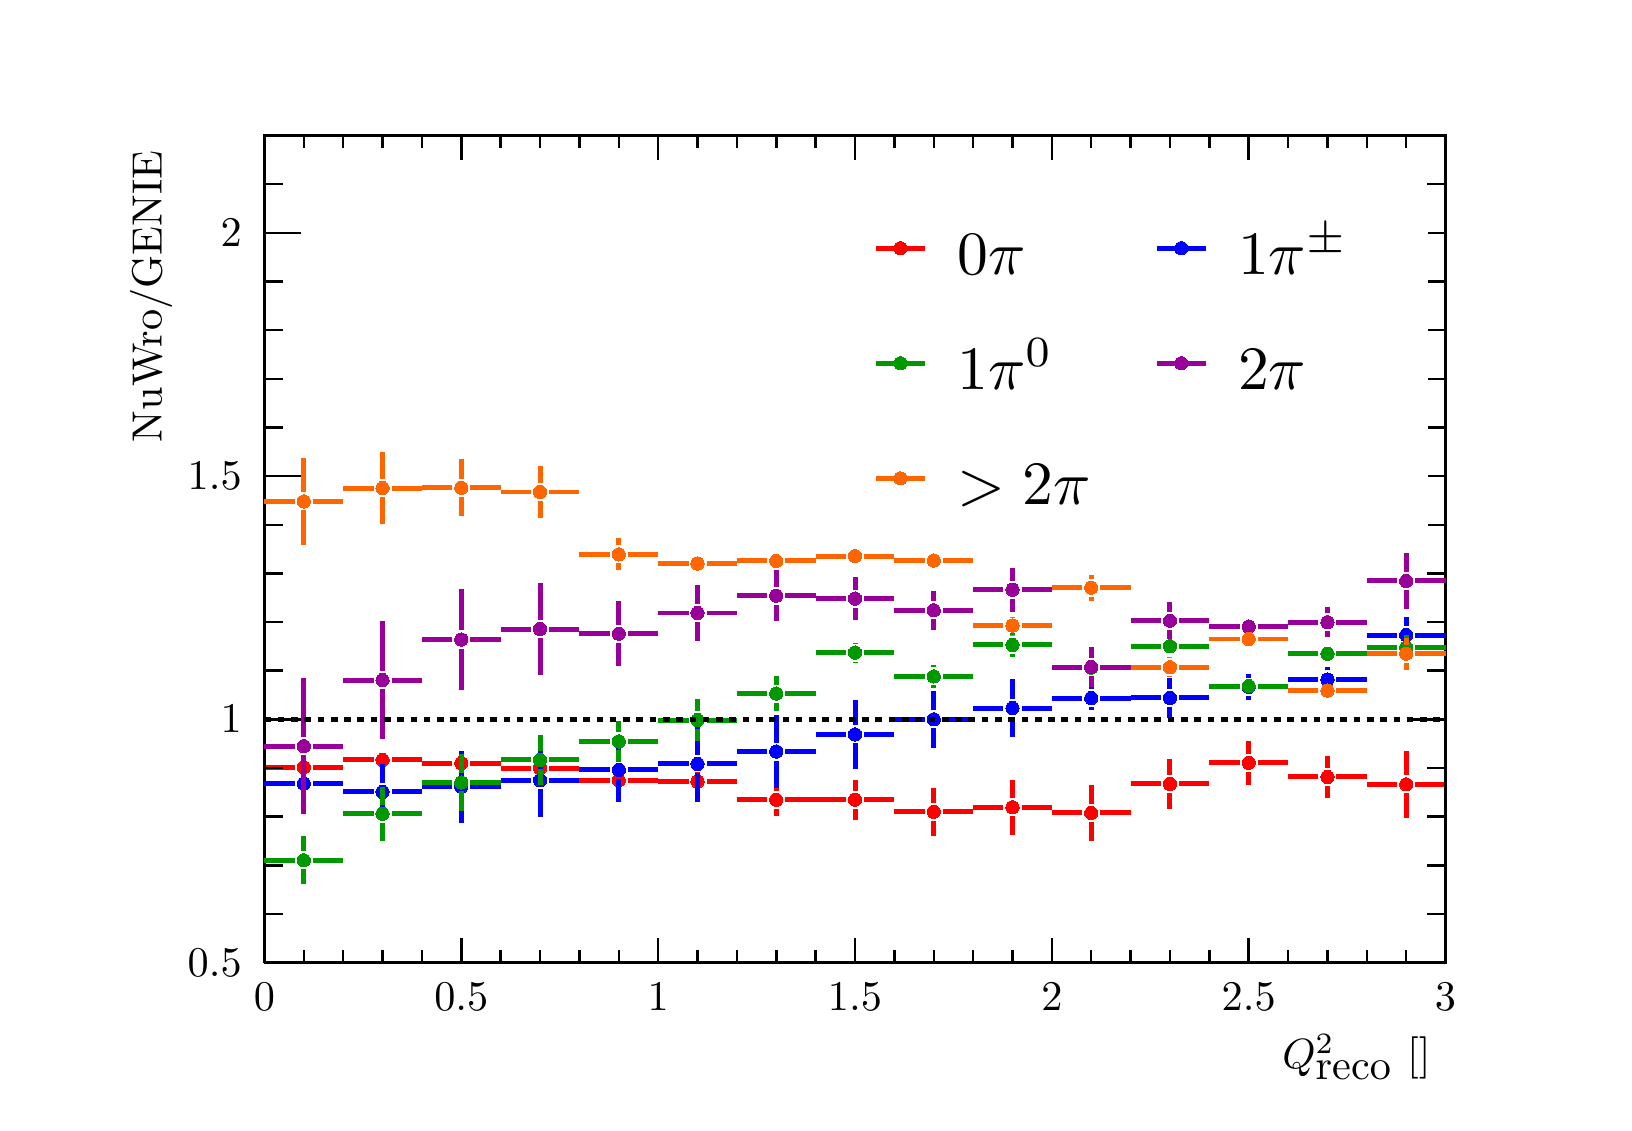
\begin{tikzpicture} 
\pgfdeclareplotmark{cross} {
\pgfpathmoveto{\pgfpoint{-0.3\pgfplotmarksize}{\pgfplotmarksize}}
\pgfpathlineto{\pgfpoint{+0.3\pgfplotmarksize}{\pgfplotmarksize}}
\pgfpathlineto{\pgfpoint{+0.3\pgfplotmarksize}{0.3\pgfplotmarksize}}
\pgfpathlineto{\pgfpoint{+1\pgfplotmarksize}{0.3\pgfplotmarksize}}
\pgfpathlineto{\pgfpoint{+1\pgfplotmarksize}{-0.3\pgfplotmarksize}}
\pgfpathlineto{\pgfpoint{+0.3\pgfplotmarksize}{-0.3\pgfplotmarksize}}
\pgfpathlineto{\pgfpoint{+0.3\pgfplotmarksize}{-1.\pgfplotmarksize}}
\pgfpathlineto{\pgfpoint{-0.3\pgfplotmarksize}{-1.\pgfplotmarksize}}
\pgfpathlineto{\pgfpoint{-0.3\pgfplotmarksize}{-0.3\pgfplotmarksize}}
\pgfpathlineto{\pgfpoint{-1.\pgfplotmarksize}{-0.3\pgfplotmarksize}}
\pgfpathlineto{\pgfpoint{-1.\pgfplotmarksize}{0.3\pgfplotmarksize}}
\pgfpathlineto{\pgfpoint{-0.3\pgfplotmarksize}{0.3\pgfplotmarksize}}
\pgfpathclose
\pgfusepathqstroke
}
\pgfdeclareplotmark{cross*} {
\pgfpathmoveto{\pgfpoint{-0.3\pgfplotmarksize}{\pgfplotmarksize}}
\pgfpathlineto{\pgfpoint{+0.3\pgfplotmarksize}{\pgfplotmarksize}}
\pgfpathlineto{\pgfpoint{+0.3\pgfplotmarksize}{0.3\pgfplotmarksize}}
\pgfpathlineto{\pgfpoint{+1\pgfplotmarksize}{0.3\pgfplotmarksize}}
\pgfpathlineto{\pgfpoint{+1\pgfplotmarksize}{-0.3\pgfplotmarksize}}
\pgfpathlineto{\pgfpoint{+0.3\pgfplotmarksize}{-0.3\pgfplotmarksize}}
\pgfpathlineto{\pgfpoint{+0.3\pgfplotmarksize}{-1.\pgfplotmarksize}}
\pgfpathlineto{\pgfpoint{-0.3\pgfplotmarksize}{-1.\pgfplotmarksize}}
\pgfpathlineto{\pgfpoint{-0.3\pgfplotmarksize}{-0.3\pgfplotmarksize}}
\pgfpathlineto{\pgfpoint{-1.\pgfplotmarksize}{-0.3\pgfplotmarksize}}
\pgfpathlineto{\pgfpoint{-1.\pgfplotmarksize}{0.3\pgfplotmarksize}}
\pgfpathlineto{\pgfpoint{-0.3\pgfplotmarksize}{0.3\pgfplotmarksize}}
\pgfpathclose
\pgfusepathqfillstroke
}
\pgfdeclareplotmark{newstar} {
\pgfpathmoveto{\pgfqpoint{0pt}{\pgfplotmarksize}}
\pgfpathlineto{\pgfqpointpolar{44}{0.5\pgfplotmarksize}}
\pgfpathlineto{\pgfqpointpolar{18}{\pgfplotmarksize}}
\pgfpathlineto{\pgfqpointpolar{-20}{0.5\pgfplotmarksize}}
\pgfpathlineto{\pgfqpointpolar{-54}{\pgfplotmarksize}}
\pgfpathlineto{\pgfqpointpolar{-90}{0.5\pgfplotmarksize}}
\pgfpathlineto{\pgfqpointpolar{234}{\pgfplotmarksize}}
\pgfpathlineto{\pgfqpointpolar{198}{0.5\pgfplotmarksize}}
\pgfpathlineto{\pgfqpointpolar{162}{\pgfplotmarksize}}
\pgfpathlineto{\pgfqpointpolar{134}{0.5\pgfplotmarksize}}
\pgfpathclose
\pgfusepathqstroke
}
\pgfdeclareplotmark{newstar*} {
\pgfpathmoveto{\pgfqpoint{0pt}{\pgfplotmarksize}}
\pgfpathlineto{\pgfqpointpolar{44}{0.5\pgfplotmarksize}}
\pgfpathlineto{\pgfqpointpolar{18}{\pgfplotmarksize}}
\pgfpathlineto{\pgfqpointpolar{-20}{0.5\pgfplotmarksize}}
\pgfpathlineto{\pgfqpointpolar{-54}{\pgfplotmarksize}}
\pgfpathlineto{\pgfqpointpolar{-90}{0.5\pgfplotmarksize}}
\pgfpathlineto{\pgfqpointpolar{234}{\pgfplotmarksize}}
\pgfpathlineto{\pgfqpointpolar{198}{0.5\pgfplotmarksize}}
\pgfpathlineto{\pgfqpointpolar{162}{\pgfplotmarksize}}
\pgfpathlineto{\pgfqpointpolar{134}{0.5\pgfplotmarksize}}
\pgfpathclose
\pgfusepathqfillstroke
}
\definecolor{c}{rgb}{1,1,1};
\draw [color=c, fill=c] (0,0) rectangle (20,13.639);
\draw [color=c, fill=c] (3,1.77307) rectangle (18,12.2751);
\definecolor{c}{rgb}{0,0,0};
\draw [c,line width=0.9] (3,1.77307) -- (3,12.2751) -- (18,12.2751) -- (18,1.77307) -- (3,1.77307);
\definecolor{c}{rgb}{1,1,1};
\draw [color=c, fill=c] (3,1.77307) rectangle (18,12.2751);
\definecolor{c}{rgb}{0,0,0};
\draw [c,line width=0.9] (3,1.77307) -- (3,12.2751) -- (18,12.2751) -- (18,1.77307) -- (3,1.77307);
\definecolor{c}{rgb}{1,0,0};
\draw [c,line width=1.8] (3,4.25421) -- (3.38539,4.25421);
\draw [c,line width=1.8] (3.61461,4.25421) -- (4,4.25421);
\foreach \P in {(3.5,4.25421)}{\draw[mark options={color=c,fill=c},mark size=2.402402pt, line width=0.000000pt, mark=*] plot coordinates {\P};}
\draw [c,line width=1.8] (4,4.34567) -- (4.38539,4.34567);
\draw [c,line width=1.8] (4.61461,4.34567) -- (5,4.34567);
\foreach \P in {(4.5,4.34567)}{\draw[mark options={color=c,fill=c},mark size=2.402402pt, line width=0.000000pt, mark=*] plot coordinates {\P};}
\draw [c,line width=1.8] (5,4.30631) -- (5.38539,4.30631);
\draw [c,line width=1.8] (5.61461,4.30631) -- (6,4.30631);
\foreach \P in {(5.5,4.30631)}{\draw[mark options={color=c,fill=c},mark size=2.402402pt, line width=0.000000pt, mark=*] plot coordinates {\P};}
\draw [c,line width=1.8] (6,4.24171) -- (6.38539,4.24171);
\draw [c,line width=1.8] (6.61461,4.24171) -- (7,4.24171);
\foreach \P in {(6.5,4.24171)}{\draw[mark options={color=c,fill=c},mark size=2.402402pt, line width=0.000000pt, mark=*] plot coordinates {\P};}
\draw [c,line width=1.8] (7,4.08889) -- (7.38539,4.08889);
\draw [c,line width=1.8] (7.61461,4.08889) -- (8,4.08889);
\foreach \P in {(7.5,4.08889)}{\draw[mark options={color=c,fill=c},mark size=2.402402pt, line width=0.000000pt, mark=*] plot coordinates {\P};}
\draw [c,line width=1.8] (8.5,3.95128) -- (8.5,3.95761);
\draw [c,line width=1.8] (8.5,4.18684) -- (8.5,4.19317);
\draw [c,line width=1.8] (8,4.07222) -- (8.38539,4.07222);
\draw [c,line width=1.8] (8.61461,4.07222) -- (9,4.07222);
\foreach \P in {(8.5,4.07222)}{\draw[mark options={color=c,fill=c},mark size=2.402402pt, line width=0.000000pt, mark=*] plot coordinates {\P};}
\draw [c,line width=1.8] (9.5,3.63206) -- (9.5,3.72656);
\draw [c,line width=1.8] (9.5,3.95578) -- (9.5,4.05028);
\draw [c,line width=1.8] (9,3.84117) -- (9.38539,3.84117);
\draw [c,line width=1.8] (9.61461,3.84117) -- (10,3.84117);
\foreach \P in {(9.5,3.84117)}{\draw[mark options={color=c,fill=c},mark size=2.402402pt, line width=0.000000pt, mark=*] plot coordinates {\P};}
\draw [c,line width=1.8] (10.5,3.58793) -- (10.5,3.72697);
\draw [c,line width=1.8] (10.5,3.9562) -- (10.5,4.09523);
\draw [c,line width=1.8] (10,3.84158) -- (10.3854,3.84158);
\draw [c,line width=1.8] (10.6146,3.84158) -- (11,3.84158);
\foreach \P in {(10.5,3.84158)}{\draw[mark options={color=c,fill=c},mark size=2.402402pt, line width=0.000000pt, mark=*] plot coordinates {\P};}
\draw [c,line width=1.8] (11.5,3.38105) -- (11.5,3.57398);
\draw [c,line width=1.8] (11.5,3.8032) -- (11.5,3.99612);
\draw [c,line width=1.8] (11,3.68859) -- (11.3854,3.68859);
\draw [c,line width=1.8] (11.6146,3.68859) -- (12,3.68859);
\foreach \P in {(11.5,3.68859)}{\draw[mark options={color=c,fill=c},mark size=2.402402pt, line width=0.000000pt, mark=*] plot coordinates {\P};}
\draw [c,line width=1.8] (12.5,3.39304) -- (12.5,3.62991);
\draw [c,line width=1.8] (12.5,3.85914) -- (12.5,4.09601);
\draw [c,line width=1.8] (12,3.74452) -- (12.3854,3.74452);
\draw [c,line width=1.8] (12.6146,3.74452) -- (13,3.74452);
\foreach \P in {(12.5,3.74452)}{\draw[mark options={color=c,fill=c},mark size=2.402402pt, line width=0.000000pt, mark=*] plot coordinates {\P};}
\draw [c,line width=1.8] (13.5,3.31572) -- (13.5,3.55841);
\draw [c,line width=1.8] (13.5,3.78764) -- (13.5,4.03034);
\draw [c,line width=1.8] (13,3.67303) -- (13.3854,3.67303);
\draw [c,line width=1.8] (13.6146,3.67303) -- (14,3.67303);
\foreach \P in {(13.5,3.67303)}{\draw[mark options={color=c,fill=c},mark size=2.402402pt, line width=0.000000pt, mark=*] plot coordinates {\P};}
\draw [c,line width=1.8] (14.5,3.72735) -- (14.5,3.92631);
\draw [c,line width=1.8] (14.5,4.15553) -- (14.5,4.35448);
\draw [c,line width=1.8] (14,4.04092) -- (14.3854,4.04092);
\draw [c,line width=1.8] (14.6146,4.04092) -- (15,4.04092);
\foreach \P in {(14.5,4.04092)}{\draw[mark options={color=c,fill=c},mark size=2.402402pt, line width=0.000000pt, mark=*] plot coordinates {\P};}
\draw [c,line width=1.8] (15.5,4.02951) -- (15.5,4.19558);
\draw [c,line width=1.8] (15.5,4.42481) -- (15.5,4.59088);
\draw [c,line width=1.8] (15,4.3102) -- (15.3854,4.3102);
\draw [c,line width=1.8] (15.6146,4.3102) -- (16,4.3102);
\foreach \P in {(15.5,4.3102)}{\draw[mark options={color=c,fill=c},mark size=2.402402pt, line width=0.000000pt, mark=*] plot coordinates {\P};}
\draw [c,line width=1.8] (16.5,3.85896) -- (16.5,4.01508);
\draw [c,line width=1.8] (16.5,4.24431) -- (16.5,4.40042);
\draw [c,line width=1.8] (16,4.12969) -- (16.3854,4.12969);
\draw [c,line width=1.8] (16.6146,4.12969) -- (17,4.12969);
\foreach \P in {(16.5,4.12969)}{\draw[mark options={color=c,fill=c},mark size=2.402402pt, line width=0.000000pt, mark=*] plot coordinates {\P};}
\draw [c,line width=1.8] (17.5,3.61236) -- (17.5,3.92183);
\draw [c,line width=1.8] (17.5,4.15105) -- (17.5,4.46052);
\draw [c,line width=1.8] (17,4.03644) -- (17.3854,4.03644);
\draw [c,line width=1.8] (17.6146,4.03644) -- (18,4.03644);
\foreach \P in {(17.5,4.03644)}{\draw[mark options={color=c,fill=c},mark size=2.402402pt, line width=0.000000pt, mark=*] plot coordinates {\P};}
\definecolor{c}{rgb}{0,0,0};
\draw [c,line width=0.9] (3,1.77307) -- (18,1.77307);
\draw [c,line width=0.9] (3,2.07994) -- (3,1.77307);
\draw [c,line width=0.9] (3.5,1.9265) -- (3.5,1.77307);
\draw [c,line width=0.9] (4,1.9265) -- (4,1.77307);
\draw [c,line width=0.9] (4.5,1.9265) -- (4.5,1.77307);
\draw [c,line width=0.9] (5,1.9265) -- (5,1.77307);
\draw [c,line width=0.9] (5.5,2.07994) -- (5.5,1.77307);
\draw [c,line width=0.9] (6,1.9265) -- (6,1.77307);
\draw [c,line width=0.9] (6.5,1.9265) -- (6.5,1.77307);
\draw [c,line width=0.9] (7,1.9265) -- (7,1.77307);
\draw [c,line width=0.9] (7.5,1.9265) -- (7.5,1.77307);
\draw [c,line width=0.9] (8,2.07994) -- (8,1.77307);
\draw [c,line width=0.9] (8.5,1.9265) -- (8.5,1.77307);
\draw [c,line width=0.9] (9,1.9265) -- (9,1.77307);
\draw [c,line width=0.9] (9.5,1.9265) -- (9.5,1.77307);
\draw [c,line width=0.9] (10,1.9265) -- (10,1.77307);
\draw [c,line width=0.9] (10.5,2.07994) -- (10.5,1.77307);
\draw [c,line width=0.9] (11,1.9265) -- (11,1.77307);
\draw [c,line width=0.9] (11.5,1.9265) -- (11.5,1.77307);
\draw [c,line width=0.9] (12,1.9265) -- (12,1.77307);
\draw [c,line width=0.9] (12.5,1.9265) -- (12.5,1.77307);
\draw [c,line width=0.9] (13,2.07994) -- (13,1.77307);
\draw [c,line width=0.9] (13.5,1.9265) -- (13.5,1.77307);
\draw [c,line width=0.9] (14,1.9265) -- (14,1.77307);
\draw [c,line width=0.9] (14.5,1.9265) -- (14.5,1.77307);
\draw [c,line width=0.9] (15,1.9265) -- (15,1.77307);
\draw [c,line width=0.9] (15.5,2.07994) -- (15.5,1.77307);
\draw [c,line width=0.9] (16,1.9265) -- (16,1.77307);
\draw [c,line width=0.9] (16.5,1.9265) -- (16.5,1.77307);
\draw [c,line width=0.9] (17,1.9265) -- (17,1.77307);
\draw [c,line width=0.9] (17.5,1.9265) -- (17.5,1.77307);
\draw [c,line width=0.9] (18,2.07994) -- (18,1.77307);
\draw [c,line width=0.9] (18,2.07994) -- (18,1.77307);
\draw [anchor=base] (3,1.15931) node[scale=1.52731, color=c, rotate=0]{0};
\draw [anchor=base] (5.5,1.15931) node[scale=1.52731, color=c, rotate=0]{0.5};
\draw [anchor=base] (8,1.15931) node[scale=1.52731, color=c, rotate=0]{1};
\draw [anchor=base] (10.5,1.15931) node[scale=1.52731, color=c, rotate=0]{1.5};
\draw [anchor=base] (13,1.15931) node[scale=1.52731, color=c, rotate=0]{2};
\draw [anchor=base] (15.5,1.15931) node[scale=1.52731, color=c, rotate=0]{2.5};
\draw [anchor=base] (18,1.15931) node[scale=1.52731, color=c, rotate=0]{3};
\draw [anchor= east] (18,0.572837) node[scale=1.52731, color=c, rotate=0]{$Q^{2}_{\textrm{reco}}$ [\si{\GeV\squared}] };
\draw [c,line width=0.9] (3,12.2751) -- (18,12.2751);
\draw [c,line width=0.9] (3,11.9682) -- (3,12.2751);
\draw [c,line width=0.9] (3.5,12.1216) -- (3.5,12.2751);
\draw [c,line width=0.9] (4,12.1216) -- (4,12.2751);
\draw [c,line width=0.9] (4.5,12.1216) -- (4.5,12.2751);
\draw [c,line width=0.9] (5,12.1216) -- (5,12.2751);
\draw [c,line width=0.9] (5.5,11.9682) -- (5.5,12.2751);
\draw [c,line width=0.9] (6,12.1216) -- (6,12.2751);
\draw [c,line width=0.9] (6.5,12.1216) -- (6.5,12.2751);
\draw [c,line width=0.9] (7,12.1216) -- (7,12.2751);
\draw [c,line width=0.9] (7.5,12.1216) -- (7.5,12.2751);
\draw [c,line width=0.9] (8,11.9682) -- (8,12.2751);
\draw [c,line width=0.9] (8.5,12.1216) -- (8.5,12.2751);
\draw [c,line width=0.9] (9,12.1216) -- (9,12.2751);
\draw [c,line width=0.9] (9.5,12.1216) -- (9.5,12.2751);
\draw [c,line width=0.9] (10,12.1216) -- (10,12.2751);
\draw [c,line width=0.9] (10.5,11.9682) -- (10.5,12.2751);
\draw [c,line width=0.9] (11,12.1216) -- (11,12.2751);
\draw [c,line width=0.9] (11.5,12.1216) -- (11.5,12.2751);
\draw [c,line width=0.9] (12,12.1216) -- (12,12.2751);
\draw [c,line width=0.9] (12.5,12.1216) -- (12.5,12.2751);
\draw [c,line width=0.9] (13,11.9682) -- (13,12.2751);
\draw [c,line width=0.9] (13.5,12.1216) -- (13.5,12.2751);
\draw [c,line width=0.9] (14,12.1216) -- (14,12.2751);
\draw [c,line width=0.9] (14.5,12.1216) -- (14.5,12.2751);
\draw [c,line width=0.9] (15,12.1216) -- (15,12.2751);
\draw [c,line width=0.9] (15.5,11.9682) -- (15.5,12.2751);
\draw [c,line width=0.9] (16,12.1216) -- (16,12.2751);
\draw [c,line width=0.9] (16.5,12.1216) -- (16.5,12.2751);
\draw [c,line width=0.9] (17,12.1216) -- (17,12.2751);
\draw [c,line width=0.9] (17.5,12.1216) -- (17.5,12.2751);
\draw [c,line width=0.9] (18,11.9682) -- (18,12.2751);
\draw [c,line width=0.9] (18,11.9682) -- (18,12.2751);
\draw [c,line width=0.9] (3,1.77307) -- (3,12.2751);
\draw [c,line width=0.9] (3.462,1.77307) -- (3,1.77307);
\draw [c,line width=0.9] (3.231,2.39083) -- (3,2.39083);
\draw [c,line width=0.9] (3.231,3.0086) -- (3,3.0086);
\draw [c,line width=0.9] (3.231,3.62636) -- (3,3.62636);
\draw [c,line width=0.9] (3.231,4.24413) -- (3,4.24413);
\draw [c,line width=0.9] (3.462,4.86189) -- (3,4.86189);
\draw [c,line width=0.9] (3.231,5.47966) -- (3,5.47966);
\draw [c,line width=0.9] (3.231,6.09742) -- (3,6.09742);
\draw [c,line width=0.9] (3.231,6.71519) -- (3,6.71519);
\draw [c,line width=0.9] (3.231,7.33295) -- (3,7.33295);
\draw [c,line width=0.9] (3.462,7.95072) -- (3,7.95072);
\draw [c,line width=0.9] (3.231,8.56848) -- (3,8.56848);
\draw [c,line width=0.9] (3.231,9.18625) -- (3,9.18625);
\draw [c,line width=0.9] (3.231,9.80401) -- (3,9.80401);
\draw [c,line width=0.9] (3.231,10.4218) -- (3,10.4218);
\draw [c,line width=0.9] (3.462,11.0395) -- (3,11.0395);
\draw [c,line width=0.9] (3.462,11.0395) -- (3,11.0395);
\draw [c,line width=0.9] (3.231,11.6573) -- (3,11.6573);
\draw [c,line width=0.9] (3.231,12.2751) -- (3,12.2751);
\draw [anchor= east] (2.9,1.77307) node[scale=1.52731, color=c, rotate=0]{0.5};
\draw [anchor= east] (2.9,4.86189) node[scale=1.52731, color=c, rotate=0]{1};
\draw [anchor= east] (2.9,7.95072) node[scale=1.52731, color=c, rotate=0]{1.5};
\draw [anchor= east] (2.9,11.0395) node[scale=1.52731, color=c, rotate=0]{2};
\draw [anchor= east] (1.56,12.2751) node[scale=1.52731, color=c, rotate=90]{ NuWro/GENIE};
\draw [c,line width=0.9] (18,1.77307) -- (18,12.2751);
\draw [c,line width=0.9] (17.538,1.77307) -- (18,1.77307);
\draw [c,line width=0.9] (17.769,2.39083) -- (18,2.39083);
\draw [c,line width=0.9] (17.769,3.0086) -- (18,3.0086);
\draw [c,line width=0.9] (17.769,3.62636) -- (18,3.62636);
\draw [c,line width=0.9] (17.769,4.24413) -- (18,4.24413);
\draw [c,line width=0.9] (17.538,4.86189) -- (18,4.86189);
\draw [c,line width=0.9] (17.769,5.47966) -- (18,5.47966);
\draw [c,line width=0.9] (17.769,6.09742) -- (18,6.09742);
\draw [c,line width=0.9] (17.769,6.71519) -- (18,6.71519);
\draw [c,line width=0.9] (17.769,7.33295) -- (18,7.33295);
\draw [c,line width=0.9] (17.538,7.95072) -- (18,7.95072);
\draw [c,line width=0.9] (17.769,8.56848) -- (18,8.56848);
\draw [c,line width=0.9] (17.769,9.18625) -- (18,9.18625);
\draw [c,line width=0.9] (17.769,9.80401) -- (18,9.80401);
\draw [c,line width=0.9] (17.769,10.4218) -- (18,10.4218);
\draw [c,line width=0.9] (17.538,11.0395) -- (18,11.0395);
\draw [c,line width=0.9] (17.538,11.0395) -- (18,11.0395);
\draw [c,line width=0.9] (17.769,11.6573) -- (18,11.6573);
\draw [c,line width=0.9] (17.769,12.2751) -- (18,12.2751);
\definecolor{c}{rgb}{0,0,1};
\draw [c,line width=1.8] (3.5,3.85564) -- (3.5,3.93025);
\draw [c,line width=1.8] (3.5,4.15947) -- (3.5,4.23409);
\draw [c,line width=1.8] (3,4.04486) -- (3.38539,4.04486);
\draw [c,line width=1.8] (3.61461,4.04486) -- (4,4.04486);
\foreach \P in {(3.5,4.04486)}{\draw[mark options={color=c,fill=c},mark size=2.402402pt, line width=0.000000pt, mark=*] plot coordinates {\P};}
\draw [c,line width=1.8] (4.5,3.58177) -- (4.5,3.82528);
\draw [c,line width=1.8] (4.5,4.05451) -- (4.5,4.29802);
\draw [c,line width=1.8] (4,3.93989) -- (4.38539,3.93989);
\draw [c,line width=1.8] (4.61461,3.93989) -- (5,3.93989);
\foreach \P in {(4.5,3.93989)}{\draw[mark options={color=c,fill=c},mark size=2.402402pt, line width=0.000000pt, mark=*] plot coordinates {\P};}
\draw [c,line width=1.8] (5.5,3.55128) -- (5.5,3.892);
\draw [c,line width=1.8] (5.5,4.12123) -- (5.5,4.46194);
\draw [c,line width=1.8] (5,4.00661) -- (5.38539,4.00661);
\draw [c,line width=1.8] (5.61461,4.00661) -- (6,4.00661);
\foreach \P in {(5.5,4.00661)}{\draw[mark options={color=c,fill=c},mark size=2.402402pt, line width=0.000000pt, mark=*] plot coordinates {\P};}
\draw [c,line width=1.8] (6.5,3.62757) -- (6.5,3.97413);
\draw [c,line width=1.8] (6.5,4.20336) -- (6.5,4.54993);
\draw [c,line width=1.8] (6,4.08875) -- (6.38539,4.08875);
\draw [c,line width=1.8] (6.61461,4.08875) -- (7,4.08875);
\foreach \P in {(6.5,4.08875)}{\draw[mark options={color=c,fill=c},mark size=2.402402pt, line width=0.000000pt, mark=*] plot coordinates {\P};}
\draw [c,line width=1.8] (7.5,3.81352) -- (7.5,4.10518);
\draw [c,line width=1.8] (7.5,4.3344) -- (7.5,4.62606);
\draw [c,line width=1.8] (7,4.21979) -- (7.38539,4.21979);
\draw [c,line width=1.8] (7.61461,4.21979) -- (8,4.21979);
\foreach \P in {(7.5,4.21979)}{\draw[mark options={color=c,fill=c},mark size=2.402402pt, line width=0.000000pt, mark=*] plot coordinates {\P};}
\draw [c,line width=1.8] (8.5,3.81693) -- (8.5,4.18106);
\draw [c,line width=1.8] (8.5,4.41029) -- (8.5,4.77442);
\draw [c,line width=1.8] (8,4.29568) -- (8.38539,4.29568);
\draw [c,line width=1.8] (8.61461,4.29568) -- (9,4.29568);
\foreach \P in {(8.5,4.29568)}{\draw[mark options={color=c,fill=c},mark size=2.402402pt, line width=0.000000pt, mark=*] plot coordinates {\P};}
\draw [c,line width=1.8] (9.5,3.98934) -- (9.5,4.33832);
\draw [c,line width=1.8] (9.5,4.56755) -- (9.5,4.91652);
\draw [c,line width=1.8] (9,4.45293) -- (9.38539,4.45293);
\draw [c,line width=1.8] (9.61461,4.45293) -- (10,4.45293);
\foreach \P in {(9.5,4.45293)}{\draw[mark options={color=c,fill=c},mark size=2.402402pt, line width=0.000000pt, mark=*] plot coordinates {\P};}
\draw [c,line width=1.8] (10.5,4.23524) -- (10.5,4.55537);
\draw [c,line width=1.8] (10.5,4.7846) -- (10.5,5.10473);
\draw [c,line width=1.8] (10,4.66999) -- (10.3854,4.66999);
\draw [c,line width=1.8] (10.6146,4.66999) -- (11,4.66999);
\foreach \P in {(10.5,4.66999)}{\draw[mark options={color=c,fill=c},mark size=2.402402pt, line width=0.000000pt, mark=*] plot coordinates {\P};}
\draw [c,line width=1.8] (11.5,4.49798) -- (11.5,4.74711);
\draw [c,line width=1.8] (11.5,4.97634) -- (11.5,5.22547);
\draw [c,line width=1.8] (11,4.86172) -- (11.3854,4.86172);
\draw [c,line width=1.8] (11.6146,4.86172) -- (12,4.86172);
\foreach \P in {(11.5,4.86172)}{\draw[mark options={color=c,fill=c},mark size=2.402402pt, line width=0.000000pt, mark=*] plot coordinates {\P};}
\draw [c,line width=1.8] (12.5,4.63848) -- (12.5,4.89032);
\draw [c,line width=1.8] (12.5,5.11954) -- (12.5,5.37138);
\draw [c,line width=1.8] (12,5.00493) -- (12.3854,5.00493);
\draw [c,line width=1.8] (12.6146,5.00493) -- (13,5.00493);
\foreach \P in {(12.5,5.00493)}{\draw[mark options={color=c,fill=c},mark size=2.402402pt, line width=0.000000pt, mark=*] plot coordinates {\P};}
\draw [c,line width=1.8] (13.5,4.97669) -- (13.5,5.01721);
\draw [c,line width=1.8] (13.5,5.24644) -- (13.5,5.28695);
\draw [c,line width=1.8] (13,5.13182) -- (13.3854,5.13182);
\draw [c,line width=1.8] (13.6146,5.13182) -- (14,5.13182);
\foreach \P in {(13.5,5.13182)}{\draw[mark options={color=c,fill=c},mark size=2.402402pt, line width=0.000000pt, mark=*] plot coordinates {\P};}
\draw [c,line width=1.8] (14.5,4.88157) -- (14.5,5.01984);
\draw [c,line width=1.8] (14.5,5.24906) -- (14.5,5.38732);
\draw [c,line width=1.8] (14,5.13445) -- (14.3854,5.13445);
\draw [c,line width=1.8] (14.6146,5.13445) -- (15,5.13445);
\foreach \P in {(14.5,5.13445)}{\draw[mark options={color=c,fill=c},mark size=2.402402pt, line width=0.000000pt, mark=*] plot coordinates {\P};}
\draw [c,line width=1.8] (15.5,5.10808) -- (15.5,5.1601);
\draw [c,line width=1.8] (15.5,5.38933) -- (15.5,5.44135);
\draw [c,line width=1.8] (15,5.27471) -- (15.3854,5.27471);
\draw [c,line width=1.8] (15.6146,5.27471) -- (16,5.27471);
\foreach \P in {(15.5,5.27471)}{\draw[mark options={color=c,fill=c},mark size=2.402402pt, line width=0.000000pt, mark=*] plot coordinates {\P};}
\draw [c,line width=1.8] (16.5,5.2049) -- (16.5,5.25334);
\draw [c,line width=1.8] (16.5,5.48257) -- (16.5,5.531);
\draw [c,line width=1.8] (16,5.36795) -- (16.3854,5.36795);
\draw [c,line width=1.8] (16.6146,5.36795) -- (17,5.36795);
\foreach \P in {(16.5,5.36795)}{\draw[mark options={color=c,fill=c},mark size=2.402402pt, line width=0.000000pt, mark=*] plot coordinates {\P};}
\draw [c,line width=1.8] (17.5,5.70018) -- (17.5,5.81797);
\draw [c,line width=1.8] (17.5,6.0472) -- (17.5,6.16499);
\draw [c,line width=1.8] (17,5.93258) -- (17.3854,5.93258);
\draw [c,line width=1.8] (17.6146,5.93258) -- (18,5.93258);
\foreach \P in {(17.5,5.93258)}{\draw[mark options={color=c,fill=c},mark size=2.402402pt, line width=0.000000pt, mark=*] plot coordinates {\P};}
\definecolor{c}{rgb}{0,0.6,0};
\draw [c,line width=1.8] (3.5,2.76788) -- (3.5,2.95756);
\draw [c,line width=1.8] (3.5,3.18679) -- (3.5,3.37647);
\draw [c,line width=1.8] (3,3.07217) -- (3.38539,3.07217);
\draw [c,line width=1.8] (3.61461,3.07217) -- (4,3.07217);
\foreach \P in {(3.5,3.07217)}{\draw[mark options={color=c,fill=c},mark size=2.402402pt, line width=0.000000pt, mark=*] plot coordinates {\P};}
\draw [c,line width=1.8] (4.5,3.32244) -- (4.5,3.54829);
\draw [c,line width=1.8] (4.5,3.77752) -- (4.5,4.00337);
\draw [c,line width=1.8] (4,3.6629) -- (4.38539,3.6629);
\draw [c,line width=1.8] (4.61461,3.6629) -- (5,3.6629);
\foreach \P in {(4.5,3.6629)}{\draw[mark options={color=c,fill=c},mark size=2.402402pt, line width=0.000000pt, mark=*] plot coordinates {\P};}
\draw [c,line width=1.8] (5.5,3.70004) -- (5.5,3.94594);
\draw [c,line width=1.8] (5.5,4.17516) -- (5.5,4.42106);
\draw [c,line width=1.8] (5,4.06055) -- (5.38539,4.06055);
\draw [c,line width=1.8] (5.61461,4.06055) -- (6,4.06055);
\foreach \P in {(5.5,4.06055)}{\draw[mark options={color=c,fill=c},mark size=2.402402pt, line width=0.000000pt, mark=*] plot coordinates {\P};}
\draw [c,line width=1.8] (6.5,4.02444) -- (6.5,4.23098);
\draw [c,line width=1.8] (6.5,4.46021) -- (6.5,4.66675);
\draw [c,line width=1.8] (6,4.3456) -- (6.38539,4.3456);
\draw [c,line width=1.8] (6.61461,4.3456) -- (7,4.3456);
\foreach \P in {(6.5,4.3456)}{\draw[mark options={color=c,fill=c},mark size=2.402402pt, line width=0.000000pt, mark=*] plot coordinates {\P};}
\draw [c,line width=1.8] (7.5,4.3251) -- (7.5,4.46706);
\draw [c,line width=1.8] (7.5,4.69629) -- (7.5,4.83825);
\draw [c,line width=1.8] (7,4.58167) -- (7.38539,4.58167);
\draw [c,line width=1.8] (7.61461,4.58167) -- (8,4.58167);
\foreach \P in {(7.5,4.58167)}{\draw[mark options={color=c,fill=c},mark size=2.402402pt, line width=0.000000pt, mark=*] plot coordinates {\P};}
\draw [c,line width=1.8] (8.5,4.58307) -- (8.5,4.73735);
\draw [c,line width=1.8] (8.5,4.96658) -- (8.5,5.12086);
\draw [c,line width=1.8] (8,4.85196) -- (8.38539,4.85196);
\draw [c,line width=1.8] (8.61461,4.85196) -- (9,4.85196);
\foreach \P in {(8.5,4.85196)}{\draw[mark options={color=c,fill=c},mark size=2.402402pt, line width=0.000000pt, mark=*] plot coordinates {\P};}
\draw [c,line width=1.8] (9.5,4.96684) -- (9.5,5.07409);
\draw [c,line width=1.8] (9.5,5.30332) -- (9.5,5.41058);
\draw [c,line width=1.8] (9,5.18871) -- (9.38539,5.18871);
\draw [c,line width=1.8] (9.61461,5.18871) -- (10,5.18871);
\foreach \P in {(9.5,5.18871)}{\draw[mark options={color=c,fill=c},mark size=2.402402pt, line width=0.000000pt, mark=*] plot coordinates {\P};}
\draw [c,line width=1.8] (10.5,5.58259) -- (10.5,5.59515);
\draw [c,line width=1.8] (10.5,5.82437) -- (10.5,5.83693);
\draw [c,line width=1.8] (10,5.70976) -- (10.3854,5.70976);
\draw [c,line width=1.8] (10.6146,5.70976) -- (11,5.70976);
\foreach \P in {(10.5,5.70976)}{\draw[mark options={color=c,fill=c},mark size=2.402402pt, line width=0.000000pt, mark=*] plot coordinates {\P};}
\draw [c,line width=1.8] (11.5,5.26367) -- (11.5,5.29283);
\draw [c,line width=1.8] (11.5,5.52206) -- (11.5,5.55123);
\draw [c,line width=1.8] (11,5.40745) -- (11.3854,5.40745);
\draw [c,line width=1.8] (11.6146,5.40745) -- (12,5.40745);
\foreach \P in {(11.5,5.40745)}{\draw[mark options={color=c,fill=c},mark size=2.402402pt, line width=0.000000pt, mark=*] plot coordinates {\P};}
\draw [c,line width=1.8] (12.5,5.65917) -- (12.5,5.69177);
\draw [c,line width=1.8] (12.5,5.921) -- (12.5,5.95361);
\draw [c,line width=1.8] (12,5.80639) -- (12.3854,5.80639);
\draw [c,line width=1.8] (12.6146,5.80639) -- (13,5.80639);
\foreach \P in {(12.5,5.80639)}{\draw[mark options={color=c,fill=c},mark size=2.402402pt, line width=0.000000pt, mark=*] plot coordinates {\P};}
\draw [c,line width=1.8] (13,5.51858) -- (13.3854,5.51858);
\draw [c,line width=1.8] (13.6146,5.51858) -- (14,5.51858);
\foreach \P in {(13.5,5.51858)}{\draw[mark options={color=c,fill=c},mark size=2.402402pt, line width=0.000000pt, mark=*] plot coordinates {\P};}
\draw [c,line width=1.8] (14,5.79098) -- (14.3854,5.79098);
\draw [c,line width=1.8] (14.6146,5.79098) -- (15,5.79098);
\foreach \P in {(14.5,5.79098)}{\draw[mark options={color=c,fill=c},mark size=2.402402pt, line width=0.000000pt, mark=*] plot coordinates {\P};}
\draw [c,line width=1.8] (15,5.28459) -- (15.3854,5.28459);
\draw [c,line width=1.8] (15.6146,5.28459) -- (16,5.28459);
\foreach \P in {(15.5,5.28459)}{\draw[mark options={color=c,fill=c},mark size=2.402402pt, line width=0.000000pt, mark=*] plot coordinates {\P};}
\draw [c,line width=1.8] (16,5.6943) -- (16.3854,5.6943);
\draw [c,line width=1.8] (16.6146,5.6943) -- (17,5.6943);
\foreach \P in {(16.5,5.6943)}{\draw[mark options={color=c,fill=c},mark size=2.402402pt, line width=0.000000pt, mark=*] plot coordinates {\P};}
\draw [c,line width=1.8] (17.5,5.61317) -- (17.5,5.65889);
\draw [c,line width=1.8] (17.5,5.88811) -- (17.5,5.93383);
\draw [c,line width=1.8] (17,5.7735) -- (17.3854,5.7735);
\draw [c,line width=1.8] (17.6146,5.7735) -- (18,5.7735);
\foreach \P in {(17.5,5.7735)}{\draw[mark options={color=c,fill=c},mark size=2.402402pt, line width=0.000000pt, mark=*] plot coordinates {\P};}
\definecolor{c}{rgb}{0.6,0,0.6};
\draw [c,line width=1.8] (3.5,3.65904) -- (3.5,4.4065);
\draw [c,line width=1.8] (3.5,4.63573) -- (3.5,5.38318);
\draw [c,line width=1.8] (3,4.52111) -- (3.38539,4.52111);
\draw [c,line width=1.8] (3.61461,4.52111) -- (4,4.52111);
\foreach \P in {(3.5,4.52111)}{\draw[mark options={color=c,fill=c},mark size=2.402402pt, line width=0.000000pt, mark=*] plot coordinates {\P};}
\draw [c,line width=1.8] (4.5,4.60862) -- (4.5,5.24532);
\draw [c,line width=1.8] (4.5,5.47454) -- (4.5,6.11124);
\draw [c,line width=1.8] (4,5.35993) -- (4.38539,5.35993);
\draw [c,line width=1.8] (4.61461,5.35993) -- (5,5.35993);
\foreach \P in {(4.5,5.35993)}{\draw[mark options={color=c,fill=c},mark size=2.402402pt, line width=0.000000pt, mark=*] plot coordinates {\P};}
\draw [c,line width=1.8] (5.5,5.2307) -- (5.5,5.76088);
\draw [c,line width=1.8] (5.5,5.9901) -- (5.5,6.52028);
\draw [c,line width=1.8] (5,5.87549) -- (5.38539,5.87549);
\draw [c,line width=1.8] (5.61461,5.87549) -- (6,5.87549);
\foreach \P in {(5.5,5.87549)}{\draw[mark options={color=c,fill=c},mark size=2.402402pt, line width=0.000000pt, mark=*] plot coordinates {\P};}
\draw [c,line width=1.8] (6.5,5.41876) -- (6.5,5.8942);
\draw [c,line width=1.8] (6.5,6.12343) -- (6.5,6.59886);
\draw [c,line width=1.8] (6,6.00881) -- (6.38539,6.00881);
\draw [c,line width=1.8] (6.61461,6.00881) -- (7,6.00881);
\foreach \P in {(6.5,6.00881)}{\draw[mark options={color=c,fill=c},mark size=2.402402pt, line width=0.000000pt, mark=*] plot coordinates {\P};}
\draw [c,line width=1.8] (7.5,5.53892) -- (7.5,5.83474);
\draw [c,line width=1.8] (7.5,6.06397) -- (7.5,6.3598);
\draw [c,line width=1.8] (7,5.94936) -- (7.38539,5.94936);
\draw [c,line width=1.8] (7.61461,5.94936) -- (8,5.94936);
\foreach \P in {(7.5,5.94936)}{\draw[mark options={color=c,fill=c},mark size=2.402402pt, line width=0.000000pt, mark=*] plot coordinates {\P};}
\draw [c,line width=1.8] (8.5,5.86292) -- (8.5,6.0977);
\draw [c,line width=1.8] (8.5,6.32692) -- (8.5,6.5617);
\draw [c,line width=1.8] (8,6.21231) -- (8.38539,6.21231);
\draw [c,line width=1.8] (8.61461,6.21231) -- (9,6.21231);
\foreach \P in {(8.5,6.21231)}{\draw[mark options={color=c,fill=c},mark size=2.402402pt, line width=0.000000pt, mark=*] plot coordinates {\P};}
\draw [c,line width=1.8] (9.5,6.11151) -- (9.5,6.31766);
\draw [c,line width=1.8] (9.5,6.54689) -- (9.5,6.75304);
\draw [c,line width=1.8] (9,6.43227) -- (9.38539,6.43227);
\draw [c,line width=1.8] (9.61461,6.43227) -- (10,6.43227);
\foreach \P in {(9.5,6.43227)}{\draw[mark options={color=c,fill=c},mark size=2.402402pt, line width=0.000000pt, mark=*] plot coordinates {\P};}
\draw [c,line width=1.8] (10.5,6.11706) -- (10.5,6.28095);
\draw [c,line width=1.8] (10.5,6.51018) -- (10.5,6.67407);
\draw [c,line width=1.8] (10,6.39557) -- (10.3854,6.39557);
\draw [c,line width=1.8] (10.6146,6.39557) -- (11,6.39557);
\foreach \P in {(10.5,6.39557)}{\draw[mark options={color=c,fill=c},mark size=2.402402pt, line width=0.000000pt, mark=*] plot coordinates {\P};}
\draw [c,line width=1.8] (11.5,6.00011) -- (11.5,6.13244);
\draw [c,line width=1.8] (11.5,6.36167) -- (11.5,6.49401);
\draw [c,line width=1.8] (11,6.24706) -- (11.3854,6.24706);
\draw [c,line width=1.8] (11.6146,6.24706) -- (12,6.24706);
\foreach \P in {(11.5,6.24706)}{\draw[mark options={color=c,fill=c},mark size=2.402402pt, line width=0.000000pt, mark=*] plot coordinates {\P};}
\draw [c,line width=1.8] (12.5,6.23056) -- (12.5,6.39411);
\draw [c,line width=1.8] (12.5,6.62333) -- (12.5,6.78688);
\draw [c,line width=1.8] (12,6.50872) -- (12.3854,6.50872);
\draw [c,line width=1.8] (12.6146,6.50872) -- (13,6.50872);
\foreach \P in {(12.5,6.50872)}{\draw[mark options={color=c,fill=c},mark size=2.402402pt, line width=0.000000pt, mark=*] plot coordinates {\P};}
\draw [c,line width=1.8] (13.5,5.27082) -- (13.5,5.4117);
\draw [c,line width=1.8] (13.5,5.64093) -- (13.5,5.78181);
\draw [c,line width=1.8] (13,5.52632) -- (13.3854,5.52632);
\draw [c,line width=1.8] (13.6146,5.52632) -- (14,5.52632);
\foreach \P in {(13.5,5.52632)}{\draw[mark options={color=c,fill=c},mark size=2.402402pt, line width=0.000000pt, mark=*] plot coordinates {\P};}
\draw [c,line width=1.8] (14.5,5.88151) -- (14.5,5.99948);
\draw [c,line width=1.8] (14.5,6.2287) -- (14.5,6.34667);
\draw [c,line width=1.8] (14,6.11409) -- (14.3854,6.11409);
\draw [c,line width=1.8] (14.6146,6.11409) -- (15,6.11409);
\foreach \P in {(14.5,6.11409)}{\draw[mark options={color=c,fill=c},mark size=2.402402pt, line width=0.000000pt, mark=*] plot coordinates {\P};}
\draw [c,line width=1.8] (15,6.03899) -- (15.3854,6.03899);
\draw [c,line width=1.8] (15.6146,6.03899) -- (16,6.03899);
\foreach \P in {(15.5,6.03899)}{\draw[mark options={color=c,fill=c},mark size=2.402402pt, line width=0.000000pt, mark=*] plot coordinates {\P};}
\draw [c,line width=1.8] (16.5,5.90295) -- (16.5,5.97987);
\draw [c,line width=1.8] (16.5,6.2091) -- (16.5,6.28602);
\draw [c,line width=1.8] (16,6.09448) -- (16.3854,6.09448);
\draw [c,line width=1.8] (16.6146,6.09448) -- (17,6.09448);
\foreach \P in {(16.5,6.09448)}{\draw[mark options={color=c,fill=c},mark size=2.402402pt, line width=0.000000pt, mark=*] plot coordinates {\P};}
\draw [c,line width=1.8] (17.5,6.26807) -- (17.5,6.50446);
\draw [c,line width=1.8] (17.5,6.73369) -- (17.5,6.97007);
\draw [c,line width=1.8] (17,6.61907) -- (17.3854,6.61907);
\draw [c,line width=1.8] (17.6146,6.61907) -- (18,6.61907);
\foreach \P in {(17.5,6.61907)}{\draw[mark options={color=c,fill=c},mark size=2.402402pt, line width=0.000000pt, mark=*] plot coordinates {\P};}
\definecolor{c}{rgb}{1,0.4,0};
\draw [c,line width=1.8] (3.5,7.0761) -- (3.5,7.51515);
\draw [c,line width=1.8] (3.5,7.74437) -- (3.5,8.18343);
\draw [c,line width=1.8] (3,7.62976) -- (3.38539,7.62976);
\draw [c,line width=1.8] (3.61461,7.62976) -- (4,7.62976);
\foreach \P in {(3.5,7.62976)}{\draw[mark options={color=c,fill=c},mark size=2.402402pt, line width=0.000000pt, mark=*] plot coordinates {\P};}
\draw [c,line width=1.8] (4.5,7.33943) -- (4.5,7.68486);
\draw [c,line width=1.8] (4.5,7.91409) -- (4.5,8.25952);
\draw [c,line width=1.8] (4,7.79948) -- (4.38539,7.79948);
\draw [c,line width=1.8] (4.61461,7.79948) -- (5,7.79948);
\foreach \P in {(4.5,7.79948)}{\draw[mark options={color=c,fill=c},mark size=2.402402pt, line width=0.000000pt, mark=*] plot coordinates {\P};}
\draw [c,line width=1.8] (5.5,7.43854) -- (5.5,7.68771);
\draw [c,line width=1.8] (5.5,7.91694) -- (5.5,8.16611);
\draw [c,line width=1.8] (5,7.80233) -- (5.38539,7.80233);
\draw [c,line width=1.8] (5.61461,7.80233) -- (6,7.80233);
\foreach \P in {(5.5,7.80233)}{\draw[mark options={color=c,fill=c},mark size=2.402402pt, line width=0.000000pt, mark=*] plot coordinates {\P};}
\draw [c,line width=1.8] (6.5,7.42027) -- (6.5,7.63444);
\draw [c,line width=1.8] (6.5,7.86367) -- (6.5,8.07783);
\draw [c,line width=1.8] (6,7.74905) -- (6.38539,7.74905);
\draw [c,line width=1.8] (6.61461,7.74905) -- (7,7.74905);
\foreach \P in {(6.5,7.74905)}{\draw[mark options={color=c,fill=c},mark size=2.402402pt, line width=0.000000pt, mark=*] plot coordinates {\P};}
\draw [c,line width=1.8] (7.5,6.75391) -- (7.5,6.84229);
\draw [c,line width=1.8] (7.5,7.07151) -- (7.5,7.15989);
\draw [c,line width=1.8] (7,6.9569) -- (7.38539,6.9569);
\draw [c,line width=1.8] (7.61461,6.9569) -- (8,6.9569);
\foreach \P in {(7.5,6.9569)}{\draw[mark options={color=c,fill=c},mark size=2.402402pt, line width=0.000000pt, mark=*] plot coordinates {\P};}
\draw [c,line width=1.8] (8,6.84052) -- (8.38539,6.84052);
\draw [c,line width=1.8] (8.61461,6.84052) -- (9,6.84052);
\foreach \P in {(8.5,6.84052)}{\draw[mark options={color=c,fill=c},mark size=2.402402pt, line width=0.000000pt, mark=*] plot coordinates {\P};}
\draw [c,line width=1.8] (9,6.87444) -- (9.38539,6.87444);
\draw [c,line width=1.8] (9.61461,6.87444) -- (10,6.87444);
\foreach \P in {(9.5,6.87444)}{\draw[mark options={color=c,fill=c},mark size=2.402402pt, line width=0.000000pt, mark=*] plot coordinates {\P};}
\draw [c,line width=1.8] (10,6.93446) -- (10.3854,6.93446);
\draw [c,line width=1.8] (10.6146,6.93446) -- (11,6.93446);
\foreach \P in {(10.5,6.93446)}{\draw[mark options={color=c,fill=c},mark size=2.402402pt, line width=0.000000pt, mark=*] plot coordinates {\P};}
\draw [c,line width=1.8] (11,6.87773) -- (11.3854,6.87773);
\draw [c,line width=1.8] (11.6146,6.87773) -- (12,6.87773);
\foreach \P in {(11.5,6.87773)}{\draw[mark options={color=c,fill=c},mark size=2.402402pt, line width=0.000000pt, mark=*] plot coordinates {\P};}
\draw [c,line width=1.8] (12.5,5.93722) -- (12.5,5.93786);
\draw [c,line width=1.8] (12.5,6.16708) -- (12.5,6.16772);
\draw [c,line width=1.8] (12,6.05247) -- (12.3854,6.05247);
\draw [c,line width=1.8] (12.6146,6.05247) -- (13,6.05247);
\foreach \P in {(12.5,6.05247)}{\draw[mark options={color=c,fill=c},mark size=2.402402pt, line width=0.000000pt, mark=*] plot coordinates {\P};}
\draw [c,line width=1.8] (13.5,6.36843) -- (13.5,6.4196);
\draw [c,line width=1.8] (13.5,6.64883) -- (13.5,6.70001);
\draw [c,line width=1.8] (13,6.53422) -- (13.3854,6.53422);
\draw [c,line width=1.8] (13.6146,6.53422) -- (14,6.53422);
\foreach \P in {(13.5,6.53422)}{\draw[mark options={color=c,fill=c},mark size=2.402402pt, line width=0.000000pt, mark=*] plot coordinates {\P};}
\draw [c,line width=1.8] (14.5,5.39621) -- (14.5,5.40926);
\draw [c,line width=1.8] (14.5,5.63848) -- (14.5,5.65153);
\draw [c,line width=1.8] (14,5.52387) -- (14.3854,5.52387);
\draw [c,line width=1.8] (14.6146,5.52387) -- (15,5.52387);
\foreach \P in {(14.5,5.52387)}{\draw[mark options={color=c,fill=c},mark size=2.402402pt, line width=0.000000pt, mark=*] plot coordinates {\P};}
\draw [c,line width=1.8] (15,5.88208) -- (15.3854,5.88208);
\draw [c,line width=1.8] (15.6146,5.88208) -- (16,5.88208);
\foreach \P in {(15.5,5.88208)}{\draw[mark options={color=c,fill=c},mark size=2.402402pt, line width=0.000000pt, mark=*] plot coordinates {\P};}
\draw [c,line width=1.8] (16,5.22624) -- (16.3854,5.22624);
\draw [c,line width=1.8] (16.6146,5.22624) -- (17,5.22624);
\foreach \P in {(16.5,5.22624)}{\draw[mark options={color=c,fill=c},mark size=2.402402pt, line width=0.000000pt, mark=*] plot coordinates {\P};}
\draw [c,line width=1.8] (17.5,5.49105) -- (17.5,5.58116);
\draw [c,line width=1.8] (17.5,5.81039) -- (17.5,5.9005);
\draw [c,line width=1.8] (17,5.69577) -- (17.3854,5.69577);
\draw [c,line width=1.8] (17.6146,5.69577) -- (18,5.69577);
\foreach \P in {(17.5,5.69577)}{\draw[mark options={color=c,fill=c},mark size=2.402402pt, line width=0.000000pt, mark=*] plot coordinates {\P};}
\definecolor{c}{rgb}{0,0,0};
\draw [c,dash pattern=on 2.40pt off 2.40pt ,line width=1.8] (3,4.86189) -- (18,4.86189);
\definecolor{c}{rgb}{1,1,1};
\draw [color=c, fill=c] (2,12.8206) rectangle (18,13.5708);
\definecolor{c}{rgb}{0,0,0};
%\draw (10,13.1957) node[scale=1.40004, color=c, rotate=0]{$0\pi$};
\definecolor{c}{rgb}{1,1,1};
\draw [color=c, fill=c] (10.6304,7.19198) rectangle (17.765,11.5759);
\definecolor{c}{rgb}{0,0,0};
\draw [anchor=base west] (11.5222,10.5165) node[scale=2.22733, color=c, rotate=0]{$0\pi$};
\definecolor{c}{rgb}{1,1,1};
\draw [c, fill=c] (10.7641,10.3338) -- (11.3884,10.3338) -- (11.3884,11.3567) -- (10.7641,11.3567);
\definecolor{c}{rgb}{1,0,0};
\draw [c,line width=1.8] (10.7641,10.8453) -- (11.3884,10.8453);
\foreach \P in {(11.0763,10.8453)}{\draw[mark options={color=c,fill=c},mark size=2.402402pt, line width=0.000000pt, mark=*] plot coordinates {\P};}
\definecolor{c}{rgb}{0,0,0};
\draw [anchor=base west] (15.0895,10.5165) node[scale=2.22733, color=c, rotate=0]{$1\pi^{\pm}$};
\definecolor{c}{rgb}{1,1,1};
\draw [c, fill=c] (14.3315,10.3338) -- (14.9558,10.3338) -- (14.9558,11.3567) -- (14.3315,11.3567);
\definecolor{c}{rgb}{0,0,1};
\draw [c,line width=1.8] (14.3315,10.8453) -- (14.9558,10.8453);
\foreach \P in {(14.6436,10.8453)}{\draw[mark options={color=c,fill=c},mark size=2.402402pt, line width=0.000000pt, mark=*] plot coordinates {\P};}
\definecolor{c}{rgb}{0,0,0};
\draw [anchor=base west] (11.5222,9.05516) node[scale=2.22733, color=c, rotate=0]{$1\pi^{0}$};
\definecolor{c}{rgb}{1,1,1};
\draw [c, fill=c] (10.7641,8.87249) -- (11.3884,8.87249) -- (11.3884,9.89542) -- (10.7641,9.89542);
\definecolor{c}{rgb}{0,0.6,0};
\draw [c,line width=1.8] (10.7641,9.38395) -- (11.3884,9.38395);
\foreach \P in {(11.0763,9.38395)}{\draw[mark options={color=c,fill=c},mark size=2.402402pt, line width=0.000000pt, mark=*] plot coordinates {\P};}
\definecolor{c}{rgb}{0,0,0};
\draw [anchor=base west] (15.0895,9.05516) node[scale=2.22733, color=c, rotate=0]{$2\pi$};
\definecolor{c}{rgb}{1,1,1};
\draw [c, fill=c] (14.3315,8.87249) -- (14.9558,8.87249) -- (14.9558,9.89542) -- (14.3315,9.89542);
\definecolor{c}{rgb}{0.6,0,0.6};
\draw [c,line width=1.8] (14.3315,9.38395) -- (14.9558,9.38395);
\foreach \P in {(14.6436,9.38395)}{\draw[mark options={color=c,fill=c},mark size=2.402402pt, line width=0.000000pt, mark=*] plot coordinates {\P};}
\definecolor{c}{rgb}{0,0,0};
\draw [anchor=base west] (11.5222,7.59384) node[scale=2.22733, color=c, rotate=0]{$>2\pi$};
\definecolor{c}{rgb}{1,1,1};
\draw [c, fill=c] (10.7641,7.41117) -- (11.3884,7.41117) -- (11.3884,8.4341) -- (10.7641,8.4341);
\definecolor{c}{rgb}{1,0.4,0};
\draw [c,line width=1.8] (10.7641,7.92264) -- (11.3884,7.92264);
\foreach \P in {(11.0763,7.92264)}{\draw[mark options={color=c,fill=c},mark size=2.402402pt, line width=0.000000pt, mark=*] plot coordinates {\P};}
\end{tikzpicture}

		\end{adjustbox}
	\end{minipage}
	\hfill
	\begin{minipage}[t]{.5\linewidth}
		\begin{adjustbox}{max totalsize=\linewidth, center}
			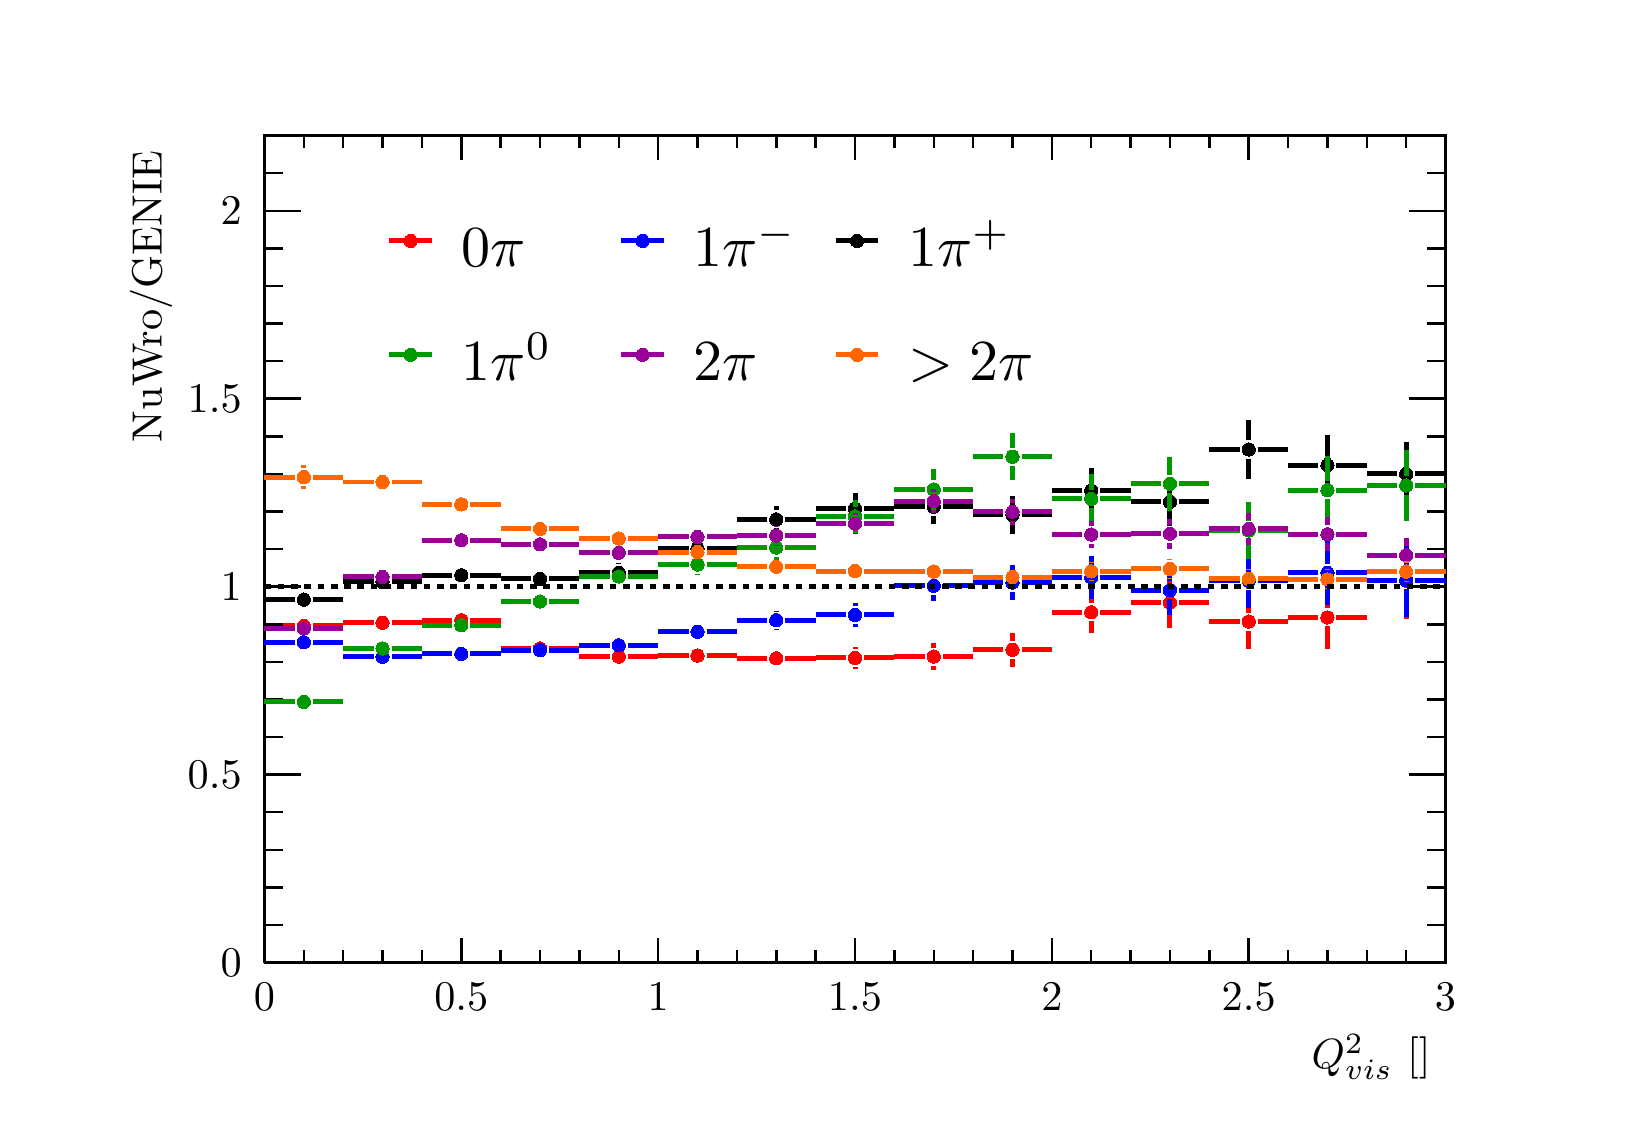
\begin{tikzpicture}
\pgfdeclareplotmark{cross} {
\pgfpathmoveto{\pgfpoint{-0.3\pgfplotmarksize}{\pgfplotmarksize}}
\pgfpathlineto{\pgfpoint{+0.3\pgfplotmarksize}{\pgfplotmarksize}}
\pgfpathlineto{\pgfpoint{+0.3\pgfplotmarksize}{0.3\pgfplotmarksize}}
\pgfpathlineto{\pgfpoint{+1\pgfplotmarksize}{0.3\pgfplotmarksize}}
\pgfpathlineto{\pgfpoint{+1\pgfplotmarksize}{-0.3\pgfplotmarksize}}
\pgfpathlineto{\pgfpoint{+0.3\pgfplotmarksize}{-0.3\pgfplotmarksize}}
\pgfpathlineto{\pgfpoint{+0.3\pgfplotmarksize}{-1.\pgfplotmarksize}}
\pgfpathlineto{\pgfpoint{-0.3\pgfplotmarksize}{-1.\pgfplotmarksize}}
\pgfpathlineto{\pgfpoint{-0.3\pgfplotmarksize}{-0.3\pgfplotmarksize}}
\pgfpathlineto{\pgfpoint{-1.\pgfplotmarksize}{-0.3\pgfplotmarksize}}
\pgfpathlineto{\pgfpoint{-1.\pgfplotmarksize}{0.3\pgfplotmarksize}}
\pgfpathlineto{\pgfpoint{-0.3\pgfplotmarksize}{0.3\pgfplotmarksize}}
\pgfpathclose
\pgfusepathqstroke
}
\pgfdeclareplotmark{cross*} {
\pgfpathmoveto{\pgfpoint{-0.3\pgfplotmarksize}{\pgfplotmarksize}}
\pgfpathlineto{\pgfpoint{+0.3\pgfplotmarksize}{\pgfplotmarksize}}
\pgfpathlineto{\pgfpoint{+0.3\pgfplotmarksize}{0.3\pgfplotmarksize}}
\pgfpathlineto{\pgfpoint{+1\pgfplotmarksize}{0.3\pgfplotmarksize}}
\pgfpathlineto{\pgfpoint{+1\pgfplotmarksize}{-0.3\pgfplotmarksize}}
\pgfpathlineto{\pgfpoint{+0.3\pgfplotmarksize}{-0.3\pgfplotmarksize}}
\pgfpathlineto{\pgfpoint{+0.3\pgfplotmarksize}{-1.\pgfplotmarksize}}
\pgfpathlineto{\pgfpoint{-0.3\pgfplotmarksize}{-1.\pgfplotmarksize}}
\pgfpathlineto{\pgfpoint{-0.3\pgfplotmarksize}{-0.3\pgfplotmarksize}}
\pgfpathlineto{\pgfpoint{-1.\pgfplotmarksize}{-0.3\pgfplotmarksize}}
\pgfpathlineto{\pgfpoint{-1.\pgfplotmarksize}{0.3\pgfplotmarksize}}
\pgfpathlineto{\pgfpoint{-0.3\pgfplotmarksize}{0.3\pgfplotmarksize}}
\pgfpathclose
\pgfusepathqfillstroke
}
\pgfdeclareplotmark{newstar} {
\pgfpathmoveto{\pgfqpoint{0pt}{\pgfplotmarksize}}
\pgfpathlineto{\pgfqpointpolar{44}{0.5\pgfplotmarksize}}
\pgfpathlineto{\pgfqpointpolar{18}{\pgfplotmarksize}}
\pgfpathlineto{\pgfqpointpolar{-20}{0.5\pgfplotmarksize}}
\pgfpathlineto{\pgfqpointpolar{-54}{\pgfplotmarksize}}
\pgfpathlineto{\pgfqpointpolar{-90}{0.5\pgfplotmarksize}}
\pgfpathlineto{\pgfqpointpolar{234}{\pgfplotmarksize}}
\pgfpathlineto{\pgfqpointpolar{198}{0.5\pgfplotmarksize}}
\pgfpathlineto{\pgfqpointpolar{162}{\pgfplotmarksize}}
\pgfpathlineto{\pgfqpointpolar{134}{0.5\pgfplotmarksize}}
\pgfpathclose
\pgfusepathqstroke
}
\pgfdeclareplotmark{newstar*} {
\pgfpathmoveto{\pgfqpoint{0pt}{\pgfplotmarksize}}
\pgfpathlineto{\pgfqpointpolar{44}{0.5\pgfplotmarksize}}
\pgfpathlineto{\pgfqpointpolar{18}{\pgfplotmarksize}}
\pgfpathlineto{\pgfqpointpolar{-20}{0.5\pgfplotmarksize}}
\pgfpathlineto{\pgfqpointpolar{-54}{\pgfplotmarksize}}
\pgfpathlineto{\pgfqpointpolar{-90}{0.5\pgfplotmarksize}}
\pgfpathlineto{\pgfqpointpolar{234}{\pgfplotmarksize}}
\pgfpathlineto{\pgfqpointpolar{198}{0.5\pgfplotmarksize}}
\pgfpathlineto{\pgfqpointpolar{162}{\pgfplotmarksize}}
\pgfpathlineto{\pgfqpointpolar{134}{0.5\pgfplotmarksize}}
\pgfpathclose
\pgfusepathqfillstroke
}
\definecolor{c}{rgb}{1,1,1};
\draw [color=c, fill=c] (0,0) rectangle (20,13.639);
\draw [color=c, fill=c] (3,1.77307) rectangle (18,12.2751);
\definecolor{c}{rgb}{0,0,0};
\draw [c,line width=0.9] (3,1.77307) -- (3,12.2751) -- (18,12.2751) -- (18,1.77307) -- (3,1.77307);
\definecolor{c}{rgb}{1,1,1};
\draw [color=c, fill=c] (3,1.77307) rectangle (18,12.2751);
\definecolor{c}{rgb}{0,0,0};
\draw [c,line width=0.9] (3,1.77307) -- (3,12.2751) -- (18,12.2751) -- (18,1.77307) -- (3,1.77307);
\definecolor{c}{rgb}{1,0,0};
\draw [c,line width=1.8] (3,6.04743) -- (3.38539,6.04743);
\draw [c,line width=1.8] (3.61461,6.04743) -- (4,6.04743);
\foreach \P in {(3.5,6.04743)}{\draw[mark options={color=c,fill=c},mark size=2.402402pt, line width=0.000000pt, mark=*] plot coordinates {\P};}
\draw [c,line width=1.8] (4,6.08852) -- (4.38539,6.08852);
\draw [c,line width=1.8] (4.61461,6.08852) -- (5,6.08852);
\foreach \P in {(4.5,6.08852)}{\draw[mark options={color=c,fill=c},mark size=2.402402pt, line width=0.000000pt, mark=*] plot coordinates {\P};}
\draw [c,line width=1.8] (5,6.12089) -- (5.38539,6.12089);
\draw [c,line width=1.8] (5.61461,6.12089) -- (6,6.12089);
\foreach \P in {(5.5,6.12089)}{\draw[mark options={color=c,fill=c},mark size=2.402402pt, line width=0.000000pt, mark=*] plot coordinates {\P};}
\draw [c,line width=1.8] (6,5.76282) -- (6.38539,5.76282);
\draw [c,line width=1.8] (6.61461,5.76282) -- (7,5.76282);
\foreach \P in {(6.5,5.76282)}{\draw[mark options={color=c,fill=c},mark size=2.402402pt, line width=0.000000pt, mark=*] plot coordinates {\P};}
\draw [c,line width=1.8] (7,5.65759) -- (7.38539,5.65759);
\draw [c,line width=1.8] (7.61461,5.65759) -- (8,5.65759);
\foreach \P in {(7.5,5.65759)}{\draw[mark options={color=c,fill=c},mark size=2.402402pt, line width=0.000000pt, mark=*] plot coordinates {\P};}
\draw [c,line width=1.8] (8,5.6708) -- (8.38539,5.6708);
\draw [c,line width=1.8] (8.61461,5.6708) -- (9,5.6708);
\foreach \P in {(8.5,5.6708)}{\draw[mark options={color=c,fill=c},mark size=2.402402pt, line width=0.000000pt, mark=*] plot coordinates {\P};}
\draw [c,line width=1.8] (9,5.63729) -- (9.38539,5.63729);
\draw [c,line width=1.8] (9.61461,5.63729) -- (10,5.63729);
\foreach \P in {(9.5,5.63729)}{\draw[mark options={color=c,fill=c},mark size=2.402402pt, line width=0.000000pt, mark=*] plot coordinates {\P};}
\draw [c,line width=1.8] (10.5,5.50269) -- (10.5,5.52734);
\draw [c,line width=1.8] (10.5,5.75657) -- (10.5,5.78122);
\draw [c,line width=1.8] (10,5.64196) -- (10.3854,5.64196);
\draw [c,line width=1.8] (10.6146,5.64196) -- (11,5.64196);
\foreach \P in {(10.5,5.64196)}{\draw[mark options={color=c,fill=c},mark size=2.402402pt, line width=0.000000pt, mark=*] plot coordinates {\P};}
\draw [c,line width=1.8] (11.5,5.48713) -- (11.5,5.54456);
\draw [c,line width=1.8] (11.5,5.77379) -- (11.5,5.83122);
\draw [c,line width=1.8] (11,5.65918) -- (11.3854,5.65918);
\draw [c,line width=1.8] (11.6146,5.65918) -- (12,5.65918);
\foreach \P in {(11.5,5.65918)}{\draw[mark options={color=c,fill=c},mark size=2.402402pt, line width=0.000000pt, mark=*] plot coordinates {\P};}
\draw [c,line width=1.8] (12.5,5.53191) -- (12.5,5.63008);
\draw [c,line width=1.8] (12.5,5.8593) -- (12.5,5.95747);
\draw [c,line width=1.8] (12,5.74469) -- (12.3854,5.74469);
\draw [c,line width=1.8] (12.6146,5.74469) -- (13,5.74469);
\foreach \P in {(12.5,5.74469)}{\draw[mark options={color=c,fill=c},mark size=2.402402pt, line width=0.000000pt, mark=*] plot coordinates {\P};}
\draw [c,line width=1.8] (13.5,5.95411) -- (13.5,6.10723);
\draw [c,line width=1.8] (13.5,6.33645) -- (13.5,6.48956);
\draw [c,line width=1.8] (13,6.22184) -- (13.3854,6.22184);
\draw [c,line width=1.8] (13.6146,6.22184) -- (14,6.22184);
\foreach \P in {(13.5,6.22184)}{\draw[mark options={color=c,fill=c},mark size=2.402402pt, line width=0.000000pt, mark=*] plot coordinates {\P};}
\draw [c,line width=1.8] (14.5,6.02788) -- (14.5,6.22779);
\draw [c,line width=1.8] (14.5,6.45701) -- (14.5,6.65692);
\draw [c,line width=1.8] (14,6.3424) -- (14.3854,6.3424);
\draw [c,line width=1.8] (14.6146,6.3424) -- (15,6.3424);
\foreach \P in {(14.5,6.3424)}{\draw[mark options={color=c,fill=c},mark size=2.402402pt, line width=0.000000pt, mark=*] plot coordinates {\P};}
\draw [c,line width=1.8] (15.5,5.75695) -- (15.5,5.98918);
\draw [c,line width=1.8] (15.5,6.21841) -- (15.5,6.45065);
\draw [c,line width=1.8] (15,6.1038) -- (15.3854,6.1038);
\draw [c,line width=1.8] (15.6146,6.1038) -- (16,6.1038);
\foreach \P in {(15.5,6.1038)}{\draw[mark options={color=c,fill=c},mark size=2.402402pt, line width=0.000000pt, mark=*] plot coordinates {\P};}
\draw [c,line width=1.8] (16.5,5.76141) -- (16.5,6.04106);
\draw [c,line width=1.8] (16.5,6.27029) -- (16.5,6.54995);
\draw [c,line width=1.8] (16,6.15568) -- (16.3854,6.15568);
\draw [c,line width=1.8] (16.6146,6.15568) -- (17,6.15568);
\foreach \P in {(16.5,6.15568)}{\draw[mark options={color=c,fill=c},mark size=2.402402pt, line width=0.000000pt, mark=*] plot coordinates {\P};}
\draw [c,line width=1.8] (17.5,6.13333) -- (17.5,6.50904);
\draw [c,line width=1.8] (17.5,6.73827) -- (17.5,7.11399);
\draw [c,line width=1.8] (17,6.62366) -- (17.3854,6.62366);
\draw [c,line width=1.8] (17.6146,6.62366) -- (18,6.62366);
\foreach \P in {(17.5,6.62366)}{\draw[mark options={color=c,fill=c},mark size=2.402402pt, line width=0.000000pt, mark=*] plot coordinates {\P};}
\definecolor{c}{rgb}{0,0,0};
\draw [c,line width=0.9] (3,1.77307) -- (18,1.77307);
\draw [c,line width=0.9] (3,2.07994) -- (3,1.77307);
\draw [c,line width=0.9] (3.5,1.9265) -- (3.5,1.77307);
\draw [c,line width=0.9] (4,1.9265) -- (4,1.77307);
\draw [c,line width=0.9] (4.5,1.9265) -- (4.5,1.77307);
\draw [c,line width=0.9] (5,1.9265) -- (5,1.77307);
\draw [c,line width=0.9] (5.5,2.07994) -- (5.5,1.77307);
\draw [c,line width=0.9] (6,1.9265) -- (6,1.77307);
\draw [c,line width=0.9] (6.5,1.9265) -- (6.5,1.77307);
\draw [c,line width=0.9] (7,1.9265) -- (7,1.77307);
\draw [c,line width=0.9] (7.5,1.9265) -- (7.5,1.77307);
\draw [c,line width=0.9] (8,2.07994) -- (8,1.77307);
\draw [c,line width=0.9] (8.5,1.9265) -- (8.5,1.77307);
\draw [c,line width=0.9] (9,1.9265) -- (9,1.77307);
\draw [c,line width=0.9] (9.5,1.9265) -- (9.5,1.77307);
\draw [c,line width=0.9] (10,1.9265) -- (10,1.77307);
\draw [c,line width=0.9] (10.5,2.07994) -- (10.5,1.77307);
\draw [c,line width=0.9] (11,1.9265) -- (11,1.77307);
\draw [c,line width=0.9] (11.5,1.9265) -- (11.5,1.77307);
\draw [c,line width=0.9] (12,1.9265) -- (12,1.77307);
\draw [c,line width=0.9] (12.5,1.9265) -- (12.5,1.77307);
\draw [c,line width=0.9] (13,2.07994) -- (13,1.77307);
\draw [c,line width=0.9] (13.5,1.9265) -- (13.5,1.77307);
\draw [c,line width=0.9] (14,1.9265) -- (14,1.77307);
\draw [c,line width=0.9] (14.5,1.9265) -- (14.5,1.77307);
\draw [c,line width=0.9] (15,1.9265) -- (15,1.77307);
\draw [c,line width=0.9] (15.5,2.07994) -- (15.5,1.77307);
\draw [c,line width=0.9] (16,1.9265) -- (16,1.77307);
\draw [c,line width=0.9] (16.5,1.9265) -- (16.5,1.77307);
\draw [c,line width=0.9] (17,1.9265) -- (17,1.77307);
\draw [c,line width=0.9] (17.5,1.9265) -- (17.5,1.77307);
\draw [c,line width=0.9] (18,2.07994) -- (18,1.77307);
\draw [c,line width=0.9] (18,2.07994) -- (18,1.77307);
\draw [anchor=base] (3,1.15931) node[scale=1.52731, color=c, rotate=0]{0};
\draw [anchor=base] (5.5,1.15931) node[scale=1.52731, color=c, rotate=0]{0.5};
\draw [anchor=base] (8,1.15931) node[scale=1.52731, color=c, rotate=0]{1};
\draw [anchor=base] (10.5,1.15931) node[scale=1.52731, color=c, rotate=0]{1.5};
\draw [anchor=base] (13,1.15931) node[scale=1.52731, color=c, rotate=0]{2};
\draw [anchor=base] (15.5,1.15931) node[scale=1.52731, color=c, rotate=0]{2.5};
\draw [anchor=base] (18,1.15931) node[scale=1.52731, color=c, rotate=0]{3};
\draw [anchor= east] (18,0.572837) node[scale=1.52731, color=c, rotate=0]{ $Q^{2}_{\text{vis}}$ [\si{\giga\electronvolt\squared}] };
\draw [c,line width=0.9] (3,12.2751) -- (18,12.2751);
\draw [c,line width=0.9] (3,11.9682) -- (3,12.2751);
\draw [c,line width=0.9] (3.5,12.1216) -- (3.5,12.2751);
\draw [c,line width=0.9] (4,12.1216) -- (4,12.2751);
\draw [c,line width=0.9] (4.5,12.1216) -- (4.5,12.2751);
\draw [c,line width=0.9] (5,12.1216) -- (5,12.2751);
\draw [c,line width=0.9] (5.5,11.9682) -- (5.5,12.2751);
\draw [c,line width=0.9] (6,12.1216) -- (6,12.2751);
\draw [c,line width=0.9] (6.5,12.1216) -- (6.5,12.2751);
\draw [c,line width=0.9] (7,12.1216) -- (7,12.2751);
\draw [c,line width=0.9] (7.5,12.1216) -- (7.5,12.2751);
\draw [c,line width=0.9] (8,11.9682) -- (8,12.2751);
\draw [c,line width=0.9] (8.5,12.1216) -- (8.5,12.2751);
\draw [c,line width=0.9] (9,12.1216) -- (9,12.2751);
\draw [c,line width=0.9] (9.5,12.1216) -- (9.5,12.2751);
\draw [c,line width=0.9] (10,12.1216) -- (10,12.2751);
\draw [c,line width=0.9] (10.5,11.9682) -- (10.5,12.2751);
\draw [c,line width=0.9] (11,12.1216) -- (11,12.2751);
\draw [c,line width=0.9] (11.5,12.1216) -- (11.5,12.2751);
\draw [c,line width=0.9] (12,12.1216) -- (12,12.2751);
\draw [c,line width=0.9] (12.5,12.1216) -- (12.5,12.2751);
\draw [c,line width=0.9] (13,11.9682) -- (13,12.2751);
\draw [c,line width=0.9] (13.5,12.1216) -- (13.5,12.2751);
\draw [c,line width=0.9] (14,12.1216) -- (14,12.2751);
\draw [c,line width=0.9] (14.5,12.1216) -- (14.5,12.2751);
\draw [c,line width=0.9] (15,12.1216) -- (15,12.2751);
\draw [c,line width=0.9] (15.5,11.9682) -- (15.5,12.2751);
\draw [c,line width=0.9] (16,12.1216) -- (16,12.2751);
\draw [c,line width=0.9] (16.5,12.1216) -- (16.5,12.2751);
\draw [c,line width=0.9] (17,12.1216) -- (17,12.2751);
\draw [c,line width=0.9] (17.5,12.1216) -- (17.5,12.2751);
\draw [c,line width=0.9] (18,11.9682) -- (18,12.2751);
\draw [c,line width=0.9] (18,11.9682) -- (18,12.2751);
\draw [c,line width=0.9] (3,1.77307) -- (3,12.2751);
\draw [c,line width=0.9] (3.462,1.77307) -- (3,1.77307);
\draw [c,line width=0.9] (3.231,2.25043) -- (3,2.25043);
\draw [c,line width=0.9] (3.231,2.72779) -- (3,2.72779);
\draw [c,line width=0.9] (3.231,3.20516) -- (3,3.20516);
\draw [c,line width=0.9] (3.231,3.68252) -- (3,3.68252);
\draw [c,line width=0.9] (3.462,4.15989) -- (3,4.15989);
\draw [c,line width=0.9] (3.231,4.63725) -- (3,4.63725);
\draw [c,line width=0.9] (3.231,5.11461) -- (3,5.11461);
\draw [c,line width=0.9] (3.231,5.59198) -- (3,5.59198);
\draw [c,line width=0.9] (3.231,6.06934) -- (3,6.06934);
\draw [c,line width=0.9] (3.462,6.5467) -- (3,6.5467);
\draw [c,line width=0.9] (3.231,7.02407) -- (3,7.02407);
\draw [c,line width=0.9] (3.231,7.50143) -- (3,7.50143);
\draw [c,line width=0.9] (3.231,7.9788) -- (3,7.9788);
\draw [c,line width=0.9] (3.231,8.45616) -- (3,8.45616);
\draw [c,line width=0.9] (3.462,8.93352) -- (3,8.93352);
\draw [c,line width=0.9] (3.231,9.41089) -- (3,9.41089);
\draw [c,line width=0.9] (3.231,9.88825) -- (3,9.88825);
\draw [c,line width=0.9] (3.231,10.3656) -- (3,10.3656);
\draw [c,line width=0.9] (3.231,10.843) -- (3,10.843);
\draw [c,line width=0.9] (3.462,11.3203) -- (3,11.3203);
\draw [c,line width=0.9] (3.462,11.3203) -- (3,11.3203);
\draw [c,line width=0.9] (3.231,11.7977) -- (3,11.7977);
\draw [c,line width=0.9] (3.231,12.2751) -- (3,12.2751);
\draw [anchor= east] (2.9,1.77307) node[scale=1.52731, color=c, rotate=0]{0};
\draw [anchor= east] (2.9,4.15989) node[scale=1.52731, color=c, rotate=0]{0.5};
\draw [anchor= east] (2.9,6.5467) node[scale=1.52731, color=c, rotate=0]{1};
\draw [anchor= east] (2.9,8.93352) node[scale=1.52731, color=c, rotate=0]{1.5};
\draw [anchor= east] (2.9,11.3203) node[scale=1.52731, color=c, rotate=0]{2};
\draw [anchor= east] (1.56,12.2751) node[scale=1.52731, color=c, rotate=90]{ NuWro/GENIE};
\draw [c,line width=0.9] (18,1.77307) -- (18,12.2751);
\draw [c,line width=0.9] (17.538,1.77307) -- (18,1.77307);
\draw [c,line width=0.9] (17.769,2.25043) -- (18,2.25043);
\draw [c,line width=0.9] (17.769,2.72779) -- (18,2.72779);
\draw [c,line width=0.9] (17.769,3.20516) -- (18,3.20516);
\draw [c,line width=0.9] (17.769,3.68252) -- (18,3.68252);
\draw [c,line width=0.9] (17.538,4.15989) -- (18,4.15989);
\draw [c,line width=0.9] (17.769,4.63725) -- (18,4.63725);
\draw [c,line width=0.9] (17.769,5.11461) -- (18,5.11461);
\draw [c,line width=0.9] (17.769,5.59198) -- (18,5.59198);
\draw [c,line width=0.9] (17.769,6.06934) -- (18,6.06934);
\draw [c,line width=0.9] (17.538,6.5467) -- (18,6.5467);
\draw [c,line width=0.9] (17.769,7.02407) -- (18,7.02407);
\draw [c,line width=0.9] (17.769,7.50143) -- (18,7.50143);
\draw [c,line width=0.9] (17.769,7.9788) -- (18,7.9788);
\draw [c,line width=0.9] (17.769,8.45616) -- (18,8.45616);
\draw [c,line width=0.9] (17.538,8.93352) -- (18,8.93352);
\draw [c,line width=0.9] (17.769,9.41089) -- (18,9.41089);
\draw [c,line width=0.9] (17.769,9.88825) -- (18,9.88825);
\draw [c,line width=0.9] (17.769,10.3656) -- (18,10.3656);
\draw [c,line width=0.9] (17.769,10.843) -- (18,10.843);
\draw [c,line width=0.9] (17.538,11.3203) -- (18,11.3203);
\draw [c,line width=0.9] (17.538,11.3203) -- (18,11.3203);
\draw [c,line width=0.9] (17.769,11.7977) -- (18,11.7977);
\draw [c,line width=0.9] (17.769,12.2751) -- (18,12.2751);
\definecolor{c}{rgb}{0,0,1};
\draw [c,line width=1.8] (3,5.8411) -- (3.38539,5.8411);
\draw [c,line width=1.8] (3.61461,5.8411) -- (4,5.8411);
\foreach \P in {(3.5,5.8411)}{\draw[mark options={color=c,fill=c},mark size=2.402402pt, line width=0.000000pt, mark=*] plot coordinates {\P};}
\draw [c,line width=1.8] (4,5.65657) -- (4.38539,5.65657);
\draw [c,line width=1.8] (4.61461,5.65657) -- (5,5.65657);
\foreach \P in {(4.5,5.65657)}{\draw[mark options={color=c,fill=c},mark size=2.402402pt, line width=0.000000pt, mark=*] plot coordinates {\P};}
\draw [c,line width=1.8] (5,5.69388) -- (5.38539,5.69388);
\draw [c,line width=1.8] (5.61461,5.69388) -- (6,5.69388);
\foreach \P in {(5.5,5.69388)}{\draw[mark options={color=c,fill=c},mark size=2.402402pt, line width=0.000000pt, mark=*] plot coordinates {\P};}
\draw [c,line width=1.8] (6,5.74041) -- (6.38539,5.74041);
\draw [c,line width=1.8] (6.61461,5.74041) -- (7,5.74041);
\foreach \P in {(6.5,5.74041)}{\draw[mark options={color=c,fill=c},mark size=2.402402pt, line width=0.000000pt, mark=*] plot coordinates {\P};}
\draw [c,line width=1.8] (7,5.80259) -- (7.38539,5.80259);
\draw [c,line width=1.8] (7.61461,5.80259) -- (8,5.80259);
\foreach \P in {(7.5,5.80259)}{\draw[mark options={color=c,fill=c},mark size=2.402402pt, line width=0.000000pt, mark=*] plot coordinates {\P};}
\draw [c,line width=1.8] (8,5.97399) -- (8.38539,5.97399);
\draw [c,line width=1.8] (8.61461,5.97399) -- (9,5.97399);
\foreach \P in {(8.5,5.97399)}{\draw[mark options={color=c,fill=c},mark size=2.402402pt, line width=0.000000pt, mark=*] plot coordinates {\P};}
\draw [c,line width=1.8] (9.5,5.99969) -- (9.5,6.00656);
\draw [c,line width=1.8] (9.5,6.23578) -- (9.5,6.24265);
\draw [c,line width=1.8] (9,6.12117) -- (9.38539,6.12117);
\draw [c,line width=1.8] (9.61461,6.12117) -- (10,6.12117);
\foreach \P in {(9.5,6.12117)}{\draw[mark options={color=c,fill=c},mark size=2.402402pt, line width=0.000000pt, mark=*] plot coordinates {\P};}
\draw [c,line width=1.8] (10.5,6.0396) -- (10.5,6.07429);
\draw [c,line width=1.8] (10.5,6.30352) -- (10.5,6.3382);
\draw [c,line width=1.8] (10,6.1889) -- (10.3854,6.1889);
\draw [c,line width=1.8] (10.6146,6.1889) -- (11,6.1889);
\foreach \P in {(10.5,6.1889)}{\draw[mark options={color=c,fill=c},mark size=2.402402pt, line width=0.000000pt, mark=*] plot coordinates {\P};}
\draw [c,line width=1.8] (11.5,6.36671) -- (11.5,6.44376);
\draw [c,line width=1.8] (11.5,6.67299) -- (11.5,6.75003);
\draw [c,line width=1.8] (11,6.55837) -- (11.3854,6.55837);
\draw [c,line width=1.8] (11.6146,6.55837) -- (12,6.55837);
\foreach \P in {(11.5,6.55837)}{\draw[mark options={color=c,fill=c},mark size=2.402402pt, line width=0.000000pt, mark=*] plot coordinates {\P};}
\draw [c,line width=1.8] (12.5,6.3725) -- (12.5,6.48521);
\draw [c,line width=1.8] (12.5,6.71443) -- (12.5,6.82713);
\draw [c,line width=1.8] (12,6.59982) -- (12.3854,6.59982);
\draw [c,line width=1.8] (12.6146,6.59982) -- (13,6.59982);
\foreach \P in {(12.5,6.59982)}{\draw[mark options={color=c,fill=c},mark size=2.402402pt, line width=0.000000pt, mark=*] plot coordinates {\P};}
\draw [c,line width=1.8] (13.5,6.39344) -- (13.5,6.5512);
\draw [c,line width=1.8] (13.5,6.78043) -- (13.5,6.93819);
\draw [c,line width=1.8] (13,6.66581) -- (13.3854,6.66581);
\draw [c,line width=1.8] (13.6146,6.66581) -- (14,6.66581);
\foreach \P in {(13.5,6.66581)}{\draw[mark options={color=c,fill=c},mark size=2.402402pt, line width=0.000000pt, mark=*] plot coordinates {\P};}
\draw [c,line width=1.8] (14.5,6.19266) -- (14.5,6.38715);
\draw [c,line width=1.8] (14.5,6.61638) -- (14.5,6.81087);
\draw [c,line width=1.8] (14,6.50176) -- (14.3854,6.50176);
\draw [c,line width=1.8] (14.6146,6.50176) -- (15,6.50176);
\foreach \P in {(14.5,6.50176)}{\draw[mark options={color=c,fill=c},mark size=2.402402pt, line width=0.000000pt, mark=*] plot coordinates {\P};}
\draw [c,line width=1.8] (15.5,6.27302) -- (15.5,6.50785);
\draw [c,line width=1.8] (15.5,6.73708) -- (15.5,6.9719);
\draw [c,line width=1.8] (15,6.62246) -- (15.3854,6.62246);
\draw [c,line width=1.8] (15.6146,6.62246) -- (16,6.62246);
\foreach \P in {(15.5,6.62246)}{\draw[mark options={color=c,fill=c},mark size=2.402402pt, line width=0.000000pt, mark=*] plot coordinates {\P};}
\draw [c,line width=1.8] (16.5,6.30891) -- (16.5,6.60758);
\draw [c,line width=1.8] (16.5,6.83681) -- (16.5,7.13549);
\draw [c,line width=1.8] (16,6.7222) -- (16.3854,6.7222);
\draw [c,line width=1.8] (16.6146,6.7222) -- (17,6.7222);
\foreach \P in {(16.5,6.7222)}{\draw[mark options={color=c,fill=c},mark size=2.402402pt, line width=0.000000pt, mark=*] plot coordinates {\P};}
\draw [c,line width=1.8] (17.5,6.16306) -- (17.5,6.51295);
\draw [c,line width=1.8] (17.5,6.74218) -- (17.5,7.09208);
\draw [c,line width=1.8] (17,6.62757) -- (17.3854,6.62757);
\draw [c,line width=1.8] (17.6146,6.62757) -- (18,6.62757);
\foreach \P in {(17.5,6.62757)}{\draw[mark options={color=c,fill=c},mark size=2.402402pt, line width=0.000000pt, mark=*] plot coordinates {\P};}
\definecolor{c}{rgb}{0,0,0};
\draw [c,line width=1.8] (3,6.38243) -- (3.38539,6.38243);
\draw [c,line width=1.8] (3.61461,6.38243) -- (4,6.38243);
\foreach \P in {(3.5,6.38243)}{\draw[mark options={color=c,fill=c},mark size=2.402402pt, line width=0.000000pt, mark=*] plot coordinates {\P};}
\draw [c,line width=1.8] (4,6.60756) -- (4.38539,6.60756);
\draw [c,line width=1.8] (4.61461,6.60756) -- (5,6.60756);
\foreach \P in {(4.5,6.60756)}{\draw[mark options={color=c,fill=c},mark size=2.402402pt, line width=0.000000pt, mark=*] plot coordinates {\P};}
\draw [c,line width=1.8] (5,6.69119) -- (5.38539,6.69119);
\draw [c,line width=1.8] (5.61461,6.69119) -- (6,6.69119);
\foreach \P in {(5.5,6.69119)}{\draw[mark options={color=c,fill=c},mark size=2.402402pt, line width=0.000000pt, mark=*] plot coordinates {\P};}
\draw [c,line width=1.8] (6,6.64474) -- (6.38539,6.64474);
\draw [c,line width=1.8] (6.61461,6.64474) -- (7,6.64474);
\foreach \P in {(6.5,6.64474)}{\draw[mark options={color=c,fill=c},mark size=2.402402pt, line width=0.000000pt, mark=*] plot coordinates {\P};}
\draw [c,line width=1.8] (7.5,6.60047) -- (7.5,6.60934);
\draw [c,line width=1.8] (7.5,6.83857) -- (7.5,6.84744);
\draw [c,line width=1.8] (7,6.72395) -- (7.38539,6.72395);
\draw [c,line width=1.8] (7.61461,6.72395) -- (8,6.72395);
\foreach \P in {(7.5,6.72395)}{\draw[mark options={color=c,fill=c},mark size=2.402402pt, line width=0.000000pt, mark=*] plot coordinates {\P};}
\draw [c,line width=1.8] (8.5,6.88555) -- (8.5,6.91554);
\draw [c,line width=1.8] (8.5,7.14476) -- (8.5,7.17475);
\draw [c,line width=1.8] (8,7.03015) -- (8.38539,7.03015);
\draw [c,line width=1.8] (8.61461,7.03015) -- (9,7.03015);
\foreach \P in {(8.5,7.03015)}{\draw[mark options={color=c,fill=c},mark size=2.402402pt, line width=0.000000pt, mark=*] plot coordinates {\P};}
\draw [c,line width=1.8] (9.5,7.23195) -- (9.5,7.28672);
\draw [c,line width=1.8] (9.5,7.51594) -- (9.5,7.57072);
\draw [c,line width=1.8] (9,7.40133) -- (9.38539,7.40133);
\draw [c,line width=1.8] (9.61461,7.40133) -- (10,7.40133);
\foreach \P in {(9.5,7.40133)}{\draw[mark options={color=c,fill=c},mark size=2.402402pt, line width=0.000000pt, mark=*] plot coordinates {\P};}
\draw [c,line width=1.8] (10.5,7.33699) -- (10.5,7.42229);
\draw [c,line width=1.8] (10.5,7.65151) -- (10.5,7.73682);
\draw [c,line width=1.8] (10,7.5369) -- (10.3854,7.5369);
\draw [c,line width=1.8] (10.6146,7.5369) -- (11,7.5369);
\foreach \P in {(10.5,7.5369)}{\draw[mark options={color=c,fill=c},mark size=2.402402pt, line width=0.000000pt, mark=*] plot coordinates {\P};}
\draw [c,line width=1.8] (11.5,7.33972) -- (11.5,7.44719);
\draw [c,line width=1.8] (11.5,7.67642) -- (11.5,7.78389);
\draw [c,line width=1.8] (11,7.5618) -- (11.3854,7.5618);
\draw [c,line width=1.8] (11.6146,7.5618) -- (12,7.5618);
\foreach \P in {(11.5,7.5618)}{\draw[mark options={color=c,fill=c},mark size=2.402402pt, line width=0.000000pt, mark=*] plot coordinates {\P};}
\draw [c,line width=1.8] (12.5,7.21433) -- (12.5,7.34363);
\draw [c,line width=1.8] (12.5,7.57285) -- (12.5,7.70215);
\draw [c,line width=1.8] (12,7.45824) -- (12.3854,7.45824);
\draw [c,line width=1.8] (12.6146,7.45824) -- (13,7.45824);
\foreach \P in {(12.5,7.45824)}{\draw[mark options={color=c,fill=c},mark size=2.402402pt, line width=0.000000pt, mark=*] plot coordinates {\P};}
\draw [c,line width=1.8] (13.5,7.48431) -- (13.5,7.6524);
\draw [c,line width=1.8] (13.5,7.88163) -- (13.5,8.04972);
\draw [c,line width=1.8] (13,7.76701) -- (13.3854,7.76701);
\draw [c,line width=1.8] (13.6146,7.76701) -- (14,7.76701);
\foreach \P in {(13.5,7.76701)}{\draw[mark options={color=c,fill=c},mark size=2.402402pt, line width=0.000000pt, mark=*] plot coordinates {\P};}
\draw [c,line width=1.8] (14.5,7.31124) -- (14.5,7.50959);
\draw [c,line width=1.8] (14.5,7.73882) -- (14.5,7.93717);
\draw [c,line width=1.8] (14,7.62421) -- (14.3854,7.62421);
\draw [c,line width=1.8] (14.6146,7.62421) -- (15,7.62421);
\foreach \P in {(14.5,7.62421)}{\draw[mark options={color=c,fill=c},mark size=2.402402pt, line width=0.000000pt, mark=*] plot coordinates {\P};}
\draw [c,line width=1.8] (15.5,7.91638) -- (15.5,8.17441);
\draw [c,line width=1.8] (15.5,8.40363) -- (15.5,8.66166);
\draw [c,line width=1.8] (15,8.28902) -- (15.3854,8.28902);
\draw [c,line width=1.8] (15.6146,8.28902) -- (16,8.28902);
\foreach \P in {(15.5,8.28902)}{\draw[mark options={color=c,fill=c},mark size=2.402402pt, line width=0.000000pt, mark=*] plot coordinates {\P};}
\draw [c,line width=1.8] (16.5,7.70917) -- (16.5,7.97604);
\draw [c,line width=1.8] (16.5,8.20526) -- (16.5,8.47213);
\draw [c,line width=1.8] (16,8.09065) -- (16.3854,8.09065);
\draw [c,line width=1.8] (16.6146,8.09065) -- (17,8.09065);
\foreach \P in {(16.5,8.09065)}{\draw[mark options={color=c,fill=c},mark size=2.402402pt, line width=0.000000pt, mark=*] plot coordinates {\P};}
\draw [c,line width=1.8] (17.5,7.57129) -- (17.5,7.86363);
\draw [c,line width=1.8] (17.5,8.09286) -- (17.5,8.3852);
\draw [c,line width=1.8] (17,7.97824) -- (17.3854,7.97824);
\draw [c,line width=1.8] (17.6146,7.97824) -- (18,7.97824);
\foreach \P in {(17.5,7.97824)}{\draw[mark options={color=c,fill=c},mark size=2.402402pt, line width=0.000000pt, mark=*] plot coordinates {\P};}
\definecolor{c}{rgb}{0,0.6,0};
\draw [c,line width=1.8] (3,5.0845) -- (3.38539,5.0845);
\draw [c,line width=1.8] (3.61461,5.0845) -- (4,5.0845);
\foreach \P in {(3.5,5.0845)}{\draw[mark options={color=c,fill=c},mark size=2.402402pt, line width=0.000000pt, mark=*] plot coordinates {\P};}
\draw [c,line width=1.8] (4,5.76187) -- (4.38539,5.76187);
\draw [c,line width=1.8] (4.61461,5.76187) -- (5,5.76187);
\foreach \P in {(4.5,5.76187)}{\draw[mark options={color=c,fill=c},mark size=2.402402pt, line width=0.000000pt, mark=*] plot coordinates {\P};}
\draw [c,line width=1.8] (5,6.05624) -- (5.38539,6.05624);
\draw [c,line width=1.8] (5.61461,6.05624) -- (6,6.05624);
\foreach \P in {(5.5,6.05624)}{\draw[mark options={color=c,fill=c},mark size=2.402402pt, line width=0.000000pt, mark=*] plot coordinates {\P};}
\draw [c,line width=1.8] (6,6.35791) -- (6.38539,6.35791);
\draw [c,line width=1.8] (6.61461,6.35791) -- (7,6.35791);
\foreach \P in {(6.5,6.35791)}{\draw[mark options={color=c,fill=c},mark size=2.402402pt, line width=0.000000pt, mark=*] plot coordinates {\P};}
\draw [c,line width=1.8] (7,6.67594) -- (7.38539,6.67594);
\draw [c,line width=1.8] (7.61461,6.67594) -- (8,6.67594);
\foreach \P in {(7.5,6.67594)}{\draw[mark options={color=c,fill=c},mark size=2.402402pt, line width=0.000000pt, mark=*] plot coordinates {\P};}
\draw [c,line width=1.8] (8.5,6.68893) -- (8.5,6.71382);
\draw [c,line width=1.8] (8.5,6.94304) -- (8.5,6.96793);
\draw [c,line width=1.8] (8,6.82843) -- (8.38539,6.82843);
\draw [c,line width=1.8] (8.61461,6.82843) -- (9,6.82843);
\foreach \P in {(8.5,6.82843)}{\draw[mark options={color=c,fill=c},mark size=2.402402pt, line width=0.000000pt, mark=*] plot coordinates {\P};}
\draw [c,line width=1.8] (9.5,6.87207) -- (9.5,6.92823);
\draw [c,line width=1.8] (9.5,7.15746) -- (9.5,7.21361);
\draw [c,line width=1.8] (9,7.04284) -- (9.38539,7.04284);
\draw [c,line width=1.8] (9.61461,7.04284) -- (10,7.04284);
\foreach \P in {(9.5,7.04284)}{\draw[mark options={color=c,fill=c},mark size=2.402402pt, line width=0.000000pt, mark=*] plot coordinates {\P};}
\draw [c,line width=1.8] (10.5,7.22658) -- (10.5,7.32438);
\draw [c,line width=1.8] (10.5,7.55361) -- (10.5,7.65141);
\draw [c,line width=1.8] (10,7.439) -- (10.3854,7.439);
\draw [c,line width=1.8] (10.6146,7.439) -- (11,7.439);
\foreach \P in {(10.5,7.439)}{\draw[mark options={color=c,fill=c},mark size=2.402402pt, line width=0.000000pt, mark=*] plot coordinates {\P};}
\draw [c,line width=1.8] (11.5,7.52671) -- (11.5,7.66743);
\draw [c,line width=1.8] (11.5,7.89666) -- (11.5,8.03737);
\draw [c,line width=1.8] (11,7.78204) -- (11.3854,7.78204);
\draw [c,line width=1.8] (11.6146,7.78204) -- (12,7.78204);
\foreach \P in {(11.5,7.78204)}{\draw[mark options={color=c,fill=c},mark size=2.402402pt, line width=0.000000pt, mark=*] plot coordinates {\P};}
\draw [c,line width=1.8] (12.5,7.89831) -- (12.5,8.08322);
\draw [c,line width=1.8] (12.5,8.31245) -- (12.5,8.49736);
\draw [c,line width=1.8] (12,8.19783) -- (12.3854,8.19783);
\draw [c,line width=1.8] (12.6146,8.19783) -- (13,8.19783);
\foreach \P in {(12.5,8.19783)}{\draw[mark options={color=c,fill=c},mark size=2.402402pt, line width=0.000000pt, mark=*] plot coordinates {\P};}
\draw [c,line width=1.8] (13.5,7.34692) -- (13.5,7.54667);
\draw [c,line width=1.8] (13.5,7.7759) -- (13.5,7.97565);
\draw [c,line width=1.8] (13,7.66128) -- (13.3854,7.66128);
\draw [c,line width=1.8] (13.6146,7.66128) -- (14,7.66128);
\foreach \P in {(13.5,7.66128)}{\draw[mark options={color=c,fill=c},mark size=2.402402pt, line width=0.000000pt, mark=*] plot coordinates {\P};}
\draw [c,line width=1.8] (14.5,7.51028) -- (14.5,7.73894);
\draw [c,line width=1.8] (14.5,7.96817) -- (14.5,8.19684);
\draw [c,line width=1.8] (14,7.85356) -- (14.3854,7.85356);
\draw [c,line width=1.8] (14.6146,7.85356) -- (15,7.85356);
\foreach \P in {(14.5,7.85356)}{\draw[mark options={color=c,fill=c},mark size=2.402402pt, line width=0.000000pt, mark=*] plot coordinates {\P};}
\draw [c,line width=1.8] (15.5,6.89466) -- (15.5,7.14606);
\draw [c,line width=1.8] (15.5,7.37529) -- (15.5,7.62669);
\draw [c,line width=1.8] (15,7.26068) -- (15.3854,7.26068);
\draw [c,line width=1.8] (15.6146,7.26068) -- (16,7.26068);
\foreach \P in {(15.5,7.26068)}{\draw[mark options={color=c,fill=c},mark size=2.402402pt, line width=0.000000pt, mark=*] plot coordinates {\P};}
\draw [c,line width=1.8] (16.5,7.34328) -- (16.5,7.65794);
\draw [c,line width=1.8] (16.5,7.88716) -- (16.5,8.20182);
\draw [c,line width=1.8] (16,7.77255) -- (16.3854,7.77255);
\draw [c,line width=1.8] (16.6146,7.77255) -- (17,7.77255);
\foreach \P in {(16.5,7.77255)}{\draw[mark options={color=c,fill=c},mark size=2.402402pt, line width=0.000000pt, mark=*] plot coordinates {\P};}
\draw [c,line width=1.8] (17.5,7.37887) -- (17.5,7.71679);
\draw [c,line width=1.8] (17.5,7.94602) -- (17.5,8.28395);
\draw [c,line width=1.8] (17,7.83141) -- (17.3854,7.83141);
\draw [c,line width=1.8] (17.6146,7.83141) -- (18,7.83141);
\foreach \P in {(17.5,7.83141)}{\draw[mark options={color=c,fill=c},mark size=2.402402pt, line width=0.000000pt, mark=*] plot coordinates {\P};}
\definecolor{c}{rgb}{0.6,0,0.6};
\draw [c,line width=1.8] (3,6.01773) -- (3.38539,6.01773);
\draw [c,line width=1.8] (3.61461,6.01773) -- (4,6.01773);
\foreach \P in {(3.5,6.01773)}{\draw[mark options={color=c,fill=c},mark size=2.402402pt, line width=0.000000pt, mark=*] plot coordinates {\P};}
\draw [c,line width=1.8] (4,6.67018) -- (4.38539,6.67018);
\draw [c,line width=1.8] (4.61461,6.67018) -- (5,6.67018);
\foreach \P in {(4.5,6.67018)}{\draw[mark options={color=c,fill=c},mark size=2.402402pt, line width=0.000000pt, mark=*] plot coordinates {\P};}
\draw [c,line width=1.8] (5,7.13666) -- (5.38539,7.13666);
\draw [c,line width=1.8] (5.61461,7.13666) -- (6,7.13666);
\foreach \P in {(5.5,7.13666)}{\draw[mark options={color=c,fill=c},mark size=2.402402pt, line width=0.000000pt, mark=*] plot coordinates {\P};}
\draw [c,line width=1.8] (6,7.08508) -- (6.38539,7.08508);
\draw [c,line width=1.8] (6.61461,7.08508) -- (7,7.08508);
\foreach \P in {(6.5,7.08508)}{\draw[mark options={color=c,fill=c},mark size=2.402402pt, line width=0.000000pt, mark=*] plot coordinates {\P};}
\draw [c,line width=1.8] (7,6.97753) -- (7.38539,6.97753);
\draw [c,line width=1.8] (7.61461,6.97753) -- (8,6.97753);
\foreach \P in {(7.5,6.97753)}{\draw[mark options={color=c,fill=c},mark size=2.402402pt, line width=0.000000pt, mark=*] plot coordinates {\P};}
\draw [c,line width=1.8] (8,7.17875) -- (8.38539,7.17875);
\draw [c,line width=1.8] (8.61461,7.17875) -- (9,7.17875);
\foreach \P in {(8.5,7.17875)}{\draw[mark options={color=c,fill=c},mark size=2.402402pt, line width=0.000000pt, mark=*] plot coordinates {\P};}
\draw [c,line width=1.8] (9.5,7.07924) -- (9.5,7.08128);
\draw [c,line width=1.8] (9.5,7.3105) -- (9.5,7.31254);
\draw [c,line width=1.8] (9,7.19589) -- (9.38539,7.19589);
\draw [c,line width=1.8] (9.61461,7.19589) -- (10,7.19589);
\foreach \P in {(9.5,7.19589)}{\draw[mark options={color=c,fill=c},mark size=2.402402pt, line width=0.000000pt, mark=*] plot coordinates {\P};}
\draw [c,line width=1.8] (10.5,7.21138) -- (10.5,7.23198);
\draw [c,line width=1.8] (10.5,7.46121) -- (10.5,7.48181);
\draw [c,line width=1.8] (10,7.34659) -- (10.3854,7.34659);
\draw [c,line width=1.8] (10.6146,7.34659) -- (11,7.34659);
\foreach \P in {(10.5,7.34659)}{\draw[mark options={color=c,fill=c},mark size=2.402402pt, line width=0.000000pt, mark=*] plot coordinates {\P};}
\draw [c,line width=1.8] (11.5,7.48113) -- (11.5,7.51879);
\draw [c,line width=1.8] (11.5,7.74801) -- (11.5,7.78568);
\draw [c,line width=1.8] (11,7.6334) -- (11.3854,7.6334);
\draw [c,line width=1.8] (11.6146,7.6334) -- (12,7.6334);
\foreach \P in {(11.5,7.6334)}{\draw[mark options={color=c,fill=c},mark size=2.402402pt, line width=0.000000pt, mark=*] plot coordinates {\P};}
\draw [c,line width=1.8] (12.5,7.33162) -- (12.5,7.38234);
\draw [c,line width=1.8] (12.5,7.61157) -- (12.5,7.66228);
\draw [c,line width=1.8] (12,7.49695) -- (12.3854,7.49695);
\draw [c,line width=1.8] (12.6146,7.49695) -- (13,7.49695);
\foreach \P in {(12.5,7.49695)}{\draw[mark options={color=c,fill=c},mark size=2.402402pt, line width=0.000000pt, mark=*] plot coordinates {\P};}
\draw [c,line width=1.8] (13.5,7.03552) -- (13.5,7.09412);
\draw [c,line width=1.8] (13.5,7.32335) -- (13.5,7.38194);
\draw [c,line width=1.8] (13,7.20873) -- (13.3854,7.20873);
\draw [c,line width=1.8] (13.6146,7.20873) -- (14,7.20873);
\foreach \P in {(13.5,7.20873)}{\draw[mark options={color=c,fill=c},mark size=2.402402pt, line width=0.000000pt, mark=*] plot coordinates {\P};}
\draw [c,line width=1.8] (14.5,7.02919) -- (14.5,7.10444);
\draw [c,line width=1.8] (14.5,7.33367) -- (14.5,7.40893);
\draw [c,line width=1.8] (14,7.21906) -- (14.3854,7.21906);
\draw [c,line width=1.8] (14.6146,7.21906) -- (15,7.21906);
\foreach \P in {(14.5,7.21906)}{\draw[mark options={color=c,fill=c},mark size=2.402402pt, line width=0.000000pt, mark=*] plot coordinates {\P};}
\draw [c,line width=1.8] (15.5,7.07526) -- (15.5,7.16585);
\draw [c,line width=1.8] (15.5,7.39508) -- (15.5,7.48567);
\draw [c,line width=1.8] (15,7.28047) -- (15.3854,7.28047);
\draw [c,line width=1.8] (15.6146,7.28047) -- (16,7.28047);
\foreach \P in {(15.5,7.28047)}{\draw[mark options={color=c,fill=c},mark size=2.402402pt, line width=0.000000pt, mark=*] plot coordinates {\P};}
\draw [c,line width=1.8] (16.5,6.99694) -- (16.5,7.09698);
\draw [c,line width=1.8] (16.5,7.3262) -- (16.5,7.42624);
\draw [c,line width=1.8] (16,7.21159) -- (16.3854,7.21159);
\draw [c,line width=1.8] (16.6146,7.21159) -- (17,7.21159);
\foreach \P in {(16.5,7.21159)}{\draw[mark options={color=c,fill=c},mark size=2.402402pt, line width=0.000000pt, mark=*] plot coordinates {\P};}
\draw [c,line width=1.8] (17.5,6.72299) -- (17.5,6.83154);
\draw [c,line width=1.8] (17.5,7.06077) -- (17.5,7.16932);
\draw [c,line width=1.8] (17,6.94615) -- (17.3854,6.94615);
\draw [c,line width=1.8] (17.6146,6.94615) -- (18,6.94615);
\foreach \P in {(17.5,6.94615)}{\draw[mark options={color=c,fill=c},mark size=2.402402pt, line width=0.000000pt, mark=*] plot coordinates {\P};}
\definecolor{c}{rgb}{1,0.4,0};
\draw [c,line width=1.8] (3.5,7.78749) -- (3.5,7.82423);
\draw [c,line width=1.8] (3.5,8.05345) -- (3.5,8.09019);
\draw [c,line width=1.8] (3,7.93884) -- (3.38539,7.93884);
\draw [c,line width=1.8] (3.61461,7.93884) -- (4,7.93884);
\foreach \P in {(3.5,7.93884)}{\draw[mark options={color=c,fill=c},mark size=2.402402pt, line width=0.000000pt, mark=*] plot coordinates {\P};}
\draw [c,line width=1.8] (4,7.87607) -- (4.38539,7.87607);
\draw [c,line width=1.8] (4.61461,7.87607) -- (5,7.87607);
\foreach \P in {(4.5,7.87607)}{\draw[mark options={color=c,fill=c},mark size=2.402402pt, line width=0.000000pt, mark=*] plot coordinates {\P};}
\draw [c,line width=1.8] (5,7.59204) -- (5.38539,7.59204);
\draw [c,line width=1.8] (5.61461,7.59204) -- (6,7.59204);
\foreach \P in {(5.5,7.59204)}{\draw[mark options={color=c,fill=c},mark size=2.402402pt, line width=0.000000pt, mark=*] plot coordinates {\P};}
\draw [c,line width=1.8] (6,7.28163) -- (6.38539,7.28163);
\draw [c,line width=1.8] (6.61461,7.28163) -- (7,7.28163);
\foreach \P in {(6.5,7.28163)}{\draw[mark options={color=c,fill=c},mark size=2.402402pt, line width=0.000000pt, mark=*] plot coordinates {\P};}
\draw [c,line width=1.8] (7,7.15891) -- (7.38539,7.15891);
\draw [c,line width=1.8] (7.61461,7.15891) -- (8,7.15891);
\foreach \P in {(7.5,7.15891)}{\draw[mark options={color=c,fill=c},mark size=2.402402pt, line width=0.000000pt, mark=*] plot coordinates {\P};}
\draw [c,line width=1.8] (8,6.98676) -- (8.38539,6.98676);
\draw [c,line width=1.8] (8.61461,6.98676) -- (9,6.98676);
\foreach \P in {(8.5,6.98676)}{\draw[mark options={color=c,fill=c},mark size=2.402402pt, line width=0.000000pt, mark=*] plot coordinates {\P};}
\draw [c,line width=1.8] (9,6.7994) -- (9.38539,6.7994);
\draw [c,line width=1.8] (9.61461,6.7994) -- (10,6.7994);
\foreach \P in {(9.5,6.7994)}{\draw[mark options={color=c,fill=c},mark size=2.402402pt, line width=0.000000pt, mark=*] plot coordinates {\P};}
\draw [c,line width=1.8] (10,6.74503) -- (10.3854,6.74503);
\draw [c,line width=1.8] (10.6146,6.74503) -- (11,6.74503);
\foreach \P in {(10.5,6.74503)}{\draw[mark options={color=c,fill=c},mark size=2.402402pt, line width=0.000000pt, mark=*] plot coordinates {\P};}
\draw [c,line width=1.8] (11,6.73919) -- (11.3854,6.73919);
\draw [c,line width=1.8] (11.6146,6.73919) -- (12,6.73919);
\foreach \P in {(11.5,6.73919)}{\draw[mark options={color=c,fill=c},mark size=2.402402pt, line width=0.000000pt, mark=*] plot coordinates {\P};}
\draw [c,line width=1.8] (12,6.66898) -- (12.3854,6.66898);
\draw [c,line width=1.8] (12.6146,6.66898) -- (13,6.66898);
\foreach \P in {(12.5,6.66898)}{\draw[mark options={color=c,fill=c},mark size=2.402402pt, line width=0.000000pt, mark=*] plot coordinates {\P};}
\draw [c,line width=1.8] (13.5,6.62536) -- (13.5,6.62657);
\draw [c,line width=1.8] (13.5,6.8558) -- (13.5,6.85702);
\draw [c,line width=1.8] (13,6.74119) -- (13.3854,6.74119);
\draw [c,line width=1.8] (13.6146,6.74119) -- (14,6.74119);
\foreach \P in {(13.5,6.74119)}{\draw[mark options={color=c,fill=c},mark size=2.402402pt, line width=0.000000pt, mark=*] plot coordinates {\P};}
\draw [c,line width=1.8] (14.5,6.65103) -- (14.5,6.6583);
\draw [c,line width=1.8] (14.5,6.88752) -- (14.5,6.89479);
\draw [c,line width=1.8] (14,6.77291) -- (14.3854,6.77291);
\draw [c,line width=1.8] (14.6146,6.77291) -- (15,6.77291);
\foreach \P in {(14.5,6.77291)}{\draw[mark options={color=c,fill=c},mark size=2.402402pt, line width=0.000000pt, mark=*] plot coordinates {\P};}
\draw [c,line width=1.8] (15.5,6.52271) -- (15.5,6.53011);
\draw [c,line width=1.8] (15.5,6.75934) -- (15.5,6.76674);
\draw [c,line width=1.8] (15,6.64473) -- (15.3854,6.64473);
\draw [c,line width=1.8] (15.6146,6.64473) -- (16,6.64473);
\foreach \P in {(15.5,6.64473)}{\draw[mark options={color=c,fill=c},mark size=2.402402pt, line width=0.000000pt, mark=*] plot coordinates {\P};}
\draw [c,line width=1.8] (16.5,6.51195) -- (16.5,6.52436);
\draw [c,line width=1.8] (16.5,6.75359) -- (16.5,6.766);
\draw [c,line width=1.8] (16,6.63897) -- (16.3854,6.63897);
\draw [c,line width=1.8] (16.6146,6.63897) -- (17,6.63897);
\foreach \P in {(16.5,6.63897)}{\draw[mark options={color=c,fill=c},mark size=2.402402pt, line width=0.000000pt, mark=*] plot coordinates {\P};}
\draw [c,line width=1.8] (17.5,6.60401) -- (17.5,6.62301);
\draw [c,line width=1.8] (17.5,6.85223) -- (17.5,6.87123);
\draw [c,line width=1.8] (17,6.73762) -- (17.3854,6.73762);
\draw [c,line width=1.8] (17.6146,6.73762) -- (18,6.73762);
\foreach \P in {(17.5,6.73762)}{\draw[mark options={color=c,fill=c},mark size=2.402402pt, line width=0.000000pt, mark=*] plot coordinates {\P};}
\definecolor{c}{rgb}{0,0,0};
\draw [c,dash pattern=on 2.40pt off 2.40pt ,line width=1.8] (3,6.5467) -- (18,6.5467);
\definecolor{c}{rgb}{1,1,1};
\draw [color=c, fill=c] (2,12.8206) rectangle (18,13.5708);
\definecolor{c}{rgb}{0,0,0};
%\draw (10,13.1957) node[scale=1.40004, color=c, rotate=0]{$0\pi$};
\definecolor{c}{rgb}{1,1,1};
\draw [color=c, fill=c] (4.46991,8.76791) rectangle (13.7536,11.6619);
\definecolor{c}{rgb}{0,0,0};
\draw [anchor=base west] (5.24355,10.6128) node[scale=2.10006, color=c, rotate=0]{$0\pi$};
\definecolor{c}{rgb}{1,1,1};
\draw [c, fill=c] (4.58596,10.4319) -- (5.12751,10.4319) -- (5.12751,11.4448) -- (4.58596,11.4448);
\definecolor{c}{rgb}{1,0,0};
\draw [c,line width=1.8] (4.58596,10.9384) -- (5.12751,10.9384);
\foreach \P in {(4.85673,10.9384)}{\draw[mark options={color=c,fill=c},mark size=2.402402pt, line width=0.000000pt, mark=*] plot coordinates {\P};}
\definecolor{c}{rgb}{0,0,0};
\draw [anchor=base west] (8.18957,10.6128) node[scale=2.10006, color=c, rotate=0]{$1\pi^{-}$};
\definecolor{c}{rgb}{1,1,1};
\draw [c, fill=c] (7.53198,10.4319) -- (8.07352,10.4319) -- (8.07352,11.4448) -- (7.53198,11.4448);
\definecolor{c}{rgb}{0,0,1};
\draw [c,line width=1.8] (7.53198,10.9384) -- (8.07352,10.9384);
\foreach \P in {(7.80275,10.9384)}{\draw[mark options={color=c,fill=c},mark size=2.402402pt, line width=0.000000pt, mark=*] plot coordinates {\P};}
\definecolor{c}{rgb}{0,0,0};
\draw [anchor=base west] (10.9128,10.6128) node[scale=2.10006, color=c, rotate=0]{$1\pi^{+}$};
\definecolor{c}{rgb}{1,1,1};
\draw [c, fill=c] (10.2552,10.4319) -- (10.7967,10.4319) -- (10.7967,11.4448) -- (10.2552,11.4448);
\definecolor{c}{rgb}{0,0,0};
\draw [c,line width=1.8] (10.2552,10.9384) -- (10.7967,10.9384);
\foreach \P in {(10.526,10.9384)}{\draw[mark options={color=c,fill=c},mark size=2.402402pt, line width=0.000000pt, mark=*] plot coordinates {\P};}
\draw [anchor=base west] (5.24355,9.16583) node[scale=2.10006, color=c, rotate=0]{$1\pi^{0}$};
\definecolor{c}{rgb}{1,1,1};
\draw [c, fill=c] (4.58596,8.98496) -- (5.12751,8.98496) -- (5.12751,9.99785) -- (4.58596,9.99785);
\definecolor{c}{rgb}{0,0.6,0};
\draw [c,line width=1.8] (4.58596,9.4914) -- (5.12751,9.4914);
\foreach \P in {(4.85673,9.4914)}{\draw[mark options={color=c,fill=c},mark size=2.402402pt, line width=0.000000pt, mark=*] plot coordinates {\P};}
\definecolor{c}{rgb}{0,0,0};
\draw [anchor=base west] (8.18957,9.16583) node[scale=2.10006, color=c, rotate=0]{$2\pi$};
\definecolor{c}{rgb}{1,1,1};
\draw [c, fill=c] (7.53198,8.98496) -- (8.07352,8.98496) -- (8.07352,9.99785) -- (7.53198,9.99785);
\definecolor{c}{rgb}{0.6,0,0.6};
\draw [c,line width=1.8] (7.53198,9.4914) -- (8.07352,9.4914);
\foreach \P in {(7.80275,9.4914)}{\draw[mark options={color=c,fill=c},mark size=2.402402pt, line width=0.000000pt, mark=*] plot coordinates {\P};}
\definecolor{c}{rgb}{0,0,0};
\draw [anchor=base west] (10.9128,9.16583) node[scale=2.10006, color=c, rotate=0]{$>2\pi$};
\definecolor{c}{rgb}{1,1,1};
\draw [c, fill=c] (10.2552,8.98496) -- (10.7967,8.98496) -- (10.7967,9.99785) -- (10.2552,9.99785);
\definecolor{c}{rgb}{1,0.4,0};
\draw [c,line width=1.8] (10.2552,9.4914) -- (10.7967,9.4914);
\foreach \P in {(10.526,9.4914)}{\draw[mark options={color=c,fill=c},mark size=2.402402pt, line width=0.000000pt, mark=*] plot coordinates {\P};}
\end{tikzpicture}

		\end{adjustbox}
	\end{minipage}
	\caption[Comparison of NuWro and GENIE in $Q^{2}_{\textrm{vis}}$ for RHC]{Ratio of NuWro to GENIE event rates in ND-GAr as a function of $Q^{2}_{\textrm{vis}}$ with the beam in RHC mode. Left: Reconstructed selection. Right: True selection.}
	\label{fig:Q2CompRhc}
\end{figure}

\subsection{Liquid argon}

\section{Near detector-driven reweighting}

\subsection{Choice of variables}

